% Adapted from the author's public Erdos Paper IV v1.23 series_template.tex.
% Layout provenance is recorded in 02_validation; the Markdown is semantic authority.
\documentclass[english,11pt,a4paper]{article}
\usepackage[margin=1in]{geometry}
\usepackage{fontspec}
\setmainfont{lmroman10-regular.otf}[BoldFont=lmroman10-bold.otf,ItalicFont=lmroman10-italic.otf,BoldItalicFont=lmroman10-bolditalic.otf]
\setsansfont{lmsans10-regular.otf}[BoldFont=lmsans10-bold.otf]
\setmonofont{lmmono10-regular.otf}[Scale=MatchLowercase]
\usepackage{amsmath,amssymb}
\providecommand{\mathscr}{\mathcal}
\usepackage[english]{babel}
\usepackage{microtype,parskip}
\usepackage{longtable,booktabs,array,calc}
\usepackage{xcolor,xurl}
\usepackage{hyperref,bookmark}
\usepackage{etoolbox,needspace}
\setcounter{secnumdepth}{-\maxdimen}
\setlength{\emergencystretch}{3em}
\providecommand{\tightlist}{\setlength{\itemsep}{0pt}\setlength{\parskip}{0pt}}
\newcounter{none}
\AtBeginEnvironment{longtable}{\Needspace{8\baselineskip}\small}
\pretocmd{\section}{\Needspace{5\baselineskip}}{}{}
\pretocmd{\subsection}{\Needspace{7\baselineskip}}{}{}
\pretocmd{\subsubsection}{\Needspace{6\baselineskip}}{}{}
\urlstyle{same}

\usepackage{graphicx}
\providecommand{\pandocbounded}[1]{#1}

\usepackage{float}

\clubpenalty=10000\widowpenalty=10000\displaywidowpenalty=10000
\usepackage{tikz}
\AtBeginEnvironment{longtable}{\Needspace{16\baselineskip}}
\hypersetup{pdftitle={Counting Steiner triple systems and Latin squares with prescribed color statistics},pdfauthor={Juan Pablo Traverso Gianini},pdflang={en},colorlinks=true,linkcolor=blue,urlcolor=blue,citecolor=blue}
\title{Counting Steiner triple systems and Latin squares with prescribed color statistics}
\author{Juan Pablo Traverso Gianini\\\small Independent researcher, Santiago, Chile\\\small \href{mailto:jtraverso@gmail.com}{jtraverso@gmail.com}\\\small \href{https://orcid.org/0009-0003-6068-4096}{ORCID: 0009-0003-6068-4096}}
\date{}\begin{document}\raggedbottom\maketitle
\begin{center}
\textbf{Paper II. Combinatorial entropy and counting.}\\
\textbf{Preprint 1.0 --- 17 November 2026.}\\
DOI: \url{https://doi.org/10.5281/zenodo.24308221}.\\
Repository: \url{https://github.com/jtraverso/latinon-entropy-ldp}.
\end{center}

\subsection{Abstract}\label{abstract}

Paper I of this series proves a large-deviation principle for uniformly random Latin squares in the Latinon cut distance, which counts the squares near a prescribed limit object {[}1{]}; a research note verifies in Lean that its framework agrees with the kernel model of Garbe, Hancock, Hladký and Sharifzadeh {[}2{]}. In this paper, the second of the series, we turn from neighborhoods to exact statistics, and determine the asymptotic number of Steiner triple systems, 1-factorizations and Latin squares with prescribed color statistics.

For Steiner triple systems on \(n\) points partitioned into \(k\ge3\) classes of linear size, prescribing feasible counts of all bicolored block types, each of order \(n^2\), yields \(\exp\bigl(\frac{n^2}{6}(\log n-2-D(Q\Vert P_0))+o(n^2)\bigr)\) labeled systems, where \(D(Q\Vert P_0)\) is the relative entropy of the target type distribution \(Q\) with respect to the type law \(P_0\) of a uniformly random triple under an independent random coloring with the class proportions. In particular, whenever bicolored systems on three classes exist, their total number is \(((2/3+o(1))\,n/e^2)^{n^2/6}\). Dropping the bicoloring restriction extends the formula to arbitrary block types, with the full type law \(P\) in place of \(P_0\), and yields a large-deviation principle with rate \(D(Q\Vert P)\) for the type statistics of a uniformly random Steiner triple system, and likewise for 1-factorizations of \(K_n\).

For Latin squares whose rows, columns and symbols are partitioned into a bounded number of classes, the \emph{outline} records how many cells fall in each triple of classes. The number of squares realizing a given outline, with all entries of order \(n^2\), is \(\exp(n^2(\log n-2-\mathrm{TC})+o(n^2))\), where \(\mathrm{TC}\) is the total correlation of the normalized outline. Unlike the counts of Paper I, which hold in a neighborhood of a limit object, this count holds for an exact outline, with an upper-bound error of \(O(n\log^2 n)\).

The upper bounds follow from entropy arguments, whereas the lower bounds combine a random type-coloring of the pairs with the conflict-free hypergraph matching theorem of Glock, Joos, Kim, Kühn and Lichev, pushing the leftover into a small vortex via a cover-down built on pseudorandom hypergraph matchings. Inside the vortex, a typed triangle-absorption theorem together with reserved exchanges completes the decomposition and makes all block counts exact.

MSC 2020: 05B07, 05B15, 05A16, 60F10. Keywords: Latin squares; Steiner triple systems; enumeration; entropy; large deviations; designs.

\begin{center}\rule{0.5\linewidth}{0.5pt}\end{center}

\subsection{1. Introduction}\label{introduction}

\subsubsection{1.1 Background}\label{background}

Classically, there are \(((1+o(1))\,n/e^2)^{n^2}\) Latin squares of order \(n\), the upper bound coming from Bregman's theorem {[}3{]} and the lower bound from the van der Waerden permanent bound {[}4, 5{]}, and \(((1+o(1))\,n/e^2)^{n^2/6}\) Steiner triple systems of order \(n\), with the upper bound due to Linial and Luria {[}6{]} and the lower bound to Keevash {[}7{]}.

Both formulas say that a random design behaves, at exponential scale, like a sequence of independent local choices. The question here is how many designs have a prescribed \emph{coarse statistic}: fix a partition of the ground set into finitely many classes and record how the blocks distribute over the class types. This paper answers the question at the level of the \(n^2\) term for two statistics: the block-type matrix of a Steiner triple system bicolored with respect to a partition of its points, and the outline of a Latin square with respect to partitions of its rows, columns and symbols.

Sections 1.2 and 1.3 state our main enumeration results and the resulting large-deviation principles: for Latin squares with a given outline (Theorem 1.1), bicolored and unrestricted Steiner triple systems (Theorems 1.2 and 1.5, Corollary 1.6), 1-factorizations of \(K_n\) (Theorem 1.7, Corollary 1.8), and triangle decompositions of dense typical step graphs (Theorem 1.9), together with polynomial error terms and an application to completions (Theorem 1.10, Corollary 1.11). Section 1.4 compares these results with previous work, and Section 1.5 outlines the proofs.

\subsubsection{1.2 Results for Latin squares}\label{results-for-latin-squares}

Partition the rows into classes \(R_1,\dots,R_a\), the columns into \(C_1,\dots,C_b\) and the symbols into \(S_1,\dots,S_c\), with \(|R_i|=\rho_i n\), \(|C_j|=\gamma_j n\) and \(|S_l|=\sigma_l n\). The \emph{outline} of a Latin square \(L\) is the array

\nopagebreak[4]
\[M(i,j,l)=\#\{(r,c): r\in R_i,\ c\in C_j,\ L(r,c)\in S_l\}.\]

We write \(Q=M/n^2\) and regard \(Q\) as the law of a random triple \((R,C,S)\) of classes. The \emph{total correlation} of \(Q\) is

\nopagebreak[4]
\[\mathrm{TC}(Q)=H(R)+H(C)+H(S)-H(R,C,S).\]

It is nonnegative and vanishes exactly when \(Q\) is a product measure.

\Needspace{7\baselineskip}\textbf{Theorem 1.1.} Let \(a,b,c\) and \(\delta_0,\zeta>0\) be fixed. Suppose that \(\rho_i,\gamma_j,\sigma_l\ge\delta_0\) and \(Q(i,j,l)\ge\zeta\) for all \(i,j,l\). Then the number of Latin squares of order \(n\) with outline \(M\) satisfies

\nopagebreak[4]
\[\log\#\mathrm{LS}(M)\le n^2\bigl(\log n-2-\mathrm{TC}(Q)\bigr)+O(n\log^2 n),\tag{1.1}\]

uniformly in the partitions and in \(M\). Moreover, if \(M\) satisfies the margin identities of Lemma 2.1,

\nopagebreak[4]
\[\sum_l M(i,j,l)=|R_i||C_j|,\qquad \sum_j M(i,j,l)=|R_i||S_l|,\qquad \sum_i M(i,j,l)=|C_j||S_l|,\]

then

\nopagebreak[4]
\[\log\#\mathrm{LS}(M)\ge n^2\bigl(\log n-2-\mathrm{TC}(Q)\bigr)-o(n^2).\tag{1.2}\]

By Lemma 2.1, every outline of a Latin square satisfies these margin identities, so \(\#\mathrm{LS}(M)=0\) whenever they fail; the upper bound (1.1), however, needs no margin assumption. The upper bound (1.1) is proved in Section 4 and the lower bound (1.2) in Section 6.

When all classes are singletons the outline is the Latin square itself. Theorem 1.1 is about the opposite regime, where the number of classes stays fixed. Remark 7.3 explains why this hypothesis cannot simply be removed.

\subsubsection{1.3 Results for Steiner triple systems}\label{results-for-steiner-triple-systems}

Let the point set \([n]\) be partitioned into \(k\ge3\) classes, with \(|X|=c_X\) for each class \(X\). A Steiner triple system is \emph{bicolored} with respect to the partition if every block meets exactly two classes. Each block then has a type \(XXY\) with \(X\ne Y\). For a matrix \(t=(t_{XY})_{X\ne Y}\), let \(N_t\) be the number of labeled bicolored Steiner triple systems with exactly \(t_{XY}\) blocks of type \(XXY\) for all \(X\ne Y\). Counting pairs inside and across classes gives two necessary conditions:

\nopagebreak[4]
\[2(t_{XY}+t_{YX})=c_Xc_Y,\qquad \sum_{Y\ne X}t_{XY}=\binom{c_X}{2}.\tag{1.3}\]

Call the partition \emph{admissible} if \(n\) is odd, every product \(c_Xc_Y\) is even, and \(3\sum_X c_X(c_X-1)=n(n-1)\). Define \(N_{XY}=\binom{c_X}{2}c_Y\) and

\nopagebreak[4]
\[\Phi(t)=\sum_{X\ne Y}t_{XY}\Bigl(\log\frac{N_{XY}}{t_{XY}}-2\Bigr).\]

\Needspace{7\baselineskip}\textbf{Theorem 1.2.} Fix \(k\ge3\), \(\delta_0>0\) and \(\zeta>0\). Consider an admissible partition with \(c_X\ge\delta_0 n\) for every class, and a matrix \(t\) satisfying (1.3) with \(t_{XY}\ge\zeta n^2\) for all \(X\ne Y\). Then

\nopagebreak[4]
\[\log N_t=\Phi(t)+o(n^2),\]

uniformly in the partition and in \(t\).

The rate has a normalized form. Put \(\gamma_X=c_X/n\) and \(Q_{XY}=6t_{XY}/n^2\). Let \(P_0\) be the law of the type of a uniformly random triple when each point receives class \(X\) independently with probability \(\gamma_X\), restricted to bicolored types. Thus \(P_0(XXY)=3\gamma_X^2\gamma_Y\).

\Needspace{7\baselineskip}\textbf{Proposition 1.3.} Under the hypotheses of Theorem 1.2,

\nopagebreak[4]
\[\Phi(t)=\frac{n^2}{6}\bigl(\log n-2-D(Q\Vert P_0)\bigr)+O(n\log n),\]

where \(D(Q\Vert P_0)=\sum_{X\ne Y}Q_{XY}\log(Q_{XY}/P_0(XXY))\).

Here \(P_0\) is a sub-probability measure: it gives no mass to monochromatic or rainbow triples. Hence, for a probability vector \(Q\) on the bicolored types, \(D(Q\Vert P_0)\ge-\log P_0(\text{bicolored})\), with equality exactly when \(Q\) is proportional to \(P_0\); the normalized matrix \(6t/n^2\) has mass \((n-1)/n\), so for it this holds up to \(O(1/n)\).

\Needspace{7\baselineskip}\textbf{Corollary 1.4.} Let \(k=3\) and consider admissible partitions with all class sizes \(n/3+O(\sqrt n)\). Then the number of labeled Steiner triple systems bicolored with respect to the partition is

\nopagebreak[4]
\[\Bigl(\bigl(\tfrac23+o(1)\bigr)\frac{n}{e^2}\Bigr)^{n^2/6}.\]

Admissibility gives \(\sum_X(c_X-n/3)^2=2n/3\), so every admissible partition into three classes has sizes \(n/3+O(\sqrt n)\). Such partitions exist for infinitely many \(n\): for \(n=u^2\) with \(u\equiv3,5\pmod 6\), take sizes \((u^2+u)/3\), \((u^2+u)/3\), \((u^2-2u)/3\).

For three classes, the fraction \(2/3\) is the probability that an independent uniform coloring makes a given triple bicolored. Hence the count behaves as if the \(n^2/6\) blocks were bicolored independently. For \(k\ge4\) this heuristic fails: the minimum of \(D(Q\Vert P_0)\) over feasible \(Q\) is strictly larger than \(-\log P_0(\text{bicolored})\). In the limit, equality would force \(Q\) to be proportional to \(P_0\); the first identity of (1.3) then makes \(\gamma_X+\gamma_Y\) independent of \(X\ne Y\), so all classes would be equal, while admissibility gives \(\sum_X\gamma_X^2=1/3+O(1/n)\), which for equal classes forces \(k=3\). For example, for four classes with proportions \((0.47,\,0.2886,\,0.1207,\,0.1207)\), the last three chosen so that \(\sum_X\gamma_X^2=1/3\), a numerical minimization gives \(0.634\) against \(0.501\) (Remark 7.2).

\textbf{All block types.} Dropping the bicoloring condition gives the full type statistics of a Steiner triple system with respect to a partition. A \emph{type} is now any multiset \(\tau\) of three classes. Write \(m_\pi(\tau)\) for the number of pairs of class \(\pi\) in a triple of type \(\tau\), and let \(e_\pi=c_Xc_Y\) for \(\pi=\{X,Y\}\) with \(X\ne Y\), and \(e_\pi=\binom{c_X}{2}\) for \(\pi=\{X,X\}\). Counting pairs gives the necessary conditions

\nopagebreak[4]
\[\sum_\tau m_\pi(\tau)\,t_\tau=e_\pi\qquad\text{for every class pair }\pi.\tag{1.4}\]

Let \(N^{\mathrm{all}}_t\) be the number of Steiner triple systems on \([n]\) with exactly \(t_\tau\) blocks of each type \(\tau\), let \(N_\tau\) be the number of triples of type \(\tau\), and extend \(\Phi\) to all types by \(\Phi(t)=\sum_\tau t_\tau(\log(N_\tau/t_\tau)-2)\). Let \(P\) be the law of the unordered type of three independent classes with law \(\gamma\); it is a probability measure on all types.

\Needspace{7\baselineskip}\textbf{Theorem 1.5.} Fix \(k\ge1\), \(\delta_0>0\) and \(\zeta>0\). Let \(n\equiv1,3\pmod 6\), and consider a partition of \([n]\) into \(k\) classes with \(c_X\ge\delta_0 n\), and a vector \(t\) satisfying (1.4) with \(t_\tau\ge\zeta n^2\) for every type \(\tau\). Then

\nopagebreak[4]
\[\log N^{\mathrm{all}}_t=\Phi(t)+o(n^2)=\frac{n^2}{6}\bigl(\log n-2-D(Q\Vert P)\bigr)+o(n^2),\]

uniformly in the partition and in \(t\), where \(Q_\tau=6t_\tau/n^2\). The upper bound holds for every \(t\) satisfying (1.4).

For a fixed vector \(\gamma\) of class proportions, let \(F_\gamma\) be the set of probability vectors \(Q\) on types with \(\sum_\tau m_\pi(\tau)Q_\tau=3w_\pi\) for every \(\pi\). Here \(w_\pi=2\gamma_X\gamma_Y\) for \(\pi=\{X,Y\}\) with \(X\ne Y\) and \(w_\pi=\gamma_X^2\) for \(\pi=\{X,X\}\), which is the class law of a uniformly random pair. \(P\) lies in the relative interior of \(F_\gamma\).

\Needspace{7\baselineskip}\textbf{Corollary 1.6 (large deviations of type statistics).} Fix \(\gamma\) with positive entries, and partitions of \([n]\) with \(c_X/n\to\gamma_X\). Let \(Q_n\) be the normalized type vector of a uniformly random Steiner triple system on \([n]\), with \(n\equiv1,3\pmod 6\). Then \(Q_n\) satisfies a large-deviation principle with speed \(n^2/6\) and rate function \(I(Q)=D(Q\Vert P)\) on \(F_\gamma\), and \(I=\infty\) off \(F_\gamma\). In particular \(Q_n\to P\) in probability.

At the level of coarse type statistics, then, a uniformly random Steiner triple system behaves like \(n^2/6\) independent triples, subject only to the pair constraints (1.4). Conditioning on bicoloring changes the picture: for \(k\ge4\) the minimizer of \(D(Q\Vert P_0)\) is not proportional to \(P_0\) (Remark 7.2), because the conditioning interacts with the pair constraints.

\textbf{One-factorizations.} Let \(n\) be even. A 1-factorization of \(K_n\) with labeled colors is a proper coloring of its edges with the \(n-1\) colors of \(C=[n-1]\). Partition the vertices into \(k\) classes \(X\), of sizes \(c_X\), and the colors into \(\ell\) classes \(\Gamma\), of sizes \(h_\Gamma\). An edge between classes \(X\) and \(Y\) with color in \(\Gamma\) has \emph{type} \((XY,\Gamma)\), and \(t(XY,\Gamma)\) is the number of edges of that type. Counting pairs of vertices, and pairs (vertex, color), gives

\nopagebreak[4]
\[\sum_\Gamma t(XY,\Gamma)=e_{XY},\qquad \sum_Y\bigl(1+[X=Y]\bigr)\,t(XY,\Gamma)=c_Xh_\Gamma.\tag{1.5}\]

Put \(N_{(XY,\Gamma)}=e_{XY}h_\Gamma\), extend \(\Phi\) by the same formula, let \(w_{XY}\) be the class law of a uniform pair, and put \(\eta_\Gamma=h_\Gamma/(n-1)\) and \(P(XY,\Gamma)=w_{XY}\eta_\Gamma\).

\Needspace{7\baselineskip}\textbf{Theorem 1.7.} Fix \(k,\ell\ge1\), \(\delta_0>0\) and \(\zeta>0\). Let \(n\) be even, with \(c_X\ge\delta_0 n\) and \(h_\Gamma\ge\delta_0 n\), and let \(t\) satisfy (1.5) with \(t(XY,\Gamma)\ge\zeta n^2\) for every type. Then the number \(N^{1\mathrm F}_t\) of 1-factorizations of \(K_n\) with type vector \(t\) satisfies

\nopagebreak[4]
\[\log N^{1\mathrm F}_t=\Phi(t)+o(n^2)=\binom n2\bigl(\log n-2-D(Q\Vert P)\bigr)+o(n^2),\]

uniformly, with \(Q=t/\binom n2\). The upper bound holds for every \(t\) satisfying (1.5).

\Needspace{7\baselineskip}\textbf{Corollary 1.8.} Fix \(\gamma\) and \(\eta\) with positive entries, and partitions with \(c_X/n\to\gamma_X\) and \(h_\Gamma/n\to\eta_\Gamma\). For a uniformly random 1-factorization of \(K_n\), the normalized type vector satisfies a large-deviation principle with speed \(\binom n2\). The rate is \(D(Q\Vert P)\) on the set of \(Q\) compatible with (1.5), and \(\infty\) elsewhere. In particular, the color classes are asymptotically independent of the classes of the endpoints.

\textbf{Typical step graphs.} The same method counts triangle decompositions of dense graphs that look random between and inside the classes. Let \(G\) be a graph on \([n]\) with \(k\) classes. We say that \(G\) is \((\eta,h)\)-\emph{typical with densities} \((d_{XY})\) if, for every set \(S\) of at most \(h\) vertices and every class \(Z\), the common neighborhood of \(S\) has \((1\pm\eta)\prod_{s\in S}d_{\mathrm{cl}(s)Z}\,|Z|\) vertices in \(Z\). \(G\) is \emph{triangle-divisible} if every degree is even and \(3\mid e(G)\). For a type vector \(t\), the pair identities of \(G\) are

\nopagebreak[4]
\[\sum_\tau m_\pi(\tau)\,t_\tau=e_\pi(G)\qquad\text{for every class pair }\pi,\tag{1.6}\]

where \(e_\pi(G)\) is the number of edges of \(G\) of class \(\pi\). Let \(N_\tau(G)\) be the number of triangles of type \(\tau\) in \(G\) and \(\Phi_G(t)=\sum_\tau t_\tau(\log(N_\tau(G)/t_\tau)-2)\).

\Needspace{7\baselineskip}\textbf{Theorem 1.9.} Fix \(k\ge1\) and \(c_0,\delta_0,d_0,\zeta>0\). Let \(G\) be a triangle-divisible graph on \([n]\) with classes of size at least \(\delta_0 n\), which is \((n^{-c_0},5)\)-typical with densities \(d_{XY}\ge d_0\).

\begin{itemize}
\tightlist
\item
  \begin{enumerate}
  \def\labelenumi{(\alph{enumi})}
  \tightlist
  \item
    For every \(t\) satisfying (1.6) with \(t_\tau\ge\zeta n^2\), the number of triangle decompositions of \(G\) with type vector \(t\) is \(\exp(\Phi_G(t)+o(n^2))\). The upper bound holds for every \(t\) satisfying (1.6).
  \end{enumerate}
\item
  (b) If some real \(t\ge0\) satisfying (1.6) has all entries at least \(\zeta n^2\), then the number of triangle decompositions of \(G\) is \(\exp(\max\Phi_G+o(n^2))\), the maximum taken over real \(t\ge0\) satisfying (1.6).
\end{itemize}

For \(k=1\) and density \(d\), (b) reads \(((1+o(1))\,d^2n/e^2)^{e(G)/3}\). This single-density case also follows from known results: the upper bound from an adaptation of Luria's bound on perfect matchings in regular hypergraphs with small codegrees {[}8, Theorem 3.1{]}, applied to the triangle hypergraph of \(G\), and the lower bound from Keevash's method, the nibble {[}7, Theorem 2.8{]} followed by the completion {[}7, Theorem 2.1{]}, as carried out by Kwan {[}9, Theorem 3.2{]}. For \(G=K_n-L_{\mathcal Q}\) with \(\mathcal Q\) a quasirandom partial system, both bounds are due to Kwan {[}9, Theorems 3.1 and 3.2{]}, with polynomial error.

For \(G=K_n\) with \(k\) classes, (a) is Theorem 1.5. The maximizer in (b) has the product form \(Q^*(\tau)\propto N_\tau(G)\prod_{\pi\subset\tau}x_\pi\), with one weight \(x_\pi\) per class pair, as the Lagrange conditions show.

\textbf{Error terms and completions.} Theorem 1.10 sharpens the error terms of the preceding theorems, and Corollary 1.11 applies it to completions of partial systems.

\Needspace{7\baselineskip}\textbf{Theorem 1.10 (polynomial error terms).} In Theorems 1.1, 1.2, 1.5, 1.7 and 1.9, the terms \(o(n^2)\) may be replaced by \(O(n^{2-c})\), where \(c>0\) depends only on the fixed parameters. The corollaries have the same error for balls, provided the actual proportions are used. Let \(F_n\) be the set of vectors \(6t/n^2\) with \(t\ge0\) real satisfying (1.4), and let \(P_n\) be \(P\) computed with \(\gamma_X=c_X/n\); for 1-factorizations use \(t/\binom n2\), (1.5) and \(\eta_\Gamma=h_\Gamma/(n-1)\). Fix \(r>0\) and \(\zeta>0\), and let \(B\) be a closed ball of radius \(r\) whose center lies in \(F_n\) and such that every point of \(B\cap F_n\) has all entries at least \(\zeta\). Then

\nopagebreak[4]
\[\mathbb P(Q_n\in B)=\exp\Bigl(-\frac{n^2}{6}\min_{B\cap F_n}D(\cdot\Vert P_n)+O(n^{2-c})\Bigr),\]

with \(\binom n2\) in place of \(n^2/6\) for 1-factorizations. The center may depend on \(n\), and \(D\) is given by the formula of Theorem 1.5 also on \(F_n\); for Steiner triple systems the vectors of \(F_n\) have total mass \((n-1)/n\). The condition on the center is needed: a ball that meets \(F_n\) in a single point that is not a normalized type vector has probability \(0\).

\Needspace{7\baselineskip}\textbf{Corollary 1.11 (counting completions).} Let \(\mathcal Q\) be a partial Steiner triple system on \([n]\), with \(n\equiv1,3\pmod 6\), and let \(L_{\mathcal Q}\) be the set of pairs it covers. Suppose \(G=K_n-L_{\mathcal Q}\) satisfies the hypotheses of Theorem 1.9 for a partition of \([n]\). Let \(t\) be a type vector such that \(t-t(\mathcal Q)\) satisfies (1.6) for \(G\) and has all entries at least \(\zeta n^2\). Then the number of Steiner triple systems that contain \(\mathcal Q\) and have type vector \(t\) is \(\exp(\Phi_G(t-t(\mathcal Q))+O(n^{2-c}))\).

\emph{Proof.} Completions of \(\mathcal Q\) are the triangle decompositions of \(G\). Every degree of \(G\) is \(n-1-2\deg_{\mathcal Q}(v)\), which is even, and \(e(G)=\binom n2-3|\mathcal Q|\equiv0\pmod 3\). Apply Theorem 1.9(a) and Theorem 1.10.~\(\square\)

For \(k=1\), Corollary 1.11 is Kwan's count of completions {[}9, §3{]}, which needs the leftover to be quasirandom; the corollary adds the type statistics. It is also a counting counterpart of the completion theorem {[}10, Theorem 1.1{]}, which extends sparse partial systems to bicolored systems with prescribed type counts. Instead of sparseness of \(\mathcal Q\), it requires that the leftover graph be typical and that every block type, including the monochromatic and rainbow ones, have order \(n^2\), so it does not count the bicolored completions of {[}10, Theorem 1.1{]}. For an arbitrary sparse \(\mathcal Q\) the leftover can have codegrees that vary at the constant scale, and the present method does not give the count to precision \(o(n^2)\) (Section 8).

Table 1 collects the counting results. The theorems give the exact hypotheses: classes of linear size and prescribed counts of order \(n^2\) (entries of \(Q\) at least \(\zeta\) in Theorem 1.1).

\begin{longtable}[]{@{}
  >{\raggedright\arraybackslash}p{(\linewidth - 8\tabcolsep) * \real{0.0952}}
  >{\raggedright\arraybackslash}p{(\linewidth - 8\tabcolsep) * \real{0.1905}}
  >{\raggedright\arraybackslash}p{(\linewidth - 8\tabcolsep) * \real{0.1905}}
  >{\raggedright\arraybackslash}p{(\linewidth - 8\tabcolsep) * \real{0.3810}}
  >{\raggedright\arraybackslash}p{(\linewidth - 8\tabcolsep) * \real{0.1429}}@{}}
\caption{The counting results of Section 1 (STS: Steiner triple systems). For Theorem 1.1 the errors are those of the upper and lower bounds; by Proposition 1.3, \(\Phi(t)=\tfrac{n^2}{6}(\log n-2-D(Q\Vert P_0))+O(n\log n)\). Theorem 1.10 replaces each \(o(n^2)\) by \(O(n^{2-c})\), and Corollaries 1.6 and 1.8 give large-deviation principles with rate \(D(Q\Vert P)\).}\tabularnewline
\toprule\noalign{}
\begin{minipage}[b]{\linewidth}\raggedright
Result
\end{minipage} & \begin{minipage}[b]{\linewidth}\raggedright
Objects
\end{minipage} & \begin{minipage}[b]{\linewidth}\raggedright
Prescribed counts
\end{minipage} & \begin{minipage}[b]{\linewidth}\raggedright
Logarithm of the count
\end{minipage} & \begin{minipage}[b]{\linewidth}\raggedright
Error
\end{minipage} \\
\midrule\noalign{}
\endfirsthead
\toprule\noalign{}
\begin{minipage}[b]{\linewidth}\raggedright
Result
\end{minipage} & \begin{minipage}[b]{\linewidth}\raggedright
Objects
\end{minipage} & \begin{minipage}[b]{\linewidth}\raggedright
Prescribed counts
\end{minipage} & \begin{minipage}[b]{\linewidth}\raggedright
Logarithm of the count
\end{minipage} & \begin{minipage}[b]{\linewidth}\raggedright
Error
\end{minipage} \\
\midrule\noalign{}
\endhead
\bottomrule\noalign{}
\endlastfoot
Thm 1.1 & Latin squares & Outline \(M\) & \(n^2(\log n-2-\mathrm{TC}(Q))\) & \(O(n\log^2 n)\), \(o(n^2)\) \\
Thm 1.2 & Bicolored STS & Blocks of type \(XXY\) & \(\Phi(t)\) & \(o(n^2)\) \\
Thm 1.5 & STS & Blocks of type \(\tau\) & \(\tfrac{n^2}{6}(\log n-2-D(Q\Vert P))\) & \(o(n^2)\) \\
Thm 1.7 & 1-factorizations & Edges of type \((XY,\Gamma)\) & \(\tbinom n2(\log n-2-D(Q\Vert P))\) & \(o(n^2)\) \\
Thm 1.9 & Decompositions of \(G\) & Triangles of type \(\tau\) & \(\Phi_G(t)\) & \(o(n^2)\) \\
Cor 1.11 & STS containing \(\mathcal Q\) & Blocks of type \(\tau\) & \(\Phi_G(t-t(\mathcal Q))\) & \(O(n^{2-c})\) \\
\end{longtable}

\subsubsection{1.4 Relation to previous work}\label{relation-to-previous-work}

\textbf{Kwan--Sudakov.} Linial and Luria {[}11{]} show that in a random Latin square every box containing no entry has volume \(O(n^2\log^2 n)\) and conjecture a discrepancy bound on all boxes. In a Latin square, the cells containing a symbol from a fixed set \(S\) form an \(|S|\)-regular bipartite graph. The proof of {[}12, Proposition 15{]} by Kwan and Sudakov uses this to factorize the count into color-class patterns times 1-factorizations; this is Lemma 4.1 below for two symbol classes. Their Theorem 2 bounds the discrepancy of a random Latin square on all boxes. That is a concentration statement for the outline, whereas Theorem 1.1 gives the exponential cost of linear deviations.

\textbf{Latinons.} Garbe, Hancock, Hladký and Sharifzadeh {[}13{]} develop a limit theory for Latin squares. Their limit objects are \emph{Latinons}, for which they define an entropy. With the sign convention \(\mathrm{Ent}(W)=-\int g\log g\), where \(g\) is the density of \(W\), they predict that roughly \((e^{\mathrm{Ent}(W)}n/e^2)^{n^2}\) Latin squares lie close to a Latinon \(W\) ({[}13, §12.2{]}; Conjecture 12.4 in arXiv v3, numbered 12.5 in v2). This prediction is proved in {[}1{]}, Paper I of this series; the research note {[}2{]} verifies in Lean that the measure representation of Latinons used there agrees with the kernel model of {[}13{]}. Uniformly random Latin squares satisfy a large-deviation principle in the full Latinon cut distance, at speed \(n^2\) with relative-entropy rate ({[}1, Theorem 2.1{]}). The number of squares whose finitely many order-pattern densities lie in a small box around a target \(z\) is \(\exp(n^2(\log n-2-J(z))+o(n^2))\) ({[}1, Theorem 2.2{]}). The box radius is chosen after the target, so the count is for a neighborhood, not for exact values of the statistic. The proof of {[}1{]} is a row-by-row entropy argument with permanents and uses no absorption. Its only count of Steiner triple systems is for a family with a fixed residue ({[}1, Proposition 10.3{]}); Theorems 1.2 and 1.5 count all systems with given types.

Theorem 1.1 counts the squares with exactly a prescribed outline for a fixed partition, and two parts of it can be read off {[}1{]}. Applied to the family of squares with outline \(M\), {[}1, Lemma 7.1{]} gives (1.1) with error \(O(n^{3/2}\log n)\): its coarse entropy is \(-\mathrm{TC}(Q)\) when the margin identities hold. Section 4.1 sharpens the error to \(O(n\log^2 n)\) with Bregman's theorem. For squares whose outline is within \(\rho n^2\) of \(M\), the lower bound (1.2) follows from {[}1, Theorem 3.1{]} applied to the step profile \(p(x,y,z)=Q(i,j,l)/(\rho_i\gamma_j\sigma_l n)\), whose entropy is \(n^2(\log n-\mathrm{TC}(Q))\); this deduction is ours and is not stated in {[}1{]}. What Theorem 1.1 adds is the lower bound for the exact fiber, built in Section 6 by the vortex and absorption scheme that also handles Steiner triple systems.

The two statistics are related but not nested. For the step Latinon with constant density on each block of a partition with outline \(Q\), a direct computation gives \(\mathrm{Ent}=-\mathrm{TC}(Q)\), and among Latinons with that block outline the step Latinon maximizes entropy. The outline depends on a partition of the rows, columns and symbols, and the order-pattern densities of {[}1{]} on their order, so neither statistic determines the other.

\textbf{Steiner triple systems.} Keevash {[}7{]} determined the number of Steiner triple systems to first order in the base. Gishboliner, Glock and Sgueglia {[}14{]} prove that every \(r\)-coloring of the triples, for \(r\ge3\), admits a Steiner triple system of discrepancy \(\Omega(n^2)\). Our setting is the special case of colorings induced by a vertex partition. There Theorem 1.2 gives the number of systems with each type statistic, which is a different question.

Bicolorings of Steiner triple systems were studied by Colbourn, Dinitz and Rosa {[}15{]} and later authors. In the series {[}16, 17, 10{]}, the third paper proves, under the same hypotheses as Theorem 1.2, that \(\log N_t=(1/6+o(1))\,n^2\log n\), and states that it does not identify the next term of order \(n^2\). Theorem 1.2 identifies that term. Apart from {[}10{]}, we found no asymptotic enumeration in that literature.

\textbf{Completion tools.} The lower bounds complete their constructions with the absorption theorems T and \(T^+\) of {[}18{]} for labeled triangles (Appendix A), with the exchanges of {[}10, §4{]}, and with the pseudorandom matching theorem of Ehard, Glock and Joos {[}19{]}. Theorems T and \(T^+\) are formalized in Lean in {[}18{]}, and the theorem of {[}19{]} in {[}20{]}.

\textbf{Methods.} Several recent enumerations follow the same pattern: an entropy upper bound, plus a random construction that realizes the maximum entropy and is completed by absorption or algebraic methods. Examples are Simkin's count of \(n\)-queens configurations {[}21{]}, with Bowtell and Keevash {[}22{]}, the Sudoku bounds of Luria {[}8, Corollary 3.2{]} and of Mahdian and Mahmoodian {[}23{]}, and Keevash's count of Sudoku squares {[}24, Theorem 2.7{]}. Our proofs fit this pattern.

\textbf{Random designs and 1-factorizations.} Kwan {[}9{]} showed how to transfer properties that hold with very high probability in a random triangle process to a uniformly random Steiner triple system. Ferber and Kwan {[}25{]} show in this way that a random Steiner triple system splits into upper-quasirandom pieces; summing the pieces over a partition, which we deduce from {[}25, Lemma 3.5{]}, gives the law of large numbers \(Q_n\to P\) of Corollary 1.6, but not its rate.

Kwan, Sah and Sawhney {[}26{]} study large deviations of the number of intercalates in a random Latin square, and Kwan and Pham {[}27{]} study lower tails at criticality, including Steiner triple systems without Pasch configurations. Those statistics are not linear in the blocks; ours are.

The number of 1-factorizations of \(K_n\) is \(((1+o(1))\,n/e^2)^{n^2/2}\): the upper bound is due to Kahn--Lovász and Linial--Luria {[}6{]}, and the lower bound to Ferber, Jain and Sudakov {[}28{]}. The case \(k=\ell=1\) of Theorem 1.7 gives another proof of the latter. Dai, Divoux and Kelly {[}29{]} prove entropy upper bounds for hypergraphs with irregular degrees, without matching lower bounds. To the best of our knowledge, Theorems 1.1 and 1.2 and Corollary 1.4 have not appeared before.

\subsubsection{1.5 Proof outline}\label{proof-outline}

The upper bounds are entropy arguments (Section 4). For Latin squares we factorize the count over class patterns, as in {[}12{]}. Each class graph contributes its number of ordered 1-factorizations, estimated by Bregman's and van der Waerden's bounds. The patterns are bounded by a multinomial coefficient in each block. For triple systems, we run the Linial--Luria argument and, at each step, also reveal the class of the third point.

The lower bound for triple systems (Section 5) has seven steps; Figure 1 in Section 5.1 shows how they use the vertex set.

\begin{enumerate}
\def\labelenumi{\arabic{enumi}.}
\tightlist
\item
  \textbf{Vortex and reserves.} Fix a set \(U\) of about \(n^{1-\delta'/4}\) points, and set aside sparse random graphs: \(F\) for the cover-down, \(R\) for the cleanup, and \(R'\) between \(O=[n]\setminus U\) and \(U\).
\item
  \textbf{Color the pairs inside \(O\) by block type}, independently, with probabilities tuned so that every typed 3-graph is nearly regular.
\item
  \textbf{Count near-perfect matchings} in each typed 3-graph with the theorem of Glock, Joos, Kim, Kühn and Lichev {[}30{]}.
\item
  \textbf{Recover the rate.} The entropy of the coloring plus the matching counts equals \(\Phi(t)\) up to \(O(n^{2-\delta'/4}\log n)\) (Lemma 5.2).
\item
  \textbf{Clean up} the vertices with large leftover degree, using \(R\).
\item
  \textbf{Cover down} every remaining pair with a point in \(O\) by blocks with one or two points in \(U\) (Lemma 5.6).
\item
  \textbf{Complete inside \(U\)} with \(T^+\) of {[}18{]}, and make the type counts exact with reserved exchanges (Lemma 5.10).
\end{enumerate}

Section 5.8 adapts this framework to all block types (Theorem 1.5). There the completion lattice comes from Lemma 5.20, and the exchanges are Pasch trades (Lemma 5.14). Section 5.9 applies it to the labeled host \(K_n\vee C\), whose triangle decompositions are the 1-factorizations of \(K_n\) (Theorem 1.7). Section 5.10 extends the method to dense typical step graphs (Theorem 1.9). There the vortex is no longer complete, so the seed comes from an inverse built from \(K_4\) gadgets (Lemma 5.19), and the lattice from a direct argument (Lemma 5.20).

Section 6 carries out the analogous argument for Latin squares, viewed as triangle decompositions of \(K_{n,n,n}\). Theorem T applies to labeled hosts, so the tripartite case needs only its own inverse, seed and lattice lemmas (Lemmas 6.3--6.5), the hinge condition and intercalate exchanges (Lemma 6.6).

Table 2 lists, for each of the five settings, the host and three ingredients of the completion inside the vortex: a bounded right inverse of the edge--triangle incidence map, which gives the exact seed; a lattice lemma, which gives the integer certificate; and the exchanges that make the type counts exact.

\begin{longtable}[]{@{}
  >{\raggedright\arraybackslash}p{(\linewidth - 10\tabcolsep) * \real{0.2203}}
  >{\raggedright\arraybackslash}p{(\linewidth - 10\tabcolsep) * \real{0.1525}}
  >{\raggedright\arraybackslash}p{(\linewidth - 10\tabcolsep) * \real{0.1017}}
  >{\raggedright\arraybackslash}p{(\linewidth - 10\tabcolsep) * \real{0.1525}}
  >{\raggedright\arraybackslash}p{(\linewidth - 10\tabcolsep) * \real{0.1525}}
  >{\raggedright\arraybackslash}p{(\linewidth - 10\tabcolsep) * \real{0.2203}}@{}}
\caption{The five settings of the vortex scheme and the lemmas that supply the completion inside the vortex in each.}\tabularnewline
\toprule\noalign{}
\begin{minipage}[b]{\linewidth}\raggedright
Setting
\end{minipage} & \begin{minipage}[b]{\linewidth}\raggedright
Host
\end{minipage} & \begin{minipage}[b]{\linewidth}\raggedright
Sections
\end{minipage} & \begin{minipage}[b]{\linewidth}\raggedright
Right inverse
\end{minipage} & \begin{minipage}[b]{\linewidth}\raggedright
Lattice
\end{minipage} & \begin{minipage}[b]{\linewidth}\raggedright
Exchanges
\end{minipage} \\
\midrule\noalign{}
\endfirsthead
\toprule\noalign{}
\begin{minipage}[b]{\linewidth}\raggedright
Setting
\end{minipage} & \begin{minipage}[b]{\linewidth}\raggedright
Host
\end{minipage} & \begin{minipage}[b]{\linewidth}\raggedright
Sections
\end{minipage} & \begin{minipage}[b]{\linewidth}\raggedright
Right inverse
\end{minipage} & \begin{minipage}[b]{\linewidth}\raggedright
Lattice
\end{minipage} & \begin{minipage}[b]{\linewidth}\raggedright
Exchanges
\end{minipage} \\
\midrule\noalign{}
\endhead
\bottomrule\noalign{}
\endlastfoot
Bicolored systems (Theorem 1.2) & \(K_n\), bicolored types & 5.1--5.7 & Lemma 5.7 & Lemma 5.9 & Nine-point exchanges of {[}10, §4.1{]} \\
All block types (Theorem 1.5) & \(K_n\), all types & 5.8 & Lemma 5.13 & Lemma 5.20 & Pasch trades (Lemma 5.14) \\
1-factorizations (Theorem 1.7) & \(K_n\vee C\) & 5.9 & Lemma 5.16 & Lemma 5.17 & Alternating swaps (Lemma 5.18) \\
Typical step graphs (Theorem 1.9) & Typical \(G\) & 5.10 & Lemma 5.19 & Lemma 5.20 & Pasch trades (Lemma 5.14) \\
Latin squares (Theorem 1.1) & \(K_{n,n,n}\) & 6 & Lemma 6.3 & Lemma 6.5 & Intercalates (Lemma 6.6) \\
\end{longtable}

\subsubsection{1.6 Notation}\label{notation}

Logarithms are natural. \(H\) denotes Shannon entropy and \(D\) relative entropy. \(\binom m2=m(m-1)/2\). For an ordered type \(\tau=(X,Y)\), a block of type \(\tau\) has two points in \(X\) and one in \(Y\). Constants hidden in \(O(\cdot)\) and \(o(\cdot)\) depend only on the fixed parameters (the numbers of classes, \(\delta_0\), \(\zeta\) and, where they occur, \(c_0\), \(d_0\) and \(r\)).

\begin{center}\rule{0.5\linewidth}{0.5pt}\end{center}

\subsection{2. Two entropy identities}\label{two-entropy-identities}

We need two identities for the rates: the pairwise independence of Latin outlines (Lemma 2.1) and the normalized form of the Steiner rate in Proposition 1.3 (Lemma 2.2).

\Needspace{7\baselineskip}\textbf{Lemma 2.1 (pairwise independence of Latin outlines).} For every Latin square and every choice of partitions, \(\sum_l M(i,j,l)=|R_i||C_j|\), \(\sum_j M(i,j,l)=|R_i||S_l|\) and \(\sum_i M(i,j,l)=|C_j||S_l|\). Consequently, under \(Q\), each pair of \(R\), \(C\) and \(S\) is independent, and \(\mathrm{TC}(Q)=I(S;R,C)\).

\emph{Proof.} Each cell of \(R_i\times C_j\) contains exactly one symbol, and each row of \(R_i\) contains each symbol of \(S_l\) exactly once. The columns are symmetric to the rows. Since \(R\) and \(C\) are independent, \(H(R,C)=H(R)+H(C)\), and therefore \(\mathrm{TC}=H(S)+H(R,C)-H(R,C,S)=I(S;R,C)\).~\(\square\)

\Needspace{7\baselineskip}\textbf{Lemma 2.2 (the STS rate in normalized form).} Proposition 1.3 holds.

\emph{Proof.} Write \(N_{XY}=(c_X(c_X-1)/2)\,c_Y=(n^3/2)\gamma_X^2\gamma_Y(1+O(1/n))\). Then

\nopagebreak[4]
\[\log\frac{N_{XY}}{t_{XY}}=\log\frac{n^3\gamma_X^2\gamma_Y}{2t_{XY}}+O(1/n)=\log n+\log\frac{P_0(XXY)}{Q_{XY}}+O(1/n),\]

because \(2t_{XY}=n^2Q_{XY}/3\) and \(P_0(XXY)=3\gamma_X^2\gamma_Y\). By (1.3), \(\sum_{X\ne Y}t_{XY}=\sum_X\binom{c_X}{2}\), and admissibility gives \(\sum_X\binom{c_X}{2}=n(n-1)/6=n^2/6+O(n)\). Summing, \(\Phi(t)=(n^2/6)(\log n-2-D(Q\Vert P_0))+O(n\log n)\).~\(\square\)

\begin{center}\rule{0.5\linewidth}{0.5pt}\end{center}

\subsection{3. The k = 3 minimization}\label{the-k-3-minimization}

For three classes of nearly equal size we compute the minimum of \(D(Q\Vert P_0)\) over the feasible matrices, and deduce Corollary 1.4 from Theorem 1.2.

\Needspace{7\baselineskip}\textbf{Lemma 3.1.} Let \(k=3\) and let all classes have size \(n/3+O(\sqrt n)\). Over the matrices \(t\) satisfying (1.3), the minimum of \(D(Q\Vert P_0)\) is \(\log(3/2)+o(1)\). It is attained, up to \(o(1)\), at \(t_{XY}=n^2/36\) for all \(X\ne Y\).

\emph{Proof.} Write the classes as \(X,Y,Z\). After normalizing, (1.3) reads \(Q_{XY}+Q_{YX}=1/3+o(1)\) and \(Q_{XY}+Q_{XZ}=1/3+o(1)\). In the limit, the solutions form the one-parameter family

\nopagebreak[4]
\[Q_{XY}=Q_{YZ}=Q_{ZX}=s,\qquad Q_{YX}=Q_{ZY}=Q_{XZ}=\tfrac13-s,\qquad s\in[0,\tfrac13],\]

and \(P_0\equiv1/9\) on all six types. Then \(D(s)=3[s\log(9s)+(1/3-s)\log(9(1/3-s))]\). This function is strictly convex and symmetric about \(s=1/6\), where it equals \(\log(3/2)\). \(D\) is continuous and the constraint set converges, so the finite-\(n\) minimum is \(\log(3/2)+o(1)\).~\(\square\)

\emph{Proof of Corollary 1.4, given Theorem 1.2.} The number of matrices \(t\) satisfying (1.3) is polynomial in \(n\).

For the upper bound, recall that the upper bound (4.3) below holds for every \(t\), with no lower bound on \(t_{XY}\). Summing over \(t\) and applying Lemmas 2.2 and 3.1 gives at most \(\exp((n^2/6)(\log n-2-\log(3/2))+o(n^2))\).

For the lower bound, write the classes as \(X,Y,Z\) and put

\nopagebreak[4]
\[\begin{aligned}
&t_{XY}=\lfloor c_Xc_Y/4\rfloor,\qquad t_{YX}=\tfrac12c_Xc_Y-t_{XY},\qquad t_{XZ}=\tbinom{c_X}{2}-t_{XY},\\
&t_{ZX}=\tfrac12c_Xc_Z-t_{XZ},\qquad t_{YZ}=\tbinom{c_Y}{2}-t_{YX},\qquad t_{ZY}=\tfrac12c_Yc_Z-t_{YZ}.
\end{aligned}\]

These are integers, because every product \(c_Xc_Y\) is even, and they satisfy every equation of (1.3) except possibly \(t_{ZX}+t_{ZY}=\binom{c_Z}{2}\). The two sides of that equation differ by \(\frac12\sum_{X<Y}c_Xc_Y-\sum_X\binom{c_X}{2}\), which vanishes by the admissibility condition \(3\sum_Xc_X(c_X-1)=n(n-1)\). Every entry is \(n^2/36+O(n^{3/2})\), so \(t_{XY}\ge n^2/40\) for large \(n\) and Theorem 1.2 applies; by Lemma 2.2 and the continuity of \(D\), \(D(Q\Vert P_0)=\log(3/2)+o(1)\) at this \(t\).

Finally, \((n^2/6)(\log n-2-\log(3/2))=(n^2/6)\log((2/3)\,n/e^2)\).~\(\square\)

\begin{center}\rule{0.5\linewidth}{0.5pt}\end{center}

\subsection{4. Upper bounds}\label{upper-bounds}

Both upper bounds are entropy arguments: (1.1) for Latin squares with outline \(M\), and (4.3) for bicolored Steiner triple systems with type matrix \(t\), which is the upper bound in Theorem 1.2.

\subsubsection{4.1 Latin squares}\label{latin-squares}

For Latin squares the upper bound reduces to two counts: the class patterns of the cells, and the 1-factorizations of the bipartite graph of each symbol class. A \emph{pattern} compatible with \(M\) is a map \(P\) from cells to symbol classes such that:

\begin{itemize}
\tightlist
\item
  each row contains exactly \(|S_l|\) cells of class \(l\);
\item
  each column contains exactly \(|S_l|\) cells of class \(l\);
\item
  each block \(R_i\times C_j\) contains exactly \(M(i,j,l)\) cells of class \(l\).
\end{itemize}

For a pattern \(P\), let \(G_l(P)\) be the bipartite row--column graph of the cells of class \(l\); it is \(\sigma_l n\)-regular. For a regular bipartite graph \(G\), let \(F(G)\) be the number of ordered 1-factorizations of \(G\), that is, decompositions into perfect matchings labeled by the elements of a fixed set of size \(\deg G\).

\textbf{Lemma 4.1 (factorization; cf.~the proof of {[}12, Proposition 15{]}).}

\nopagebreak[4]
\[\#\mathrm{LS}(M)=\sum_{P\text{ compatible with }M}\ \prod_l F(G_l(P)).\]

\emph{Proof.} A Latin square with outline \(M\) determines its class pattern \(P\). Given \(P\), the square is determined by choosing, for each \(l\), which symbol of \(S_l\) occupies each cell of \(G_l(P)\). Each row and each column must see every symbol of \(S_l\) exactly once. Thus the cells of each symbol form a perfect matching of \(G_l(P)\), and the choice is an ordered 1-factorization labeled by \(S_l\). Distinct choices give distinct squares.~\(\square\)

\Needspace{7\baselineskip}\textbf{Lemma 4.2.} Let \(d\ge2\) and let \(G\) be a \(d\)-regular bipartite graph with \(n+n\) vertices. Then

\nopagebreak[4]
\[n(d\log d-2d)-O(n\log d)\le\log F(G)\le n(d\log d-2d)+O(n\log^2 d).\]

\emph{Proof.} Remove perfect matchings one at a time. After \(j\) matchings have been removed, the remaining graph is \((d-j)\)-regular. By Bregman's theorem it has at most \(((d-j)!)^{n/(d-j)}\) perfect matchings, and by the Egorychev--Falikman theorem it has at least \(((d-j)/e)^n\). Multiplying over \(j\) and using Stirling's formula gives the two bounds.~\(\square\)

\emph{Proof of (1.1).} We may assume \(\#\mathrm{LS}(M)>0\); then \(M\) satisfies the margin identities by Lemma 2.1. We first bound the number of patterns. A pattern restricted to the block \(R_i\times C_j\) is a coloring of \(|R_i||C_j|\) cells with prescribed color counts \(M(i,j,\cdot)\). Hence

\nopagebreak[4]
\[\#\text{patterns}\le\prod_{i,j}\binom{|R_i||C_j|}{M(i,j,\cdot)}\le\exp\Big(\sum_{i,j}|R_i||C_j|\,H\Big(\frac{M(i,j,\cdot)}{|R_i||C_j|}\Big)\Big)=\exp\big(n^2H(S\mid R,C)\big),\]

because \(|R_i||C_j|=n^2Q(i,j)\) by Lemma 2.1. By Lemmas 4.1 and 4.2 with \(d_l=\sigma_l n\),

\nopagebreak[4]
\[\begin{aligned}
\log\#\mathrm{LS}(M)&\le n^2H(S\mid R,C)+\sum_l n\big(\sigma_l n\log(\sigma_l n)-2\sigma_l n\big)+O(n\log^2 n)\\
&=n^2\big(\log n-2-H(S)+H(S\mid R,C)\big)+O(n\log^2 n)\\
&=n^2\big(\log n-2-I(S;R,C)\big)+O(n\log^2 n),
\end{aligned}\]

and \(I(S;R,C)=\mathrm{TC}(Q)\) by Lemma 2.1.~\(\square\)

The bound (1.1) with the weaker error \(O(n^{3/2}\log n)\) also follows from {[}1, Lemma 7.1{]}, applied to the family of squares with outline \(M\). The factorization above and Bregman's theorem give the error \(O(n\log^2 n)\).

\Needspace{7\baselineskip}\textbf{Remark 4.3.} The same computation with the lower bound of Lemma 4.2 shows that (1.2) is equivalent to

\nopagebreak[4]
\[\log\#\text{patterns}(M)\ge n^2H(S\mid R,C)-o(n^2).\tag{4.1}\]

Constructing compatible patterns directly is difficult, because every row and column margin must be exact; Section 6 instead proves (1.2), and hence (4.1), through triangle decompositions of \(K_{n,n,n}\).

\subsubsection{4.2 Steiner triple systems: a typed Linial--Luria bound}\label{steiner-triple-systems-a-typed-linialluria-bound}

We bound \(N_t\) by revealing the third point of every pair in a random order, as in {[}6{]}, and by recording the class of that point separately from the point itself.

Let \(\mathcal S_t\) be the set of bicolored systems with type matrix \(t\), so \(|\mathcal S_t|=N_t\), and let \(S\) be uniform on \(\mathcal S_t\). For a pair \(e=\{x,y\}\), let \(z_e\) denote the third point of the block containing \(e\), and \(C_e\) the class of \(z_e\). The system \(S\) is determined by \((z_e)_e\), so \(\log N_t=H((z_e)_e)\).

Let \((\lambda_e)\) be independent uniform random variables on \([0,1]\), independent of \(S\), and reveal the \(z_e\) in increasing order of \(\lambda_e\). By the chain rule,

\nopagebreak[4]
\[\log N_t=\sum_e\mathbb E\,H(z_e\mid\mathrm{past}_e),\tag{4.2}\]

where \(\mathrm{past}_e\) is the \(\sigma\)-algebra generated by \((\lambda_f)_f\) and the values \(z_f\) with \(\lambda_f<\lambda_e\). Let \(F_e\) be the event that \(e\) precedes the other two pairs of its block. Steps 1--3 bound a single term of (4.2) by a class entropy and an expected logarithm; Steps 4 and 5 sum these two parts over pairs; Steps 6 and 7 combine them and identify the result with \(\Phi(t)\).

\textbf{Step 1.} The event \(F_e\) is determined by \(\mathrm{past}_e\), and on \(F_e^c\) the value \(z_e\) is determined by \(\mathrm{past}_e\). Hence \(H(z_e\mid\mathrm{past}_e)=\mathbb E[\mathbf 1_{F_e}H(z_e\mid\mathrm{past}_e)]\).

\textbf{Step 2.} Given \(\lambda_e=\lambda\), the event \(F_e\) has probability \((1-\lambda)^2\), whatever \(S\) is. Thus \(F_e\) is independent of \(S\) given \(\lambda_e\).

\textbf{Step 3.} On \(F_e\), the chain rule gives

\nopagebreak[4]
\[H(z_e\mid\mathrm{past}_e)\le H(C_e\mid\lambda_e,F_e)+\mathbb E\big[\log A_e(C_e)\mid\lambda_e,F_e,C_e\big],\]

where \(A_e(c)\) is the number of points \(z\) of class \(c\) for which neither \(\{x,z\}\) nor \(\{y,z\}\) lies in an already revealed block. We use that conditioning reduces entropy, and that \(z_e\) is one of these points.

\textbf{Step 4 (class entropy).} By Step 2, the law of \(C_e\) given \((\lambda_e,F_e)\) is its law \(p_e\) under \(S\). For a class pair \(\{A,B\}\), let \(E_{AB}\) be the set of pairs of that class. Each pair lies in exactly one block, so the average \(q_{AB}\) of \(p_e\) over \(e\in E_{AB}\) is fixed by \(t\). The terms \(\log\gamma_c\) below come from the estimate of \(\log A_e(c)\) in Step 5. By concavity of entropy, and linearity of the second term in \(p_e\),

\nopagebreak[4]
\[\sum_{e\in E_{AB}}\Big[H(p_e)+\sum_c p_e(c)\log\gamma_c\Big]\le|E_{AB}|\Big[H(q_{AB})+\sum_c q_{AB}(c)\log\gamma_c\Big]=-|E_{AB}|\,D(q_{AB}\Vert\gamma).\]

\textbf{Step 5 (candidate count).} For \(z\ne z_e\) in class \(c\), the pairs \(\{x,z\}\) and \(\{y,z\}\) lie in two distinct blocks, both different from the block of \(e\). Given \(\lambda_e=\lambda\), both blocks are unrevealed with probability \((1-\lambda)^6\). This is independent of \(F_e\), since the pairs involved are disjoint from the block of \(e\). By Jensen's inequality,

\nopagebreak[4]
\[\mathbb E\log A_e(c)\le\log(1+\gamma_c n(1-\lambda)^6)=\log(\gamma_c n)+6\log(1-\lambda)+\log\Big(1+\frac{1}{\gamma_c n(1-\lambda)^6}\Big).\]

Integrated against \((1-\lambda)^2\,d\lambda\), the last term is \(O((\gamma_c n)^{-1/2})\), by the substitution \(1-\lambda=(\gamma_c n)^{-1/6}v\); summed over pairs it contributes \(O(n^{3/2})\).

\textbf{Step 6.} Combining Steps 1--5 in (4.2), each pair contributes with weight \(\int_0^1(1-\lambda)^2\,d\lambda=1/3\). There are \(n(n-1)/2\) pairs and \(b_n=n(n-1)/6\) blocks. Using \(\int_0^1(1-\lambda)^2\cdot6\log(1-\lambda)\,d\lambda=-2/3\), this gives

\nopagebreak[4]
\[\log N_t\le b_n(\log n-2)-b_n\sum_{A,B}Q(A,B)\,D(q_{AB}\Vert\gamma)+o(n^2),\]

where \(Q(A,B)\) is the law of the classes of a uniform pair. Ordering the pair uniformly at random does not change these quantities: a uniform ordered pair \((x,y)\) together with its third point \(z_e\) is a uniform block of \(S\) with its three points in uniformly random order, so the joint law \(Q_{ABC}\) of the three classes is exchangeable, and the mutual information below is the same for the ordered and the unordered pair. The law of the class of \(z_e\), for a uniform pair \(e\), is exactly \(\gamma\): it is the class of a uniform point of a uniform block, and every point lies in \((n-1)/2\) blocks. Hence the averaged divergence equals \(I(C;A,B)\), the mutual information under the joint law \(Q_{ABC}\) of a uniform pair and its third point.

\textbf{Step 7.} We have \(Q(A,B)=\gamma_A\gamma_B+O(1/n)\), and all classes have linear size, so \(I(C;A,B)=D(Q_{ABC}\Vert\gamma\otimes\gamma\otimes\gamma)+O(1/n)\). Both \(Q_{ABC}\) and \(\gamma^{\otimes3}\) are exchangeable, so the divergence equals the divergence between the induced laws of the unordered type, which are \((n/(n-1))Q\) and \(P_0\); the factor changes \(D\) by \(O(1/n)\). Therefore

\nopagebreak[4]
\[\log N_t\le\frac{n^2}{6}\big(\log n-2-D(Q\Vert P_0)\big)+o(n^2)=\Phi(t)+o(n^2).\tag{4.3}\]

The bound holds for every \(t\) satisfying (1.3), with no lower bound on \(t_{XY}\).~\(\square\)

\begin{center}\rule{0.5\linewidth}{0.5pt}\end{center}

\subsection{5. Lower bound for Steiner triple systems}\label{lower-bound-for-steiner-triple-systems}

Sections 5.1--5.7 prove the lower bound in Theorem 1.2, which with (4.3) proves the theorem. Sections 5.8--5.11 prove Theorems 1.5, 1.7, 1.9 and 1.10. Throughout this section the hypotheses of Theorem 1.2 hold. Constants written \(\zeta'\) are positive and depend only on \(k\), \(\delta_0\) and \(\zeta\).

\subsubsection{5.1 Strategy and parameters}\label{strategy-and-parameters}

We fix a small vertex set \(U\), the \emph{vortex}, of size \(m\approx n^{1-\delta'/4}\), and put \(O=[n]\setminus U\). The proof has four stages.

\begin{enumerate}
\def\labelenumi{\arabic{enumi}.}
\tightlist
\item
  \textbf{Count inside \(O\).} Color the pairs inside \(O\) by block type and count near-perfect matchings of the typed 3-graphs (Section 5.3). This produces the rate \(\Phi(t)\).
\item
  \textbf{Clean up} the few vertices of \(O\) with large leftover degree, using a sparse reserve \(R\) inside \(O\) (Section 5.4).
\item
  \textbf{Cover down} every remaining pair with an endpoint in \(O\) by blocks with one or two points in \(U\) (Section 5.5).
\item
  \textbf{Complete inside \(U\)} with the absorption theorem \(T^+\) of {[}18{]}, and make the type counts exact with reserved exchanges (Section 5.6).
\end{enumerate}

Figure 1 shows the four stages and the sets they use.

\begin{figure}[htbp]
\centering
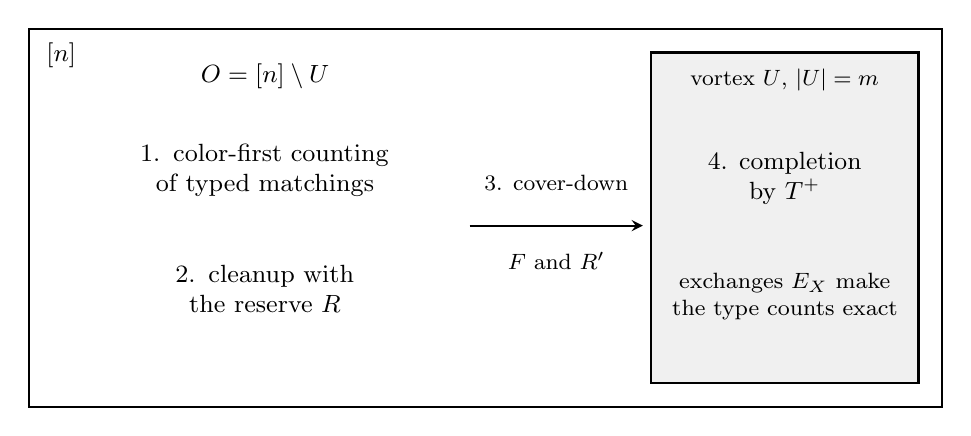
\begin{tikzpicture}[font=\small,>=stealth]
  \draw[thick] (0,0) rectangle (11.6,4.8);
  \node[anchor=north west] at (0.1,4.75) {$[n]$};
  \node at (3.0,4.2) {$O=[n]\setminus U$};
  \node[align=center,text width=4.2cm] at (3.0,3.0) {1. color-first counting of typed matchings};
  \node[align=center,text width=4.2cm] at (3.0,1.5) {2. cleanup with the reserve $R$};
  \draw[thick,fill=black!6] (7.9,0.3) rectangle (11.3,4.5);
  \node[font=\footnotesize] at (9.6,4.15) {vortex $U$, $|U|=m$};
  \node[align=center] at (9.6,2.9) {4. completion\\by $T^+$};
  \node[align=center,text width=3.0cm,font=\footnotesize] at (9.6,1.4) {exchanges $E_X$ make the type counts exact};
  \draw[->,thick] (5.6,2.3) -- (7.8,2.3);
  \node[font=\footnotesize,align=center] at (6.7,2.85) {3. cover-down};
  \node[font=\footnotesize,align=center] at (6.7,1.85) {$F$ and $R'$};
\end{tikzpicture}
\caption{Schematic of the lower-bound construction of Section 5 (not to scale). The vortex has $m\approx n^{1-\delta'/4}$ points.}
\end{figure}

Only stage 1 is counted. The other stages involve \(O(n^{2-\delta'/4})\) pairs, which costs \(O(n^{2-\delta'/4}\log n)\) in the logarithm. The vortex has polynomial size, but it tends to infinity, so Theorem T applies inside it with fixed constants.

\textbf{Constants.} The constants are chosen in the order below. Three of them, \(\gamma_S\), \(\lambda\) and \(c_\rho\), are minima of several terms, and we record where their terms are used.

\begin{enumerate}
\def\labelenumi{\arabic{enumi}.}
\item
  \textbf{\(C_0\), \(K_c\), \(C_1\), \(B\) and \(\gamma_S\).} Take \(K_c\) from Lemma 5.7, and \(C_0\) and \(C_1\) from Lemmas 5.8 and 5.10, for seeds with margin \(\zeta/4\) on \(U\); here \(C_1\) is the constant in \(\sigma\le C_1\Delta/m\) in the proof of Lemma 5.10. Take \(B\) from Lemma 5.8\('\). The vortex host \(G_U\) will satisfy \(\Delta(K[U]\setminus G_U)\le\gamma_S m\), and \(\gamma_S\) is the minimum of the following values, one for each use of that bound.

  \begin{itemize}
  \tightlist
  \item
    \(1/(4K_cC_0(C_1+2C_0))\), for Lemma 5.8. Since \(C_0\ge1\), it also gives \(4K_c\Delta\le m\).
  \item
    \(\zeta/(8B(K_cC_1+(K_c+1)C_0))\), for Lemma 5.8\('\).
  \item
    \(\delta_0/8\), for H3 and H4 through {[}10, Appendix B.4{]}. Every class of \(U\) has \(u_Y\ge\delta_0m-1\) points, so for large \(m\) two roots have at least \(u_Y-2(\Delta+1)\ge(\delta_0/2)m\) common neighbors in each class, and there are at least \((\delta_0m-4\Delta-6)^2\ge\delta_0^2m^2/5\) hinges on six vertices. This value also gives \(\delta(G_U)\ge(1-\gamma_S)m-1\ge7m/8-1\), as Section 5.8 uses.
  \item
    \(\delta_0/(2(k+4))\), for Lemma 5.9: any \(k+4\) points of \(U\) then have at least \(u_Y-(k+4)(\Delta+1)\ge(\delta_0/2)m-k-5>0\) common neighbors in every class \(U_Y\).
  \item
    \(d_0^5\delta_0\eta_1/20\), for Section 5.10, where \(\eta_1\) is the smaller of \(\eta_0\) of Lemma 5.19 and the bound on \(\eta'\) required in H1 there. Then \(\eta'\le10\gamma_S/(d_0^5\delta_0)+2\eta+m^{-1/3}\le\eta_1\) for large \(n\).
  \end{itemize}
\item
  \textbf{\(\theta_0\), \(\lambda\) and \(\eta_T\).} Put \(\theta_0:=(\delta_0/2)\min\{\delta_0,\zeta/2\}\), the share of each kind of block at a point in cover-down step 4 (Lemma 5.6). With \(J=\binom{k-1}{2}\), choose

  \[\lambda\le\min\Big\{\frac{\gamma_S}{36},\ \frac{\delta_0}{18(J+1)},\ \frac{\theta_0\delta_0}{200},\ \sqrt{\frac{\zeta}{40(J+B)}}\Big\},\]

  and put \(\eta_T=\lambda^2/256\). The four terms are used as follows.

  \begin{itemize}
  \tightlist
  \item
    \(\gamma_S/36\) gives \(\Delta(E_X)\le9\lambda m\le\gamma_S m/4\) in the bound on \(\Delta(D\cup E_X)\) below.
  \item
    \(\delta_0/(18(J+1))\) is the vertex budget of the exchange pools {[}10, §4.1{]}: each independent coordinate uses its own pools, so the union of the footprints has maximum degree at most \(9p_X\).
  \item
    \(\theta_0\delta_0/200\) bounds the exclusions caused by \(E_X\) in steps 4 and 5 of Lemma 5.6; it implies \(\lambda\le\theta_0/72\).
  \item
    \(\sqrt{\zeta/(40(J+B))}\) keeps the centered residual of Lemma 5.10 inside its margin: the high halves contain at most \(9Jp_X^2\) blocks of any one type, and the shift \(s_i/2\le p_X^2/2\) is extended with entries at most \(Bp_X^2/2\).
  \end{itemize}

  In Sections 5.8--5.10 and 6, \(J\) and \(B\) are those of the section.
\item
  \textbf{\(\alpha\), \(C\) and \(h\).} The bounds of Section 5.6 give H1, H3 and H4 of Theorem T with \(C=2C_0\), \(\alpha=\delta_0^2/5\) and \(h=6\).
\item
  \textbf{\(c_\rho\).} Choose

  \[c_\rho\le\min\{\gamma_S/12,\ \zeta/100,\ \theta_0/8\}.\]

  The term \(\gamma_S/12\) gives the bound on \(\Delta(D)\) below. The term \(\theta_0/8\) is used in steps 4 and 5 of Lemma 5.6, and \(\zeta/100\) in Section 5.7.

  Section 5.10 adds \(c_\rho\le d_0^3\theta_0/32\), \(\lambda\le\min\{d_0^3\theta_0/300,\,d_0^5\theta_0\delta_0/100\}\) and \(\lambda\le c(k,\delta_0,d_0)\), and Section 6.4 adds \(\lambda\le\delta_0/200\). These depend only on \(k\), \(d_0\), \(\delta_0\) and \(\theta_0\), which are fixed before \(\lambda\) and \(c_\rho\), so there is no circularity.
\item
  \textbf{\(\varepsilon_G\), \(\theta\) and \(\delta'\).} Take \(\varepsilon_G\in(0,\min\{\varepsilon_0,1/4\})\), where \(\varepsilon_0\) is given by {[}30, Theorem 3.5{]} for uniformity 3 and conflict parameter 2. Put \(\theta=\varepsilon_G^3/2\) and \(\delta'=\theta/20\).
\end{enumerate}

Table 3 summarizes this order.

\begin{longtable}[]{@{}
  >{\raggedright\arraybackslash}p{(\linewidth - 6\tabcolsep) * \real{0.0811}}
  >{\raggedright\arraybackslash}p{(\linewidth - 6\tabcolsep) * \real{0.2703}}
  >{\raggedright\arraybackslash}p{(\linewidth - 6\tabcolsep) * \real{0.2703}}
  >{\raggedright\arraybackslash}p{(\linewidth - 6\tabcolsep) * \real{0.3784}}@{}}
\caption{Order of choice of the constants of Section 5. Each row depends only on the hypotheses and the rows above it.}\tabularnewline
\toprule\noalign{}
\begin{minipage}[b]{\linewidth}\raggedright
Order
\end{minipage} & \begin{minipage}[b]{\linewidth}\raggedright
Constants
\end{minipage} & \begin{minipage}[b]{\linewidth}\raggedright
Chosen from
\end{minipage} & \begin{minipage}[b]{\linewidth}\raggedright
Used for
\end{minipage} \\
\midrule\noalign{}
\endfirsthead
\toprule\noalign{}
\begin{minipage}[b]{\linewidth}\raggedright
Order
\end{minipage} & \begin{minipage}[b]{\linewidth}\raggedright
Constants
\end{minipage} & \begin{minipage}[b]{\linewidth}\raggedright
Chosen from
\end{minipage} & \begin{minipage}[b]{\linewidth}\raggedright
Used for
\end{minipage} \\
\midrule\noalign{}
\endhead
\bottomrule\noalign{}
\endlastfoot
1 & \(C_0\), \(K_c\), \(C_1\), \(B\), \(\gamma_S\) & \(k\), \(\delta_0\), \(\zeta\) (and \(d_0\) in Section 5.10) & Seeds (Lemmas 5.8, 5.8\('\)), H3 and H4, Lemma 5.9, typical hosts \\
2 & \(\theta_0\), \(\lambda\), \(\eta_T\) & \(\delta_0\), \(\zeta\), \(\gamma_S\), \(J\), \(B\) (and \(k\), \(d_0\) in Section 5.10) & Exchange footprints and pools, exclusions in Lemma 5.6, centering in Lemma 5.10 \\
3 & \(\alpha\), \(C\), \(h\) & \(C_0\), \(\delta_0\) & H1, H3 and H4 of Theorem T \\
4 & \(c_\rho\) & \(\gamma_S\), \(\zeta\), \(\theta_0\) (and \(k\), \(d_0\) in Section 5.10) & Density of \(R'\): \(\Delta(D)\), steps 4 and 5 of Lemma 5.6, Section 5.7 \\
5 & \(\varepsilon_G\), \(\theta\), \(\delta'\) & {[}30, Theorem 3.5{]} (and \(c_0\) in Section 5.10) & Matching count, cleanup, size of the vortex \\
--- & \(\kappa\), \(u_X\), \(m\), \(\rho\), \(p\), \(d^*\), \(p_X\) & All of the above and \(n\) & Vortex and reserves \\
\end{longtable}

\textbf{Parameters depending on \(n\).} We put \(\kappa=n^{-\delta'/4}\); \(u_X=\lfloor\kappa c_X\rfloor\) for each class \(X\); \(m=\sum_Xu_X\); \(\rho=c_\rho\kappa\); \(p=n^{-\delta'}\); \(d^*=\lfloor m^{1/4}\rfloor\) made odd; and a prime \(p_X\in[\lambda m/4,\lambda m]\).

\textbf{The bound on \(\Delta(D\cup E_X)\).} Here \(D\) is the set of edges inside \(U\) of the cover-down packing (Lemma 5.6), and \(E_X\) is the graph of exchange footprints of Section 5.2. With the choices above, \(\Delta(D)\le3\rho n\le3c_\rho(m+k)\le(\gamma_S/4)(m+k)\), using \(\kappa n\le m+k\), and \(\Delta(E_X)\le9\lambda m\le\gamma_S m/4\). Consequently, \(\Delta(D\cup E_X)\le\gamma_S m/2+\gamma_S k/4\le\gamma_S m\) for \(m\ge k\). In Section 6 the same rules apply with \(J=(a-1)(b-1)(c-1)\), \(\Delta(D)\le3c_\rho(m+1)\) and \(\Delta(E_X)\le6\lambda m\).

\subsubsection{5.2 The vortex and the reserves}\label{the-vortex-and-the-reserves}

We now fix the vortex, the exchange footprints, the cover-down graph and two reserves; Lemma 5.1 lists the properties of these objects that the later stages use.

Fix \(U\) with \(|U\cap X|=u_X\) for every class \(X\), and put \(O=[n]\setminus U\) and \(o_X=c_X-u_X\). Call a pair \(\{x,x'\}\subset O\) \emph{compatible with} a class \(Y\) if the triple \(\{x,x',w\}\) is bicolored for \(w\in Y\). That is, either \(x,x'\) lie in one class \(X\ne Y\), or one of them lies in \(Y\) and the other in a class \(X\ne Y\).

We fix \(E_X\), \(F\) and \(R'\) independently, and then \(R\) given \(F\).

\begin{itemize}
\item
  \textbf{Exchange footprints \(E_X\subset K[U]\).} For each of the \(J\) independent coordinates of Sections 5.1 and 5.6, place \(p_X^2\) copies of the nine-point exchange of {[}10, §4.1{]} inside \(U\), with pairwise disjoint pair sets and separate point pools for different coordinates {[}10, §4.1{]}. Their union has maximum degree at most \(9p_X\le9\lambda m\).
\item
  \textbf{The cover-down graph \(F=\bigsqcup_YF_Y\subset K[O]\).} An edge between \(O\cap X\) and \(O\cap Y\) (\(X\ne Y\)) is placed in \(F_Y\) with probability

  \[q^Y_{XY}=\frac{2(1-\kappa)(1-\rho)\,u_Y\,t_{YX}}{c_Y\,o_X\,o_Y},\]

  and in \(F_X\) with probability \(q^X_{YX}\). An edge inside \(O\cap X\) is placed in \(F_Y\) (\(Y\ne X\)) with probability

  \[q^Y_{XX}=\frac{(1-\kappa)(1-\rho)\,u_Y\,t_{XY}}{c_Y\binom{o_X}{2}}.\]

  These events are disjoint for each edge, and all probabilities are \(O(\kappa)\). Every edge of \(F_Y\) is compatible with \(Y\).
\item
  \textbf{The cleanup reserve \(R\subset K[O]\setminus F\)}, binomial with density \(p\).
\item
  \textbf{The cover-down reserve \(R'\subset K[O,U]\)}, binomial with density \(\rho\).
\end{itemize}

For \(x\in O\cap X\) and every class \(Y\), the expected degree of \(x\) in \(F_Y\) is \((1-\rho)u_Y(1+O(1/(\kappa n)))\). Indeed, by (1.3), for \(X=Y\) the expectation is \((1-\kappa)(1-\rho)u_Y(c_Y-1)/o_Y\), and for \(X\ne Y\) it is \((1-\kappa)(1-\rho)u_Yc_X/o_X\). In both cases the ratio \((c-1)/o\) or \(c/o\) is \((1-\kappa)^{-1}(1+O(1/(\kappa n)))\). The blocks built on \(F_Y\) in Section 5.5 have the same type proportions as \(t\).

Every edge of \(K[O]\) lands, independently of the other edges, in exactly one of the graphs \(F_Y\) (\(Y\) a class), \(R\) and the \emph{availability graph} \(A=K[O]\setminus(F\cup R)\). An edge of class \(\pi\) lies in \(A\) with probability \(\nu_\pi\), defined in Section 5.3.

\Needspace{7\baselineskip}\textbf{Lemma 5.1.} With probability \(1-o(1)\) the following hold for all \(x\ne y\) in \(O\), all \(w\ne w'\) in \(U\) and all classes \(Y\).

\begin{itemize}
\tightlist
\item
  \textbf{F1.} \(\deg_{F_Y}(x)=(1-\rho)u_Y\pm\sqrt{\kappa n}\log n\).
\item
  \textbf{F2.} \(|N_{R'}(x)\cap U_Y|=\rho u_Y\pm\sqrt{\rho u_Y}\log n\), \(|N_{R'}(x)\cap N_{R'}(y)\cap U_Y|=\rho^2u_Y\pm\sqrt{\rho^2u_Y}\log n\), and \(|N_{R'}(w)\cap N_{R'}(w')|=\rho^2|O|\pm\sqrt{\rho^2n}\log n\).
\item
  \textbf{F3.} \(\deg_{R'}(w)=\rho|O|\pm\sqrt{\rho n}\log n\), and \(|N_{F_Y}(x)\cap N_{R'}(w)|=\rho\deg_{F_Y}(x)\pm\sqrt{\rho\kappa n}\log n\).
\item
  \textbf{F4.} \(|N_{R'}(x)\cap N_{E_X}(w)|\le9\rho\lambda m+\sqrt{\rho m}\log n\).
\item
  \textbf{F5.} \(e_F(S,T)\le|S||T|/4\) for disjoint \(S,T\subset O\) with \(|S|,|T|\ge s_2:=n^{1/2+\delta'}\).
\item
  \textbf{F6.} \(\deg_A(x,O\cap Z)=\nu_\pi|O\cap Z|\pm\sqrt n\log n\) for every class \(Z\), where \(\pi\) is the class pair of \(x\) and \(Z\).
\item
  \textbf{R1.} For at most three roots and one further vertex \(y\) of a prescribed class, the number of \(y\) whose edges to the roots lie in prescribed ones of the graphs \(F_Y\), \(R\) and \(A\) is within \(1\pm n^{-1/3}\) of its expectation, unless that expectation is 0.
\item
  \textbf{R2.} \(e_R(S,T)\ge p|S||T|/2\) for disjoint \(S,T\) with \(|S|,|T|\ge s_2\).
\item
  \textbf{R3.} For \(|T|\ge s_0/2\), where \(s_0:=20C_Ln^{1-\theta+2\delta'}\) with \(C_L\) the constant of Corollary 5.3, fewer than \(s':=2n^{2\delta'}\) vertices \(u\) have \(\deg_R(u,T)<p|T|/2\).
\end{itemize}

\emph{Proof.} F1--F4 follow from Chernoff bounds {[}31{]} and a union bound over \(n^{O(1)}\) events, since each count is a sum of independent indicators with mean of order at least \(n^{1-3\delta'/4}\). In F3 and F4 the graph \(R'\) is independent of \(F\) and of \(E_X\), which are fixed first. F4 is an upper-tail Chernoff bound. F6 is a Chernoff bound, since \(A\) has independent edges.

F5 is a Chernoff bound for each pair \((S,T)\): since \(F\) has edge probabilities \(O(\kappa)\), the event \(e_F(S,T)\ge|S||T|/4\) has probability \(\exp(-\Omega(|S||T|))\). The union bound over at most \(4^n\) pairs works because \(s_2^2=n^{1+2\delta'}\gg n\).

R1 is a Chernoff bound: for distinct \(y\) the indicators involve disjoint edges, and every nonzero expectation is at least \(c\cdot n\cdot\min(p,\kappa)^3\ge n^{1-4\delta'}\) for large \(n\). R2 follows from F5, since then \(\mathbb E\,e_R(S,T)\ge(3/4)p|S||T|\), together with a Chernoff bound and a union bound.

For R3, fix \(T\) with \(|T|=t\ge s_0\). Since \(R\) lives in \(K[O]\setminus F\), we first note that fewer than \(n^{2\delta'}\) vertices \(u\) have \(\deg_F(u,T)\ge t/4\). Indeed, for a set \(Z\) of \(n^{2\delta'}\) vertices, after discarding the at most \(n^{4\delta'}\) edges inside \(Z\), which \(Z\) and \(T\) may share, \(\mathbb P(e_F(Z,T)\ge|Z|t/4)\le2^{-|Z|t/5}\), and the union over \(\exp((t+|Z|)\log n)\) choices of \((Z,T)\) is \(o(1)\). For the other vertices, \(\mathbb E\deg_R(u,T)\ge(3/4)pt\). For a set \(Z\) of \(n^{2\delta'}\) such vertices, all of them have \(\deg_R(u,T)<pt/2\) with probability \(\exp(-\Omega(pt\,n^{2\delta'}))\), after discarding the at most \(n^{4\delta'}\) edges inside \(Z\). The union over the same choices is \(o(1)\), because \(p\,n^{2\delta'}=n^{\delta'}\gg\log n\). Consequently, fewer than \(2n^{2\delta'}=s'\) vertices \(u\) have \(\deg_R(u,T)<pt/2\).~\(\square\)

We fix such \(E_X\), \(F\), \(R\) and \(R'\).

\subsubsection{5.3 Color-first counting inside O}\label{color-first-counting-inside-o}

Stage 1 colors the available edges of \(K[O]\) at random by block type and, for each good coloring, counts the near-perfect matchings of the resulting typed 3-graphs. The color probabilities are fixed by a target type matrix \(t'\), and Lemma 5.2 shows that the count reproduces \(\Phi(t)\).

An edge of \(K[O]\) with labels \(\{X,X\}\) is \emph{available}, meaning it is not in \(F\cup R\), with probability

\nopagebreak[4]
\[\nu_{XX}=(1-p)\Big(1-\sum_{Y\ne X}q^Y_{XX}\Big).\]

An edge with labels \(\{X,Y\}\) is available with probability

\nopagebreak[4]
\[\nu_{XY}=(1-p)\big(1-q^X_{YX}-q^Y_{XY}\big).\]

All of these are \(1-O(\kappa+p)\).

The two families of equations in (5.1) below are consistent only if \(\sum_X\binom{o_X}{2}\nu_{XX}=\frac12\sum_{X<Y}o_Xo_Y\nu_{XY}\). For the classes themselves this is the admissibility identity, but after the rounding \(u_X=\lfloor\kappa c_X\rfloor\) the two sides differ by \(O(n)\). We therefore multiply every \(\nu_{XX}\) by the common factor \(\varphi=1+O(1/n)\) that makes them equal, and keep the notation \(\nu_{XX}\); the rescaled value stays below \(1\), since \(\nu_{XX}\le1-p\) and \(p\gg1/n\). Every estimate below that involves \(\nu_{XX}\) allows a relative error of order at least \(n^{-1/3}\), or an additive error \(O(n\log n)\) in the logarithm, so this factor is absorbed.

\textbf{The target of stage 1.} Fix a nonnegative matrix \(t'\) with

\nopagebreak[4]
\[\sum_{Y\ne X}t'_{XY}=\binom{o_X}{2}\nu_{XX},\qquad2(t'_{XY}+t'_{YX})=o_Xo_Y\nu_{XY},\tag{5.1}\]

and \(t'_{XY}=(1-\kappa)^2t_{XY}(1+O(\kappa))\). Its \(J\) free coordinates are fixed in Section 5.7. Put

\nopagebreak[4]
\[\beta_{XY}=\frac{t'_{XY}}{\binom{o_X}{2}\nu_{XX}},\qquad a_{XY}=\frac{2t'_{XY}}{o_Xo_Y\nu_{XY}}.\]

By (5.1), \(\sum_Y\beta_{XY}=1\) and \(a_{XY}+a_{YX}=1\). Let \(\mu\) be the product measure on colorings \(\chi\) of the available edges:

\begin{itemize}
\tightlist
\item
  an available edge inside \(X\) receives color \((X,Y)\) with probability \(\beta_{XY}\);
\item
  an available edge between \(X\) and \(Y\) receives \((X,Y)\) with probability \(a_{XY}\), and \((Y,X)\) otherwise.
\end{itemize}

For \(\tau=(X,Y)\), the 3-graph \(H_\tau(\chi)\) has as vertices the edges of color \(\tau\), and as edges the triangles \(\{x,x',y\}\), with \(x,x'\in X\) and \(y\in Y\), whose three edges have color \(\tau\). A matching in \(H_\tau(\chi)\) is thus a set of edge-disjoint blocks of type \(XXY\) inside \(O\).

\textbf{Degrees.} By R1 for the availability graph \(A\), in expectation over \(\chi\):

\begin{itemize}
\tightlist
\item
  an edge \(\{x,x'\}\) of color \(\tau\) lies in \(o_Y\nu_{XY}^2a_{XY}^2(1\pm n^{-1/3})\) triangles of \(H_\tau(\chi)\);
\item
  an edge \(\{x,y\}\) of color \(\tau\) lies in \((o_X-1)\nu_{XX}\nu_{XY}\beta_{XY}a_{XY}(1\pm n^{-1/3})\).
\end{itemize}

Since

\nopagebreak[4]
\[(o_X-1)\nu_{XX}\beta_{XY}=\frac{2t'_{XY}}{o_X}=o_Y\nu_{XY}a_{XY},\]

both equal \(D_\tau(1\pm n^{-1/3})\) with

\nopagebreak[4]
\[D_\tau=o_Y\nu_{XY}^2a_{XY}^2=\Theta(n).\]

Put \(\gamma'=2\delta'\). A coloring \(\chi\) is \emph{good} if it satisfies G1--G4 below. G1 and G2 give the hypotheses of the matching theorem, G3 controls the leftover at a vertex in the cleanup of Section 5.4, and G4 turns the measure of the set of good colorings into a lower bound on their number.

\begin{itemize}
\tightlist
\item
  \textbf{G1.} Every vertex of every \(H_\tau(\chi)\) has degree \(D_\tau(1\pm n^{-1/4})\).
\item
  \textbf{G2.} Color \(\tau\) is used on \(3t'_\tau\pm n^{1+\gamma'}\) edges.
\item
  \textbf{G3.} For every \(v\in O\cap X\) and \(Y\ne X\), the \emph{imbalance} \(\iota_Y(v)\) is at most \(n^{1/2+\gamma'}\) in absolute value. It is the number of available edges of color \((X,Y)\) inside \(X\) at \(v\), minus the number of available edges of color \((X,Y)\) from \(v\) to \(Y\). Their expectations agree, by the displayed identity above, up to the error in the available degrees, which is \(\sqrt n\log n\) by F6.
\item
  \textbf{G4.} \(|\log(1/\mu(\chi))-H(\mu)|\le n^{1+\gamma'}\).
\end{itemize}

Each condition fails with probability \(o(1)\), by Chernoff and Hoeffding bounds together with F6 and R1. For G4, write \(\log(1/\mu(\chi))=\sum_e\log(1/\mu_e(\chi(e)))\), a sum of at most \(n^2\) independent terms, one per available edge, with mean \(H(\mu)\). Every color probability is at least \(\zeta\) for large \(n\): \(t'_{XY}\ge(\zeta/2)n^2\), so \(\beta_{XY}=t'_{XY}/(\binom{o_X}{2}\nu_{XX})\ge2t'_{XY}/n^2\ge\zeta\), and likewise \(a_{XY}\ge\zeta\) and \(1-a_{XY}=a_{YX}\ge\zeta\). Hence each term lies in \([0,\log(1/\zeta)]\), and Hoeffding's inequality {[}32{]} gives

\nopagebreak[4]
\[\mu\big(|\log(1/\mu(\chi))-H(\mu)|>n^{1+\gamma'}\big)\le2\exp\big(-2n^{2\gamma'}/\log^2(1/\zeta)\big)=o(1).\]

Hence \(\mu(\mathrm{Good})\ge1/2\), where \(\mathrm{Good}\) is the set of good colorings. Every good \(\chi\) has \(\mu(\chi)\le e^{-H(\mu)+n^{1+\gamma'}}\), so \(1/2\le\mu(\mathrm{Good})\le|\mathrm{Good}|\,e^{-H(\mu)+n^{1+\gamma'}}\), that is,

\nopagebreak[4]
\[|\mathrm{Good}|\ge\tfrac12\exp\big(H(\mu)-n^{1+\gamma'}\big).\]

The lower bound uses only the half \(\log(1/\mu(\chi))\ge H(\mu)-n^{1+\gamma'}\) of G4; the other half comes from the same inequality. The same holds in Sections 5.8--5.10. There every color probability is a type count of at least \((\zeta/2)n^2\), times a bounded multiplicity, divided by a pair count of at most \(n^2\), times an availability factor \(1+O(\kappa+p)\). It follows that each probability is at least \(\zeta/4\) for large \(n\), and Hoeffding applies with \(\log(4/\zeta)\) in place of \(\log(1/\zeta)\).

The next lemma shows that the entropy of \(\mu\) and the logarithmic matching counts \(t'_\tau(\log D_\tau-2)\) add up to the rate \(\Phi(t)\).

\Needspace{7\baselineskip}\textbf{Lemma 5.2 (color-first identity).}

\nopagebreak[4]
\[H(\mu)+\sum_\tau t'_\tau(\log D_\tau-2)=\Phi(t)-O(n^{2-\delta'/4}\log n).\]

\emph{Proof.} By Chernoff bounds for the number of available edges of each class pair,

\nopagebreak[4]
\[H(\mu)=(1\pm n^{-1/3})\Big[\sum_X\binom{o_X}{2}\nu_{XX}H(\beta_{X\cdot})+\sum_{X<Y}o_Xo_Y\nu_{XY}H(a_{XY})\Big].\]

Since \(\binom{o_X}{2}\nu_{XX}\beta_{XY}=t'_{XY}\), the first sum is \(-\sum t'_{XY}\log\beta_{XY}\). Since \(o_Xo_Y\nu_{XY}a_{XY}=2t'_{XY}\), the second is \(-\sum2t'_{XY}\log a_{XY}\). Adding \(\sum t'_{XY}(\log(o_Y\nu_{XY}^2a_{XY}^2)-2)\), the terms in \(a\) cancel and \(o_Y\nu_{XY}^2/\beta_{XY}=N^O_{XY}\nu_{XX}\nu_{XY}^2/t'_{XY}\). This gives

\nopagebreak[4]
\[H(\mu)+\sum_\tau t'_\tau(\log D_\tau-2)=\sum_{X\ne Y}t'_{XY}\Big(\log\frac{N^O_{XY}}{t'_{XY}}-2\Big)+\sum_{X\ne Y}t'_{XY}\log(\nu_{XX}\nu_{XY}^2),\]

where \(N^O_{XY}=\binom{o_X}{2}o_Y\). The last sum is \(O((\kappa+p)n^2)\). Since \(N^O/t'=(1-\kappa)(N/t)(1+O(\kappa))\) and \(t'=(1-\kappa)^2t(1+O(\kappa))\), the first sum is \(\Phi(t)-O(\kappa n^2\log n)\). Finally \(\kappa n^2\log n=n^{2-\delta'/4}\log n\).~\(\square\)

\textbf{Matching counts.} Fix a good \(\chi\) and a color \(\tau\). We apply {[}30, Theorem 3.5{]} with \(k=3\), \(\ell=2\), an empty conflict system and \(d=d_\tau:=\Delta(H_\tau(\chi))\). Its hypotheses hold:

\begin{itemize}
\tightlist
\item
  \((1-d^{-\varepsilon_G})d\le\delta(H_\tau)\le\Delta(H_\tau)\le d\), by G1, since \(\varepsilon_G<1/4\);
\item
  \(\Delta_2(H_\tau)\le1\le d^{1-\varepsilon_G}\), since two edges lie in at most one common triangle;
\item
  \(|V(H_\tau)|\le n^2\le\exp(d^{\varepsilon_G^3})\);
\item
  the empty conflict system is trivially \((d,2,2,\varepsilon_G)\)-bounded.
\end{itemize}

The theorem gives a set \(\mathcal M_\tau(\chi)\) of at least \(((1-d^{-\varepsilon_G^4})d/e^2)^{m_\tau}\) matchings of size \(m_\tau=(1-d^{-\varepsilon_G^3})|V(H_\tau)|/3=t'_\tau(1\pm O(n^{-\varepsilon_G^3}))\), by G2. Hence

\nopagebreak[4]
\[\sum_\tau\log|\mathcal M_\tau(\chi)|\ge\sum_\tau t'_\tau(\log D_\tau-2)-O(n^{2-\varepsilon_G^4}\log n).\]

Together with the lower bound on \(|\mathrm{Good}|\) and Lemma 5.2, this gives the count of stage 1.

\Needspace{7\baselineskip}\textbf{Corollary 5.3.} \(\sum_{\chi\in\mathrm{Good}}\prod_\tau|\mathcal M_\tau(\chi)|\ge\exp(\Phi(t)-o(n^2))\). For each such \((\chi,M)\), the set \(L_0\) of available edges not covered by \(M\) has \(|L_0|\le C_Ln^{2-\varepsilon_G^3}\).

\emph{Proof.} The first bound follows from the bound on \(|\mathrm{Good}|\), the matching counts and Lemma 5.2. Each matching of \(\mathcal M_\tau(\chi)\) leaves \(d_\tau^{-\varepsilon_G^3}|V(H_\tau)|\) vertices of \(H_\tau\) uncovered, and \(d_\tau\ge D_\tau/2\ge\zeta^2\delta_0n/8\). Hence \(|L_0|\le C_Ln^{2-\varepsilon_G^3}\) with \(C_L=k^2(8/(\zeta^2\delta_0))^{\varepsilon_G^3}\).~\(\square\)

\subsubsection{5.4 Cleanup}\label{cleanup}

Stage 2 covers the leftover edges at the few vertices where the leftover \(L_0\) of stage 1 is dense, using blocks with one or two edges in the reserve \(R\). Afterward every vertex has small leftover degree; Lemma 5.4 states the bounds.

Fix a good \(\chi\) and \(M\in\prod_\tau\mathcal M_\tau(\chi)\), and let \(L_0\) be as in Corollary 5.3. All vertices below lie in \(O\), and step 3 chooses its point \(w\) in \(O\).

A vertex is \emph{bad} if its degree in \(L_0\) exceeds \(n^{1-\theta}\). Let \(\mathrm{Bad}\) be the set of bad vertices; then \(|\mathrm{Bad}|\le2|L_0|/n^{1-\theta}\le2C_Ln^{1-\theta}\).

For \(v\in\mathrm{Bad}\cap X\) and \(Y\ne X\), consider the following \(L_0\)-neighbors of \(v\) outside \(\mathrm{Bad}\):

\begin{itemize}
\tightlist
\item
  \(A_Y(v)\): the neighbors \(u\in X\) with \(vu\) of color \((X,Y)\);
\item
  \(B_Y(v)\): the neighbors \(w\in Y\) with \(vw\) of color \((X,Y)\);
\item
  \(C_Y(v)\): the neighbors \(w\in Y\) with \(vw\) of color \((Y,X)\).
\end{itemize}

Every triangle of \(M_{(X,Y)}\) through \(v\) uses one edge of color \((X,Y)\) inside \(X\) and one from \(v\) to \(Y\). Hence \(|A_Y(v)|-|B_Y(v)|\) differs from \(\iota_Y(v)\) by at most \(|\mathrm{Bad}|\). The leftover is locally balanced by color, independently of \(M\).

\textbf{Construction.} We process the vertices of \(\mathrm{Bad}\) in order, maintaining the set \(W\subseteq R\) of reserve edges already used. For \(v\):

\begin{enumerate}
\def\labelenumi{\arabic{enumi}.}
\tightlist
\item
  Find a matching in \((R\setminus W)[A_Y(v),B_Y(v)]\). Each matched pair \(u,w\) gives the block \(\{v,u,w\}\) of type \(XXY\).
\item
  Find a matching in \((R\setminus W)[C_Y(v)]\). Each matched pair \(w,w'\) gives the block \(\{v,w,w'\}\) of type \(YYX\).
\item
  Cover every remaining \(L_0\)-edge \(vu\), including edges to other bad vertices, by a block \(\{v,u,w\}\) with \(vw,uw\in R\setminus W\). Choose \(w\notin\mathrm{Bad}\) uniformly among the common neighbors of compatible class; by R1 there are at least \(p^2\delta_0n/4\) of them.
\item
  Lists of size less than \(s_0\) go directly to step 3.
\end{enumerate}

A block of step 1 or step 2 covers two \(L_0\)-edges at \(v\) and uses one reserve edge away from \(v\); a block of step 3 covers one \(L_0\)-edge at \(v\) and uses two reserve edges, one of them at \(v\). Claim A bounds what steps 1 and 2 leave for step 3, and Claim B bounds the reserve edges that step 3 uses at \(v\).

\Needspace{7\baselineskip}\textbf{Claim A.} If \(|A_Y(v)|,|B_Y(v)|\ge s_0\), step 1 leaves at most \(|\iota_Y(v)|+|\mathrm{Bad}|+s_2+s'\) points of each list unmatched. If \(|C_Y(v)|\ge2s_0\), step 2 leaves at most \(n^{1/2+\gamma'}+s_2+s'\) points of each half unmatched, since the random halves differ in size by \(O(\sqrt n\log n)\), so each has at least \((1-o(1))s_0\) points. Shorter lists go directly to step 3.

\emph{Proof for step 1, by Hall's theorem.} Let \(A'\) be \(A_Y(v)\) minus the fewer than \(s'\) vertices badly connected to \(B_Y(v)\), as given by R3.

We first bound the degree of \(W\) away from the bad vertices: at all times, \(\Delta_W(u)\le(2C_L+o(1))n^{1-\theta}\) for every \(u\notin\mathrm{Bad}\). Indeed, each bad vertex \(v\) uses at most one reserve edge at \(u\) directly, for the \(L_0\)-edge \(vu\) (in step 1, 2 or 3), and with high probability the load from step 3 at any \(w\) is \(O(n^{1-\theta-\delta'}+\log^2n)\). For the load, step 3 makes at most \(2|L_0|\le2C_Ln^{2-2\theta}\) choices, each picking a given \(w\) with probability at most \(4/(p^2\delta_0n)\), so Freedman's inequality {[}33{]} gives load at most \(16C_Ln^{1-2\theta+2\delta'}/\delta_0+\log^2n\), and \(\theta=20\delta'>3\delta'\).

We now check Hall's condition for a set \(S\subseteq A'\).

\begin{itemize}
\tightlist
\item
  If \(|S|\le\sigma:=5C_Ln^{1-\theta+\delta'}\), every \(u\in S\) has degree into \(B_Y(v)\) in \(R\setminus W\) at least \(p|B_Y(v)|/2-\Delta_W\ge ps_0/2-(2C_L+o(1))n^{1-\theta}\ge\sigma\ge|S|\), since \(|B_Y(v)|\ge s_0\). For \(|S|>\sigma\) below, \(p|S|/2>(5C_L/2)n^{1-\theta}>\Delta_W\).
\item
  If \(|S|>\sigma\), let \(T=B_Y(v)\setminus N(S)\). If \(|T|\ge s_2\), then R2 gives \(e_R(S,T)\ge p|S||T|/2>|T|\Delta_W\ge e_W(S,T)\), contradicting \(e_{R\setminus W}(S,T)=0\). Therefore \(|T|<s_2\).
\end{itemize}

Hence the Hall deficiency of \(A'\) is at most \(\max\{0,|A'|-|B_Y(v)|\}+s_2\), so at most \((|A_Y(v)|-|B_Y(v)|)^++s_2+s'\) points of \(A_Y(v)\) and at most \((|B_Y(v)|-|A_Y(v)|)^++s_2+s'\) points of \(B_Y(v)\) remain unmatched. Step 2 reduces to step 1 by splitting \(C_Y(v)\) at random into two halves; lists \(C_Y(v)\) with fewer than \(2s_0\) points go directly to step 3.~\(\square\)

\Needspace{7\baselineskip}\textbf{Claim B.} Each bad vertex \(v\) has at most \(3(k-1)(2s_0+n^{1/2+\gamma'}+|\mathrm{Bad}|+s_2+s')+2|\mathrm{Bad}|\le C'n^{1-\theta+2\delta'}\) edges of \(W\) at itself: one for each \(L_0\)-edge covered by its own step 3, and at most one for each other bad vertex. This is much less than \(p^2n\). Its own steps 1 and 2 use no reserve edges at \(v\).

The outcome is a packing \(P_c\) of blocks of the allowed types with \(|P_c|\le C_Ln^{2-\theta}\). After removing it:

\begin{itemize}
\tightlist
\item
  every vertex has \(L_0\)-degree at most \(n^{1-\theta}\);
\item
  \(W\) has degree at most \((2C_L+o(1))n^{1-\theta}\) outside \(\mathrm{Bad}\) and at most \(C'n^{1-\theta+2\delta'}\) on \(\mathrm{Bad}\).
\end{itemize}

The edges of \(K[O]\setminus F\) that remain after stages 1 and 2 form the set \(L\) that the cover-down of Section 5.5 receives.

\Needspace{7\baselineskip}\textbf{Lemma 5.4.} Let \(L\) be the set of edges of \(K[O]\setminus F\) not covered by \(M\cup P_c\). Then

\nopagebreak[4]
\[\Delta(L)\le2n^{1-\delta'},\qquad|L|\le n^{2-\delta'}.\]

The graphs \(F\) and \(R'\) are untouched.

\emph{Proof.} \(L\) consists of \(R\setminus W\) and of the \(L_0\)-edges not covered by \(P_c\). The first has maximum degree \((1+o(1))pn\) by R1, and the second at most \(n^{1-\theta}\). Since \(\delta'<\theta\), this gives the degree bound. Also \(|L|\le|O|\,\Delta(L)/2\le n^{2-\delta'}\).~\(\square\)

\subsubsection{5.5 Cover-down}\label{cover-down}

The cover-down covers every pair with an endpoint in \(O\) that the earlier stages left uncovered, using bicolored blocks with one or two points in \(U\). For \(x\in O\cap X\), a block \(\{x,w,w'\}\) with \(w,w'\in U\) is bicolored exactly when the classes of \(w\) and \(w'\) are \(\{X,Y\}\) or \(\{Y,Y\}\) for some \(Y\ne X\). The next lemma bounds the size of every class; step 3 of the proof of Lemma 5.6 uses it to show that the points of \(U\) left at \(x\) do not lie mostly in the class of \(x\).

\Needspace{7\baselineskip}\textbf{Lemma 5.5 (bounded classes).} For every class \(X\), \(c_X\le(n+1)/2-\zeta n\).

\emph{Proof.} At a point of \(X\) there are \(c_X-1=\sum_Y2t_{XY}/c_X\) pairs inside \(X\), and \(n-c_X=\sum_{Y\ne X}2(t_{XY}+t_{YX})/c_X\ge c_X-1+2\zeta n\) pairs to other classes, since \(t_{YX}\ge\zeta n^2\) and \(c_X\le n\). Hence \(2c_X\le n+1-2\zeta n\).~\(\square\)

\Needspace{7\baselineskip}\textbf{Lemma 5.6 (cover-down).} There is a packing \(P\) of bicolored blocks, each with one or two points in \(U\), which covers every edge of \(F\cup L\cup K[O,U]\) exactly once and no other edge with a point in \(O\). The set \(D\) of its edges inside \(U\) is disjoint from \(E_X\) and satisfies \(\Delta(D)\le3\rho n\). The type counts of its blocks of step 1 are determined up to an error \(m^{2-1/1000}\); the blocks of step 2 are counted in Section 5.7. It has at most \(\rho nm(1+o(1))\) blocks with two points in \(U\).

\emph{Proof.} We build \(P\) in five steps. Step 1 covers almost all of \(F\) by blocks with one point in \(U\), and step 2 covers the remaining pairs inside \(O\) greedily, through the reserve \(R'\). After these two steps every pair inside \(O\) is covered, and the uncovered pairs at a point \(x\in O\) join \(x\) to a set \(S_x\subset U\). Step 3 records the properties of \(S_x\) that the later steps use. Step 4 covers almost all pairs \(xw\) with \(w\in S_x\) by blocks with two points in \(U\), and step 5 covers the few pairs that remain by switching blocks of step 4.

Steps 1 and 4 rely on the pseudorandom matching theorem of Ehard, Glock and Joos {[}19, Theorem 1.2{]}, formalized in {[}20{]}. For a 3-graph \(H\) with maximum degree at most \(\Delta\), codegrees at most \(\Delta^{1/2}\), and \(|H|\le\exp(\Delta^{1/810000})\), it gives a matching \(M\subseteq H\) such that every one of at most \(\exp(\Delta^{1/810000})\) prescribed nonnegative weight functions \(w\) with \(\max w\cdot\Delta^{3/2}\le w(H)\) satisfies

\nopagebreak[4]
\[w(M)=(1\pm\Delta^{-1/900})\,w(H)/\Delta.\]

We use it twice, with codegrees at most 1 and polynomially many weights. Every weight function below is the indicator of a set of edges of \(H\), so the matching contains a proportion \((1\pm\Delta^{-1/900})/\Delta\) of each prescribed set.

\emph{Step 1: blocks with one point in \(U\).} This step covers almost all edges of \(F\), together with edges between \(O\) and \(U\) outside \(R'\). For each class \(Y\) let \(H_Y\) be the 3-graph whose vertices are the edges of \(F_Y\) and the edges \(xw\) with \(x\in O\), \(w\in U_Y\) and \(xw\notin R'\). Its edges are the triples \(\{xx',xw,x'w\}\) with \(xx'\in F_Y\), \(w\in U_Y\) and \(xw,x'w\notin R'\). Each of them is a bicolored block, because \(F_Y\) is compatible with \(Y\). By F1--F3, every vertex has degree \((1-\rho)^2u_Y\pm O(\sqrt{\kappa n}\log n)\). We take \(\Delta\) to be the maximum degree, and use the weight functions given by the edges through a vertex \(x\in O\), the edges through a vertex \(w\in U_Y\), and the edges of each label type. The resulting matching \(M_Y\) leaves, at every \(x\in O\), at most \(m^{1-1/1000}\) uncovered edges of \(F_Y\) and at most \(m^{1-1/1000}\) uncovered edges \(xw\notin R'\), and, at every \(w\in U_Y\), at most \(nm^{-1/1000}=o(\rho^2n)\) uncovered edges \(xw\notin R'\). Let \(L_1\) be the set of uncovered edges of \(F\). This step uses no edge of \(R'\). The label-type weights have \(w(H_Y)/\Delta=O(nm)\), so the type counts of the blocks of step 1 are determined up to \(O(nm^{1-1/900})\le m^{2-1/1000}\), because \(m=(1+o(1))n^{1-\delta'/4}\) and \(\delta'=\varepsilon_G^3/40<4/9001\).

\emph{Step 2: remaining pairs inside \(O\).} This step covers the edges of \(L\cup L_1\), which have small maximum degree, by blocks whose two edges to \(U\) lie in \(R'\). Every edge \(xx'\in L\cup L_1\) is covered greedily by a block \(\{x,x',w\}\) with \(xw,x'w\in R'\) unused and \(w\) in a class compatible with \(xx'\). By F2 and Lemma 5.4 there are at least \(\rho^2u_Y/4\) candidates, since \(\rho^2u_Y\gg\Delta(L\cup L_1)\), and we choose \(w\) uniformly among them. By Freedman's inequality {[}33{]} (formalized in {[}20{]}), every \(w\in U\) then loses \(o(\rho n)\) edges of \(R'\). The load is \(O(n^{1-\delta'}/\kappa^2)\), which is \(o(\rho n)\) but of the order of \(\rho^2n\); the later steps only need \(o(\rho n)\). Every \(x\in O\) loses at most \(3n^{1-\delta'}\).

\emph{Step 3: the sets \(S_x\).} For \(x\in O\) let \(S_x\subset U\) be the set of \(w\) with \(xw\) still uncovered. By F2 and the bounds of steps 1 and 2, \(|S_x\cap U_Y|=\rho u_Y(1\pm o(1))\) for every \(Y\), and \(|S_x\cap S_{x'}|=\rho^2m(1\pm o(1))\) for all \(x\ne x'\). Moreover \(|S_x|\) is even, because every degree in \(K_n\) minus a packing is even and all edges of \(x\) inside \(O\) are covered. By Lemma 5.5, \(|S_x\cap X|\le(1/2-\zeta/2)|S_x|\) for \(x\in X\). Hence \(S_x\) has a perfect matching into allowed pairs. Step 4 uses the sizes of the sets \(S_x\cap U_Y\) and the bound on \(|S_x\cap X|\) to group the points of \(S_x\); steps 4 and 5 use the intersections, and step 5 uses the parity.

\emph{Step 4: blocks with two points in \(U\).} This step covers almost all pairs \(xw\) with \(w\in S_x\), again with the theorem of {[}19{]}. Its matching must also leave at every point \(x\) many blocks of each kind, and spread out its edges inside \(U\), because step 5 switches these blocks. For \(x\in X\), partition \(S_x\) at random into \emph{bipartite groups}, each formed by a set of \(d^*\) points of \(X\cap U\) and a set of \(d^*\) points of \(Y\cap U\) for some \(Y\ne X\), and \emph{internal groups}, each formed by \(d^*+1\) points of one class \(Y\ne X\).

The numbers of groups are fixed as follows. Write \(s=|S_x|\) and \(S_x^Y=S_x\cap U_Y\). For each \(Y\ne X\) put \(a_Y=|S_x^X|\cdot|S_x^Y|/\sum_{Y'\ne X}|S_x^{Y'}|\). There are \(\lfloor a_Y/d^*\rfloor\) bipartite groups with classes \(X\) and \(Y\), and the remaining points of \(S_x^Y\) form \(\lfloor(|S_x^Y|-d^*\lfloor a_Y/d^*\rfloor)/(d^*+1)\rfloor\) internal groups. Since \(|S_x^X|\le(1/2-\zeta/2)s\), we have \(a_Y\le|S_x^Y|\), so this is possible, and at most \(2k(d^*+1)\) points of \(S_x\) remain ungrouped. Since the partition is uniformly random, a Chernoff bound over the independent partitions shows that every \(w\in U\) is ungrouped at \(O(d^*\rho n/s)=O(d^*/\kappa)=o(s)\) points \(x\). By step 3, \(|S_x^Y|\ge\delta_0s(1-o(1))\) for every class \(Y\). Hence \(a_Y\ge\delta_0^2s(1-o(1))\). The points of \(S_x^Y\) left for internal groups number at least \(|S_x^Y|-a_Y\ge\zeta|S_x^Y|\ge\zeta\delta_0s(1-o(1))\), because \(\sum_{Y'\ne X}|S_x^{Y'}|-|S_x^X|=s-2|S_x^X|\ge\zeta s\). These two lower bounds supply the blocks of each kind counted at the end of this step.

Let \(H'\) be the 3-graph whose vertices are the edges \(xw\) with \(w\) grouped at \(x\), and the edges of \(K[U]\setminus E_X\). Its edges are the triples \(\{xw,xw',ww'\}\) with \(w,w'\) in one group of \(x\), on opposite sides if the group is bipartite. Since the vertices inside \(U\) avoid \(E_X\), so do the blocks of this step; the cost is a small loss in the degrees. Every vertex \(xw\) has degree \(d^*-e_x(w)\), where \(e_x(w)\) is the number of partners \(w'\) of \(w\) in its group with \(ww'\in E_X\). By F4 and a Chernoff bound over the grouping, \(e_x(w)\le10\lambda d^*/\delta_0\) for all \(x\) and \(w\), since the partners of \(w\) form a uniform subset of \(S_x\cap U_B\) of size at most \(d^*+1\), where \(U_B\) is the class of the partners, and \(|S_x\cap U_B|\ge\rho\delta_0m(1-o(1))\). By Chernoff over the independent groupings, every vertex \(ww'\) has degree at most \((c_\rho/\delta_0+o(1))d^*\le d^*/2\): a fixed \(w'\) lies in the group of \(w\) at \(x\) with probability at most \((d^*+1)/|S_x\cap U_B|\approx d^*/(\rho u_B)\), and \(|\{x:w,w'\in S_x\}|\le\rho^2|O|(1+o(1))\). Here \(c_\rho\le\theta_0/8\le\delta_0/2\).

We apply {[}19{]} with \(\Delta=d^*\) and the following four families of weight functions:

\begin{enumerate}
\def\labelenumi{\arabic{enumi}.}
\tightlist
\item
  for each \(x\), the edges at \(x\);
\item
  for each pair \((x,w)\), the edges \(\{x'w,x'z,wz\}\) with \(x'\ne x\) and \(z\in S_x\);
\item
  for each \(w\in U\), the edges containing a vertex of the form \(x'w\);
\item
  for each pair \(x\ne x'\), the edges at \(x'\) with a point in \(S_x\).
\end{enumerate}

The first family bounds the uncovered points at \(x\), the third and fourth bound the uncovered points at other points \(x'\), and the second controls the edges of the matching inside \(U\). Let \(M'\) be the resulting matching.

Since the degrees of \(H'\) fall short of \(d^*\) by \(e_x(w)\), the first family shows that \(M'\) leaves at most

\nopagebreak[4]
\[\sum_w e_x(w)/d^*+(d^*)^{-1/900}|S_x|+2k(d^*+1)\le(10\lambda/\delta_0+o(1))s\]

points of \(S_x\) uncovered. In the same way, by the third family, for each \(w\) the points \(x'\) at which \(w\) is uncovered number at most \((10\lambda/\delta_0+o(1))\rho n\), and by the fourth family at most \((10\lambda/\delta_0+o(1))|S_x\cap S_{x'}|\) uncovered points of \(x'\) lie in \(S_x\). Since \(10\lambda/\delta_0\le\theta_0/20\), for every class \(Y\ne X\), at least \(\theta_0s\) blocks \(\{x,z,z'\}\) of \(M'\) have \(z\in X\) and \(z'\in Y\), and at least \(\theta_0s\) have \(z,z'\in Y\), where \(\theta_0=(\delta_0/2)\min\{\delta_0,\zeta/2\}\) is the constant of Section 5.1.

By Hoeffding's inequality, the second family has total weight \((1+o(1))\rho^2nd^*\). The set \(D_1\) of edges of \(M'\) inside \(U\) satisfies

\nopagebreak[4]
\[|N_{D_1}(w)\cap S_x|\le(1+o(1))c_\rho|S_x|\qquad\text{for all }x\text{ and }w.\]

We call this the dispersion bound; step 5 uses it.

\emph{Step 5: repair.} This step covers the points of each \(S_x\) left uncovered by \(M'\). Pair up the uncovered points of \(S_x\), which are even in number. For a pair \(w,w'\), choose a block \(\{x,z,z'\}\) of \(M'\) at \(x\), not used by an earlier repair, such that \(\{x,w,z\}\) and \(\{x,w',z'\}\) are bicolored and \(wz,w'z'\notin D\cup E_X\), uniformly among such blocks. Replace \(\{x,z,z'\}\) by \(\{x,w,z\}\) and \(\{x,w',z'\}\); the pair \(zz'\) returns to the leftover inside \(U\). We show first that at least \(\theta_0s\) blocks at \(x\) are eligible for the pair \(w,w'\), that is, give two bicolored blocks, and then that at least \((3\theta_0/8)s\) of them survive the exclusions, so that the choice is always possible.

\emph{Eligible blocks.} Let \(w\in U_A\) and \(w'\in U_{A'}\), with \(x\in X\). A block with \(z\in X\) and \(z'\in Y\) can serve with \(z\) matched to \(w\) if \(A\ne X\) and \(A'\in\{X,Y\}\), and with \(z\) matched to \(w'\) if \(A'\ne X\) and \(A\in\{X,Y\}\). A block with \(z,z'\in Y\) can serve if \(A,A'\in\{X,Y\}\). Therefore:

\begin{itemize}
\tightlist
\item
  if \(A=A'=X\), every internal block serves;
\item
  if \(A=X\) and \(A'=B\ne X\) (or the reverse), the internal blocks of class \(B\) and the bipartite blocks of classes \(X,B\) serve;
\item
  if \(A,A'\ne X\), the bipartite blocks of classes \(X,A\) serve.
\end{itemize}

In every case at least \(\theta_0s\) blocks are eligible before exclusions, by step 4.

\emph{Exclusions.} A block is excluded if \(wz\) or \(w'z'\) lies in \(D\cup E_X\), or if it was used by an earlier repair at \(x\). We bound the exclusions caused by \(D_1\), by \(E_X\), by earlier repairs at \(x\), and by edges that repairs at other points add to \(D\).

By the dispersion bound of step 4, \(D_1\) excludes at most \(2(1+o(1))c_\rho s\le(1/4+o(1))\theta_0s\) blocks, since \(c_\rho\le\theta_0/8\). Since \(S_x\subset N_{R'}(x)\) up to \(O(m^{1-1/1000})\) points, F4 bounds the exclusions by \(E_X\) by \(2(9\rho\lambda m+o(s))\le(1/4+o(1))\theta_0s\), since \(s=\rho m(1+o(1))\) and \(\lambda\le\theta_0/72\). Earlier repairs at \(x\) number at most \((5\lambda/\delta_0+o(1))s\).

Repairs at other points \(x'\) add edges \(wz\) with \(z\in S_x\) in two ways. We bound both under the assumption that at least \((3\theta_0/8)s\) eligible blocks remain at every point; the resulting bounds maintain this assumption. First, \(w\) may be uncovered at \(x'\). By the third weight family this happens for at most \((10\lambda/\delta_0+o(1))\rho n+O(d^*/\kappa)\) points \(x'\). Then \(z\) is a point of a uniform eligible block, and lies in \(S_x\) with probability at most \(|S_x\cap S_{x'}|/((3\theta_0/8)s)\approx8\rho/(3\theta_0)\). This gives at most \((8\rho/(3\theta_0))(10\lambda/\delta_0)\rho n+o(s)\le(10\lambda/(3\delta_0)+o(1))s\) edges at \(w\), since \(\rho^2n\le c_\rho s(1+o(1))\) and \(c_\rho\le\theta_0/8\). Second, \(w\) may lie in the block chosen at \(x'\). This concerns only the \(x'\) with \(w\in S_{x'}\) and, for each uncovered point of \(x'\) in \(S_x\), happens with probability at most \(8/(3\theta_0s)\), so the fourth family gives the same bound. The same two bounds hold at \(w'\), and a block is excluded by an edge at either point. Freedman's inequality makes these bounds hold for all \((w,x)\).

Hence at least \((\theta_0/2-(55/3)\lambda/\delta_0-o(1))s\ge(3\theta_0/8)s\) blocks remain, because \(\lambda\le\theta_0\delta_0/200\), and the repair succeeds.

Each repair adds two edges to \(D\) and removes one. Thus \(\Delta(D)\le2\rho n+o(\rho n)\le3\rho n\).~\(\square\)

\subsubsection{5.6 Completion inside U}\label{completion-inside-u}

After the cover-down, every uncovered pair lies inside \(U\). We decompose these pairs into bicolored triangles with the absorption theorem \(T^+\), so that together with the blocks already placed there are exactly \(t_{XY}\) blocks of each type \(XXY\). Let \(P_{\mathrm{all}}=M\cup P_c\cup P\) be the packing built so far, and let \(G_U=K_n\setminus\bigcup P_{\mathrm{all}}\) minus the footprints \(E_X\). Every edge of \(G_U\) lies inside \(U\), and \(\Delta(K[U]\setminus G_U)\le\Delta(D\cup E_X)\le\gamma_Sm\) by the choice of \(c_\rho\) and \(\lambda\). For the absorption theorem \(T\) we label each point by its class and allow the bicolored types. Appendix A states \(T\) and \(T^+\).

Lemma 5.10 checks the hypotheses of \(T^+\) on \(G_U\). Lemmas 5.7 and 5.8 give an exact seed on a host that differs from \(K[U]\) by a graph of small maximum degree, Lemma 5.8\('\) makes the type masses of the seed exact, and Lemma 5.9 gives the lattice condition.

\textbf{Lemma 5.7 (bounded right inverse, {[}10, Lemma B.1{]}).} Let \(\ell(r)\) be the sum of \(r\) over cross edges minus twice its sum over internal edges. Let \(k\ge3\) and let \(A\) be the incidence map between the edges and the bicolored triangles of \(K[U]\). Then \(A\) has a linear right inverse \(\Psi\) on \(\{\ell=0\}\) with \(\|\Psi r\|_\infty\le K_c\|r\|_\infty/m\), where \(K_c=\binom{k-1}{2}\cdot400R^6(1+4R^2)\) and \(R=2/\delta_0\).

\emph{Proof.} {[}10, Lemma B.1{]} needs every class to have at least \(c^*\ge4\) points and the order to be at most \(Rc^*\). Here every class of \(U\) has \(u_Y\ge\delta_0m-1\ge\delta_0m/2\) points for large \(m\), so \(c^*=\delta_0m/2\) and \(R=2/\delta_0\) work.~\(\square\)

\Needspace{7\baselineskip}\textbf{Lemma 5.8 (exact seed).} Let \(D'\subset K[U]\) have maximum degree \(\Delta\) and put \(G'=K[U]\setminus D'\), with \(\ell(\mathbf 1_{E(G')})=0\). Let \(\mu_0\) be a weighting of the bicolored triangles of \(K[U]\) with \(1/(C_0m)\le\mu_0\le C_0/m\) and \(\|A\mu_0-1\|_\infty\le\sigma\). Suppose

\nopagebreak[4]
\[4K_c\Delta\le m\qquad\text{and}\qquad4K_cC_0(\sigma+2C_0\Delta/m)\le1.\]

Then \(G'\) has an exact seed \(\mu\), with \(A\mu=1\) on \(E(G')\) and \(1/(2C_0m)\le\mu\le2C_0/m\) on its bicolored triangles. Moreover, every test \(w\) with \(0\le w\le1\) satisfies \(|\sum\mu w-\sum\mu_0w|\le K_c\sigma m^2+(K_c+1)C_0\Delta m\).

\emph{Proof.} Call a triangle bad if it contains an edge of \(D'\), and good otherwise; let \(g\) and \(b\) be the restrictions to good and bad triangles. Put \(r_0=\mathbf 1_{E(G')}-Ag\mu_0\). This vector vanishes on \(D'\) and has \(\ell(r_0)=0\). Moreover \(\|r_0\|\le\sigma+2C_0\Delta/m\), since a surviving edge lies in at most \(2\Delta\) bad triangles.

The operator \(R_0=Ab\Psi\) preserves the space of vectors with \(\ell=0\) that vanish on \(D'\), and has norm at most \(2\Delta K_c/m\le1/2\) there. \(R_0\) preserves vanishing on \(D'\) because \(A\Psi x=x\) and good triangles avoid \(D'\). Let \(x=\sum_{s\ge0}R_0^sr_0\) and \(\psi=\Psi x\). Then \(Ag\psi=r_0\) and \(\|\psi\|\le2K_c\|r_0\|/m\le1/(2C_0m)\). Consequently, \(\mu=g(\mu_0+\psi)\) works. The mass bound counts the at most \(m^3/6\) changed weights and the at most \(\Delta m^2/2\) removed triangles.~\(\square\)

This is {[}10, Lemma B.2{]} with two changes: \(\mu_0\) need only be approximately exact, and \(D'\) need not be a union of triangles.

Lemma 5.8 moves the type masses by up to \(K_c\sigma m^2+(K_c+1)C_0\Delta m\), a constant fraction of \(m^2\) since \(\Delta\) is a constant fraction of \(m\). The exchange reserve only absorbs errors of order \(\lambda^2m^2\), with \(\lambda\le\gamma_S/36\). Thus the masses of the seed must be made exact before \(T^+\) is applied. This is the cube argument of {[}10, §3.3{]}, which we state in the generality needed here.

A \emph{pair-preserving change} is a change of the type vector that leaves every pair identity unchanged. Fix \(J\) independent coordinates \(I\) and pair-preserving changes \(b_1,\dots,b_J\) with \((b_j)_i=[i=j]\) for \(i\in I\), and put \(B=\max_\varepsilon\|\sum_j\varepsilon_jb_j\|_\infty\) over \(\varepsilon\in\{\pm1\}^J\). For bicolored types, the circulations on the triangles \(oXY\) of \(K_k\) (\(X,Y\ne o\)) give \(B\le k\). For Latin outlines, the alternating tensors of Lemma 6.6 with corner \((1,1,1)\) give \(B\le(a-1)(b-1)(c-1)\). In general the pair identities determine the dependent coordinates linearly from the free ones, so \(b_j\) can be taken as the real pair-preserving change with free coordinates \(e_j\); its entries are bounded in terms of \(k\) and \(\ell\). In Section 5.9 integer vectors are available: with free coordinates \(d(\pi,\Gamma)\) for class pairs \(\pi\not\ni o\) and color classes \(\Gamma\ne\omega\), the simple swaps of Lemma 5.18 have unit coordinates (see after its proof), so \(B\) depends only on \(k\) and \(\ell\).

\Needspace{7\baselineskip}\textbf{Lemma 5.8\('\) (exact masses).} Let \(G'\) be a graph on \(U\) and \(r\) a type vector that satisfies the pair identities of \(G'\). Let \(0\le E<\rho_c\). Suppose that for every corner \(r^\varepsilon=r+\rho_c\sum_j\varepsilon_jb_j\) (\(\varepsilon\in\{\pm1\}^J\)) there is an exact seed \(\mu^\varepsilon\) on \(G'\) with \(1/(Cm)\le\mu^\varepsilon\le C/m\) on its allowed triangles and \(|M_i(\mu^\varepsilon)-r^\varepsilon_i|\le E\) for every \(i\in I\), where \(M_i(\mu)\) is the mass of type \(i\). Then some convex combination \(\mu\) of the \(\mu^\varepsilon\) is an exact seed on \(G'\) with the same bounds and with \(M(\mu)=r\).

\emph{Proof.} Let \(P\) be the convex hull of the vectors \((M_i(\mu^\varepsilon))_{i\in I}\). Suppose that \((r_i)_{i\in I}\notin P\). Then a nonzero functional \(f\) separates it: \(f\cdot r>f\cdot M(\mu^\varepsilon)\) for every \(\varepsilon\). Take \(\varepsilon_j=\operatorname{sign}f_j\), with either sign when \(f_j=0\). Then \(f\cdot M(\mu^\varepsilon)\ge f\cdot r^\varepsilon-E\sum_j|f_j|=f\cdot r+(\rho_c-E)\sum_j|f_j|>f\cdot r\), a contradiction. Therefore \(r=\sum\theta_\varepsilon M(\mu^\varepsilon)\) on \(I\) for some convex weights \(\theta\). Put \(\mu=\sum\theta_\varepsilon\mu^\varepsilon\). It is exact, since \(A\mu=\sum\theta_\varepsilon A\mu^\varepsilon\), and it satisfies the same bounds. For every class pair \(\pi\), the mass vector of an exact seed on \(G'\) satisfies \(\sum_\tau m_\pi(\tau)M_\tau(\mu)=e_\pi(G')\), because each triangle of type \(\tau\) contains \(m_\pi(\tau)\) edges of class \(\pi\) and each edge has load 1. Therefore \(M(\mu)\) and \(r\) satisfy the same pair identities, and they agree on \(I\). The pair identities determine the remaining coordinates from those in \(I\), so \(M(\mu)=r\).~\(\square\)

To use the lemma, the corner targets must still give valid seeds. A pair-preserving change does not alter the loads of the complete-host weighting \(\mu_0\), because on \(K[U]\) every edge of class \(\pi\) lies in \(m_\pi(\tau)N_\tau/e_\pi\) triangles of type \(\tau\). If \(r\ge(\zeta/2)m^2\) entrywise and \(B\rho_c\le(\zeta/4)m^2\), every corner has entries at least \((\zeta/4)m^2\), so its weighting satisfies the bounds of Lemma 5.8 with \(C_0\) for margin \(\zeta/4\). With \(\rho_c=2E\) (nothing is needed if \(E=0\)) and \(E=K_c\sigma m^2+(K_c+1)C_0\Delta m\le(K_cC_1+(K_c+1)C_0)\gamma_Sm^2\), the condition \(B\rho_c\le(\zeta/4)m^2\) holds by the choice of \(\gamma_S\) in Section 5.1.

\Needspace{7\baselineskip}\textbf{Lemma 5.9 (lattice).} Let \(H\) be a graph on \(U\) such that, for every class \(Y\), any set of at most \(k+4\) points of \(U\) has a common neighbor in \(U_Y\) outside the set. Suppose that:

\begin{itemize}
\tightlist
\item
  \begin{enumerate}
  \def\labelenumi{(\alph{enumi})}
  \tightlist
  \item
    every degree of \(H\) is even;
  \end{enumerate}
\item
  (b) \(e_H(U_X,U_Y)\) is even for all \(X\ne Y\);
\item
  (c) \(\ell(\mathbf 1_{E(H)})=0\).
\end{itemize}

Then \(\mathbf 1_{E(H)}\) is an integer combination of bicolored triangles of \(H\).

\emph{Proof.} Work in the quotient of \(\mathbb Z^{E(H)}\) by the bicolored triangles. The argument of {[}10, Lemma B.3{]} chooses its auxiliary points in prescribed classes, which is why the hypothesis asks for a common neighbor in every class. Up to its final summation it uses only this hypothesis. It gives a function \(\varepsilon\) on \(U\) with \(2\varepsilon=0\), and elements \(\beta_{XY}\) with \(2\beta_{XY}=\gamma\) for all \(X\ne Y\). Every cross edge \(uv\) between \(U_X\) and \(U_Y\) has image \(\beta_{XY}+\varepsilon(u)+\varepsilon(v)\), and every internal edge has image \(-\gamma+\varepsilon(u)+\varepsilon(v)\). Summing over \(E(H)\), the \(\varepsilon\)-part is \(\sum_v\deg_H(v)\varepsilon(v)=0\) by (a). By (b), the rest is

\nopagebreak[4]
\[\Bigl(\sum_{X<Y}e_H(U_X,U_Y)/2-\sum_Xe_H(U_X)\Bigr)\gamma=\bigl(\ell(\mathbf 1_{E(H)})/2\bigr)\gamma,\]

which vanishes by (c).~\(\square\)

{[}10, Lemma B.3{]} finishes differently: it sums a function on all pairs of the complete graph, using its divisibility conditions, \(n\) odd, and the fact that the deleted pairs form an allowed packing. Summing over \(E(H)\) with (a)--(c) avoids all three. This matters because \(G_U\) is not \(K[U]\) minus an allowed packing: the edges \(D\) come from blocks with a point outside \(U\), and the footprints \(E_X\) are removed.

Conditions (a)--(c) hold for \(K_n\), by admissibility. Removing a bicolored triangle preserves them. Consequently, they hold for \(G_U\cup E_X\) automatically, and no arithmetic condition on the sizes \(u_X\) is needed.

\Needspace{7\baselineskip}\textbf{Lemma 5.10 (completion).} Put every retained exchange in its high half. On each independent coordinate \(i\) let \(\pi_i\) be the number of blocks of \(P_{\mathrm{all}}\), \(B_i\) the number of blocks of the high halves, and \(s_i\) the number of retained copies. Following {[}10, (4.1){]}, let \(r\) be the type vector with

\nopagebreak[4]
\[r_i=t_i-\pi_i-B_i+s_i/2\]

on the independent coordinates, extended by the pair identities of \(G_U\). Suppose \(r_{XY}\ge(\zeta/2)m^2\) for all \(X\ne Y\). Then \(G_U\cup E_X\) has a decomposition into bicolored triangles which, together with \(P_{\mathrm{all}}\), has exactly \(t_{XY}\) blocks of type \(XXY\).

\emph{Proof.} We verify the hypotheses of \(T^+\) on \(G_U\) (Appendix A) with constants depending only on \(k\), \(\delta_0\) and \(\zeta\).

\begin{itemize}
\tightlist
\item
  \textbf{H1.} Let \(\mu_0\) have weight \(r_{XY}/(\binom{u_X}{2}u_Y)\) on each triangle of type \(XXY\). Since \(G_U\) is \(K_n\) minus a packing, restricted to \(U\), the pair identities of \(r\) hold on \(G_U\). Hence every edge of \(K[U]\) has load \(1+O(\Delta/m)\): a cross edge has load \(2(r_{XY}+r_{YX})/(u_Xu_Y)\), which differs from 1 by the cross edges of \(K[U]\setminus G_U\). This gives \(\sigma\le C_1\Delta/m\). Each block of type \(XXY\) uses an internal pair of \(U_X\), so \(r_{XY}\le\binom{u_X}{2}\) and \(\mu_0\le1/u_Y\le2/(\delta_0m)\). At the corners \(r^\varepsilon\) used below, \(r^\varepsilon_{XY}\le\binom{u_X}{2}+(\zeta/4)m^2\), so \(\mu_0^\varepsilon=O(1/(\delta_0^3m))\); the constant \(C_0\) of Section 5.1, taken for margin \(\zeta/4\), covers this. Lemma 5.8, applied at the corners of a cube of radius \(\rho_c=2E\) around \(r\), gives exact seeds with masses within \(E\) of the corners. Lemma 5.8\('\) then gives an exact seed \(\mu\) with \(1/(2C_0m)\le\mu\le2C_0/m\) and type masses exactly \(r\). It follows that H1 holds with \(C=2C_0\).
\item
  \textbf{H2.} Lemma 5.9 applies to \(G_U\): the footprints \(E_X\) are unions of bicolored triangles (each half of an exchange is), so (a)--(c) pass from \(G_U\cup E_X\) to \(G_U\).
\item
  \textbf{H3 and H4.} These follow from {[}10, Appendix B.4{]}, since \(\Delta(K[U]\setminus G_U)\le\gamma_Sm\).
\end{itemize}

\(T^+\) with tolerance \(\eta_T\) and the \(J\) type indicators as tests gives a decomposition of \(G_U\) whose type counts are within \(\eta_Tm^2\le s_i/4\) of \(r\) on the independent coordinates. No block of \(P_{\mathrm{all}}\) uses an edge of \(E_X\), so every copy is retained and \(s_i=p_X^2\). Since the seed masses equal \(r\) exactly, this is the only error: \(s_i=p_X^2\ge\lambda^2m^2/16\), so \(s_i/4\ge\lambda^2m^2/64\ge\eta_Tm^2\) with \(\eta_T=\lambda^2/256\). With \(P_{\mathrm{all}}\) attached, the integer \(z_i=N_i+B_i-t_i\) therefore lies between \(s_i/4\) and \(3s_i/4\), where \(N_i\) is the count on coordinate \(i\) of the decomposition together with \(P_{\mathrm{all}}\). Switching exactly \(z_i\) copies to their low half {[}10, §4.3{]} gives count \(t_i\) on every independent coordinate; the footprints do not change, so the switches do not interact. The pair identities fix the remaining entries.~\(\square\)

\subsubsection{5.7 Type bookkeeping and assembly}\label{type-bookkeeping-and-assembly}

It remains to check the hypothesis \(r_{XY}\ge(\zeta/2)m^2\) of Lemma 5.10, which completes the proof of Theorem 1.2. The blocks of \(P_{\mathrm{all}}\) have the following types.

\begin{itemize}
\tightlist
\item
  \textbf{Stage 1:} \(t'\) up to \(O(n^{2-\varepsilon_G^3})\).
\item
  \textbf{Cleanup:} at most \(C_Ln^{2-\theta}\) blocks.
\item
  \textbf{Cover-down with one point in \(U\):} known up to \(m^{2-1/1000}\) (Lemma 5.6).
\item
  \textbf{Cover-down with two points in \(U\), and step 2 blocks:} at most \(\rho nm(1+o(1))+n^{2-\delta'}+knm^{1-1/1000}\le(c_\rho+o(1))m^2\le(\zeta/100+o(1))m^2\) blocks of unknown types, since \(nm^{1-1/1000}=o(m^2)\) for \(\delta'<4/1001\).
\end{itemize}

Choose the \(J\) free coordinates of \(t'\) so that the predicted residual is at least \(\kappa^2t\) entrywise; it is \(\kappa^2t(1+O(c_\rho))\). This is possible: for each class pair \(\pi\), the pairs left to the predicted residual (inside \(U\), in \(R'\), and those left by \(R\) and step 1) number \((\kappa^2+2\rho\kappa)e_\pi+o(\rho\kappa n^2)\). Thus \((\kappa^2+2\rho\kappa)t\) satisfies their pair identities up to \(o(c_\rho m^2)\), and the free coordinates can be chosen with every entry at least \(\kappa^2t\). The centering vector of Lemma 5.10 has entries at most \((9J+B)\lambda^2m^2\le(\zeta/4)m^2\), since \(\lambda\le\sqrt{\zeta/(40(J+B))}\) (Section 5.1). Then the actual \(r\) satisfies \(r_{XY}\ge\zeta m^2-(\zeta/100+o(1))m^2-(\zeta/4)m^2\ge(\zeta/2)m^2\). Hence Lemma 5.10 applies. The blocks of unknown type do not use the exchange reserve: the residual \(r\) is computed after they are placed.

\textbf{Preimages.} Given a final system \(S\), choosing the blocks of \(S\) that are not in \(M\) costs \(\exp(O(\kappa n^2\log(1/\kappa)))=e^{o(n^2)}\). The coloring \(\chi\) is determined on the edges covered by \(M\); on the remaining \(O(\kappa n^2+n^{2-\delta'})\) edges there are \(e^{o(n^2)}\) choices. The sets \(U\), \(E_X\), \(F\), \(R\) and \(R'\) are fixed. Hence, by Corollary 5.3,

\nopagebreak[4]
\[N_t\ge\sum_{\chi\in\mathrm{Good}}\prod_\tau|\mathcal M_\tau(\chi)|\cdot e^{-o(n^2)}\ge e^{\Phi(t)-o(n^2)}.\]

With (4.3), this proves Theorem 1.2.~\(\square\)

\Needspace{7\baselineskip}\textbf{Remark 5.11.} Completing inside a small vortex with \(T^+\) avoids splitting the leftover exactly by type and the divisibility bookkeeping that a partite completion theorem on a sparse reserve would require. It also imposes no lower bound on \(\delta_0\) beyond \(\delta_0>0\).

\subsubsection{5.8 All block types: proof of Theorem 1.5}\label{all-block-types-proof-of-theorem-1.5}

To prove Theorem 1.5 we allow every type \(\tau\), a multiset of three classes, rather than only bicolored triples, and modify the argument of Sections 5.1--5.7 as follows. The hypotheses of Theorem 1.5 hold throughout. We write \(m_\pi(\tau)\) for the number of pairs of class \(\pi\) in a triple of type \(\tau\), and \(m_X(\tau)\) for the number of points of class \(X\).

\textbf{Upper bound.} The argument of Section 4.2 never uses that blocks are bicolored. For every type vector \(t\),

\nopagebreak[4]
\[\log N^{\mathrm{all}}_t\le\frac{n^2}{6}\bigl(\log n-2-D(Q\Vert P)\bigr)+o(n^2),
\tag{5.2}\]

where \(P\) is the law of the unordered type of three independent classes with law \(\gamma\). Step 7 applies verbatim, and \(P\) is now a probability measure.

\Needspace{7\baselineskip}\textbf{Lemma 5.12 (color-first identity for all types).} Let \(O\) be a vertex set with class sizes \(o_X\). For each class pair \(\pi\) let \(e_\pi\) be \(o_Xo_Y\) if \(\pi=\{X,Y\}\) with \(X\ne Y\), and \(\binom{o_X}{2}\) if \(\pi=\{X,X\}\). Let \(\nu_\pi\in(0,1]\) be availability densities, and let \(t'>0\) satisfy \(\sum_\tau m_\pi(\tau)t'_\tau=\nu_\pi e_\pi\) for all \(\pi\). Color each available pair of class \(\pi\) independently with type \(\tau\) with probability

\nopagebreak[4]
\[P(\tau\mid\pi)=\frac{m_\pi(\tau)\,t'_\tau}{\nu_\pi e_\pi}.\]

For a type \(\tau\) and a pair \(\pi_1\) of \(\tau\), write \(\pi_2\) and \(\pi_3\) for the other two pairs of \(\tau\). Let \(w(\tau,\pi_1)\) be the number of points that complete a pair of class \(\pi_1\) to a triple of type \(\tau\). Put

\nopagebreak[4]
\[D_\tau=w(\tau,\pi_1)\cdot\nu_{\pi_2}P(\tau\mid\pi_2)\cdot\nu_{\pi_3}P(\tau\mid\pi_3).\]

\begin{enumerate}
\def\labelenumi{(\alph{enumi})}
\item
  \(D_\tau\) does not depend on the choice of \(\pi_1\).
\item
  With \(N^O_\tau\) the number of triples of type \(\tau\) in \(O\),
\end{enumerate}

\nopagebreak[4]
\[\sum_\pi\nu_\pi e_\pi H(P(\cdot\mid\pi))+\sum_\tau t'_\tau(\log D_\tau-2)
=\sum_\tau t'_\tau\Bigl(\log\frac{N^O_\tau}{t'_\tau}-2\Bigr)+\sum_\tau t'_\tau\log(\nu_{\pi_1}\nu_{\pi_2}\nu_{\pi_3}).\]

\emph{Proof.} (a) Since \(\nu_\pi P(\tau\mid\pi)=m_\pi(\tau)t'_\tau/e_\pi\), we have \(D_\tau=w(\tau,\pi_1)\,m_{\pi_2}(\tau)\,m_{\pi_3}(\tau)\,t_\tau'^2/(e_{\pi_2}e_{\pi_3})\). We check the three shapes.

\begin{itemize}
\tightlist
\item
  \(\tau=XYZ\) with distinct classes: \(D_\tau=t'^2/(o_Xo_Yo_Z)\) for every choice of \(\pi_1\).
\item
  \(\tau=XXY\): from \(\pi_1=XX\), \(D_\tau=o_Y\cdot(2t'/(o_Xo_Y))^2=4t'^2/(o_X^2o_Y)\). From \(\pi_1=XY\), \(D_\tau=(o_X-1)\cdot(t'/\binom{o_X}{2})\cdot(2t'/(o_Xo_Y))=4t'^2/(o_X^2o_Y)\).
\item
  \(\tau=XXX\): all three pairs have the same class.
\end{itemize}

\begin{enumerate}
\def\labelenumi{(\alph{enumi})}
\setcounter{enumi}{1}
\tightlist
\item
  The first sum equals \(-\sum_\tau t'_\tau\sum_{i=1}^{3}\log P(\tau\mid\pi_i)\). For each \(\tau\),
\end{enumerate}

\nopagebreak[4]
\[\log D_\tau-\sum_i\log P(\tau\mid\pi_i)=\log\frac{w(\tau,\pi_1)\,e_{\pi_1}}{m_{\pi_1}(\tau)\,t'_\tau}+\log(\nu_{\pi_1}\nu_{\pi_2}\nu_{\pi_3}),\]

and \(w(\tau,\pi_1)e_{\pi_1}/m_{\pi_1}(\tau)=N^O_\tau\). Indeed, every triple of type \(\tau\) contains \(m_{\pi_1}(\tau)\) pairs of class \(\pi_1\), and every such pair has \(w(\tau,\pi_1)\) completions.~\(\square\)

With \(\nu\equiv1\) and \(t'=t\), part (b) gives \(H(\mu)+\sum_\tau t_\tau(\log D_\tau-2)=\Phi(t)\). This replaces Lemma 5.2, and its proof transfers verbatim, with the error \(O(n^{2-\delta'/4}\log n)\).

\textbf{Typed 3-graphs and matching counts.} For each \(\tau\), the 3-graph \(H_\tau(\chi)\) has as vertices the pairs colored \(\tau\), and as edges the triples of type \(\tau\) whose three pairs are colored \(\tau\). By (a) and R1 it is \(D_\tau(1\pm n^{-1/3})\)-regular, and its codegrees are at most 1. The theorem of {[}30{]} applies exactly as in Section 5.3.

\textbf{Cleanup.} Let \(v\) be a bad vertex in class \(X\), and \(\tau\) a type containing \(X\). Write \(\tau=\{X,B,C\}\), where \(\{B,C\}\) is the class pair of the other two points.

\begin{itemize}
\tightlist
\item
  If \(B\ne C\), the \(L_0\)-neighbors of \(v\) in \(B\) and in \(C\) colored \(\tau\) form two lists. Their expected sizes agree, because \(\nu_{XB}P(\tau\mid XB)(o_B-[B=X])=(1+[B=X])\,m_{XB}(\tau)\,t'_\tau/o_X\), and the analogous expression for \(C\) is equal (a direct check of the three shapes). Thus condition G3 holds for every \(\tau\), and Claim A applies to the pair of lists.
\item
  If \(B=C\), there is a single list, and it is split at random into two halves as in step 2 of Section 5.4.
\end{itemize}

Claim B holds with \(3(k-1)\) replaced by \(3\binom{k+1}{2}\), and Lemma 5.4 verbatim. Step 3 may use any type.

\textbf{Cover-down.} For each class \(Y\) the graph \(F_Y\) contains edges of every class pair \(\{A,B\}\), and every triple \(\{x,x',w\}\) with \(w\in U_Y\) is allowed. An edge of class \(\{A,B\}\) enters \(F_Y\) with probability

\nopagebreak[4]
\[q^Y_{AB}=\frac{\lambda_Y\,m_Y(\tau)\,t_\tau}{e^O_{AB}},\qquad\tau=\{A,B,Y\},\qquad\lambda_Y=\frac{(1-\kappa)(1-\rho)\,u_Y}{c_Y}.\]

Counting the ordered pairs \((a,y)\) with \(a\in A\) and \(y\in Y\) gives

\nopagebreak[4]
\[\sum_B(1+[A=B])\,m_Y(\{A,B,Y\})\,t_{ABY}=c_A(c_Y-[A=Y]).\]

For example, for \(\tau=AAY\) the number of such ordered pairs in a block is \(m_Am_Y=2=(1+1)m_Y(\tau)\). Hence every \(x\in O\cap A\) has expected \(F_Y\)-degree \(\lambda_Yc_A(c_Y-[A=Y])/o_A=(1-\rho)u_Y(1+O(1/(\kappa n)))\).

The blocks with one point in \(U\) then have type counts \(3\kappa t_\tau(1+O(\kappa))\), which are proportional to \(t\). Lemma 5.6 holds with the following simplifications:

\begin{itemize}
\tightlist
\item
  in step 2 any \(w\) with \(xw,x'w\in R'\) is admissible;
\item
  in step 3 every pairing of \(S_x\) is allowed, so Lemma 5.5 is not needed;
\item
  in step 4 only internal groups of size \(d^*+1\) are used;
\item
  in step 5 every block is eligible.
\end{itemize}

\textbf{Completion inside \(U\).}

\emph{H1.} We use the following inverse.

\Needspace{7\baselineskip}\textbf{Lemma 5.13 (inverse for all triangles).} Let \(A\) be the incidence map from the triangles of \(K_m\) to its edges, with \(m\ge6\). For a vector \(x\) on the edges put \(X(u)=\sum_vx(uv)\), \(S=\sum_uX(u)/(3m-6)\), \(Y(u)=(X(u)-S)/(2m-6)\) and

\nopagebreak[4]
\[y(uv)=\frac{x(uv)-Y(u)-Y(v)}{m-4},\qquad(\Psi x)(T)=\sum_{e\subset T}y(e).\]

Then \(A\Psi x=x\) for every \(x\), and \(\|\Psi x\|_\infty\le24\|x\|_\infty/m\) for \(m\ge8\).

\emph{Proof.} We have \((A\Psi x)(uv)=\sum_w(y(uv)+y(uw)+y(vw))=(m-4)y(uv)+Y'(u)+Y'(v)\), where \(Y'(u)=\sum_wy(uw)\). Summing the definition of \(y\) over \(v\ne u\) gives \((m-4)Y'(u)=X(u)-(m-1)Y(u)-\sum_{v\ne u}Y(v)\). The definitions of \(S\) and \(Y\) give \(\sum_uY(u)=S\). Thus \((m-4)Y'(u)=X(u)-(m-2)Y(u)-S=(m-4)Y(u)\), that is \(Y'=Y\). Hence \((A\Psi x)(uv)=x(uv)\).

For the norms, let \(m\ge8\). Then \(|X|\le(m-1)\|x\|\) and \(|S|\le m(m-1)\|x\|/(3m-6)\le m\|x\|/2\); further \(|Y|\le(3m/2)\|x\|/(2m-6)\le3\|x\|/2\) and \(|y|\le4\|x\|/(m-4)\). Consequently, \(\|\Psi x\|\le12\|x\|/(m-4)\le24\|x\|/m\).~\(\square\)

A numerical check gives \(A\Psi x=x\) to within \(10^{-15}\), and \(m\|\Psi\|_{\infty\to\infty}=10.5\), \(9.0\), \(8.17\), \(7.78\) for \(m=6,9,14,20\). Lemma 5.8 holds with \(\Psi\) from Lemma 5.13 and \(K_c=24\). The constant \(\gamma_S\) of Section 5.1 is computed with \(\max(K_c,24)\). Since \(A\) is onto, the condition \(\ell(\mathbf 1_{E(G')})=0\) is not needed. The base seed is \(\mu_0(T)=r_\tau/N^U_\tau\) on triangles of type \(\tau\). Its load on a pair of class \(\pi\) is

\nopagebreak[4]
\[\sum_\tau m_\pi(\tau)\,r_\tau/e^U_\pi=1-O(\Delta/m),\]

because the remaining pairs of class \(\pi\) in \(U\) are exactly \(\sum_\tau m_\pi(\tau)r_\tau\).

\emph{H2.} The graph \(G_U\) is \(K_n\) minus a family of edge-disjoint triangles and minus the Pasch footprints \(E_X\). Consequently, every degree of \(G_U\) is even, and \(e(G_U)\equiv\binom{n}{2}\equiv0\pmod 3\) for \(n\equiv1,3\pmod 6\). Moreover \(\delta(G_U)\ge(1-\gamma_S)m-1\ge7m/8-1\), since \(\gamma_S\le\delta_0/8\). Then any four vertices have at least \(m/2-4\) common neighbors and any five at least \(3m/8-5\), so \(G_U\) satisfies the hypotheses of Lemma 5.20, with paths of length 2 inside common neighborhoods. Lemma 5.20 expresses \(\mathbf 1_{E(G_U)}\) as an integer combination of triangles of \(G_U\), all of which are allowed. The theorem of Delcourt and Postle on the Nash-Williams conjecture for large graphs {[}34, Theorem 1.8{]}, formalized in {[}35{]}, would give a full decomposition, but this lattice certificate suffices here.

\emph{H3 and H4.} These are as in Lemma 5.10. The points \(p\) and \(q\) of the octahedral hinge may have any class.

\emph{Exchanges.}

\Needspace{7\baselineskip}\textbf{Lemma 5.14 (Pasch hub basis).} Fix a class \(o\). The pair-preserving changes of type counts form the lattice

\nopagebreak[4]
\[\Lambda=\Bigl\{d\in\mathbb Z^{\mathrm{types}}:\sum_\tau m_\pi(\tau)d_\tau=0\text{ for all }\pi\Bigr\}.\]

For a type \(\sigma\) not containing \(o\), let \(b_\sigma\) be the change produced by switching a Pasch configuration whose points \(0,1,2\) have the classes of \(\sigma\) and whose points \(3,4,5\) have class \(o\). The configuration switches from the blocks \(\{013,024,125,345\}\) to \(\{012,034,135,245\}\). Then the vectors \(b_\sigma\) (\(\sigma\not\ni o\)) form a \(\mathbb Z\)-basis of \(\Lambda\), and \(\operatorname{rank}\Lambda=\binom{k+1}{3}\).

\emph{Proof.} Write \(\sigma=\{\sigma_0,\sigma_1,\sigma_2\}\). The blocks \(012\), \(034\), \(135\), \(245\) have types \(\sigma\), \(\sigma_0oo\), \(\sigma_1oo\) and \(\sigma_2oo\); the blocks \(013\), \(024\), \(125\), \(345\) have \(\sigma_0\sigma_1o\), \(\sigma_0\sigma_2o\), \(\sigma_1\sigma_2o\) and \(ooo\). Hence

\nopagebreak[4]
\[b_\sigma=\mathbf 1_\sigma+\sum_i\mathbf 1_{\sigma_ioo}-\sum_{i<j}\mathbf 1_{\sigma_i\sigma_jo}-\mathbf 1_{ooo},\]

which lies in \(\Lambda\) because both families cover the same twelve pairs. Let \(d\in\Lambda\) vanish on every type avoiding \(o\). The equations for the following pairs give, in turn:

\begin{itemize}
\tightlist
\item
  for a pair \(\{A,B\}\) with \(A,B\ne o\), only the type \(ABo\) involves both, so \(d_{ABo}=0\);
\item
  for a pair \(\{A,o\}\), then \(2d_{Aoo}=0\);
\item
  for the pair \(\{o,o\}\), then \(3d_{ooo}=0\).
\end{itemize}

Therefore \(d=0\), and so every \(d\in\Lambda\) equals \(\sum_\sigma d_\sigma b_\sigma\), since the difference lies in \(\Lambda\) and vanishes off the types containing \(o\). The \(b_\sigma\) are independent because \(b_\sigma\) has coordinate 1 at \(\sigma\) and 0 at the other types avoiding \(o\).~\(\square\)

Copies of the \(\binom{k+1}{3}\) hub trades are placed inside \(U\) with disjoint footprints. The line construction of {[}10, §4.1{]} is used with six point positions, giving \(p_X^2\) copies per \(\sigma\) and \(\Delta(E_X)\le5p_X\). \(T^+\) is applied with the indicators of the types avoiding \(o\) as tests. These coordinates determine the whole type vector, by the proof of Lemma 5.14. Switching the required numbers of copies makes the counts exact, as in Lemma 5.10.

\textbf{Bookkeeping.} Section 5.7 applies with all types. The stage-1 target is \(t'=(1-\kappa)^3t(1+O(\kappa))\), with free coordinates chosen so that the predicted residual in \(U\) is at least \(\kappa^2t\) entrywise; it is \(\kappa^2t(1+O(c_\rho))\). The entropy loss is \(\Phi(t)-\Phi_O(t')=O(\kappa n^2\log n)=O(n^{2-\delta'/4}\log n)\), where \(\Phi_O\) is \(\Phi\) computed with \(N^O_\tau\). This proves the lower bound \(\log N^{\mathrm{all}}_t\ge\Phi(t)-o(n^2)\). Together with (5.2) and the normalization below, it proves Theorem 1.5.

\textbf{Normalization.} With \(t_\tau=(n^2/6)Q_\tau\) and \(N_\tau=(n^3/6)P(\tau)(1+O(1/n))\), we get \(\log(N_\tau/t_\tau)=\log n+\log(P(\tau)/Q_\tau)+O(1/n)\). Therefore \(\Phi(t)=(n^2/6)(\log n-2-D(Q\Vert P))+O(n\log n)\).

\textbf{Proof of Corollary 1.6.} Let \(\mathcal I_n\) be the set of integer type vectors that satisfy (1.4). It is nonempty, since Steiner triple systems exist for \(n\equiv1,3\pmod 6\), and it is a translate of \(\Lambda\). By Lemma 5.14 every feasible real point is within \(O(1)\) of \(\mathcal I_n\), because the \(b_\sigma\) have entries at most 3.

\begin{itemize}
\tightlist
\item
  \emph{Total count.} Theorem 1.5 with \(k=1\), together with (5.2), gives \(\log\#\mathrm{STS}(n)=(n^2/6)(\log n-2)+o(n^2)\).
\item
  \emph{Upper bound.} For any set \(A\) of normalized type vectors, (5.2) and the polynomial size of \(\mathcal I_n\) give \(\mathbb P(Q_n\in A)\le\exp\bigl(-(n^2/6)\inf D(Q\Vert P_n)+o(n^2)\bigr)\). Here \(P_n\) is the \(P\) of (5.2) computed with the proportions \(c_X/n\), and the infimum is over \(Q\in A\) within \(O(1/n)+\max_X|c_X/n-\gamma_X|\) of \(F_\gamma\). Since \(P\) has positive entries and \(P_n\to P\), \(D(\cdot\Vert P_n)\to D(\cdot\Vert P)\) uniformly. For closed \(A\), compactness and lower semicontinuity of \(D(\cdot\Vert P)\) turn this infimum into the infimum over \(A\cap F_\gamma\).
\item
  \emph{Lower bound.} Let \(A\) be open in \(\mathbb R^{\mathrm{types}}\) and \(Q\in A\cap F_\gamma\). For \(0<s\le1\), \(Q_s=(1-s)Q+sP\) lies in \(F_\gamma\) and has positive entries, and \(D(Q_s\Vert P)\le(1-s)D(Q\Vert P)\) by convexity; \(Q_s\in A\) for small \(s\). We may therefore assume that \(Q\) has positive entries. Since \(6e_\pi/n^2\to3w_\pi\) and the map from type vectors to pair counts is onto with a bounded right inverse, there are \(Q^{(n)}\in F_n\) (Theorem 1.10) with \(Q^{(n)}\to Q\). By Lemma 5.14 some \(t\in\mathcal I_n\) has \(|t-(n^2/6)Q^{(n)}|=O(1)\), so \(6t/n^2\in A\) for large \(n\), and dividing the lower bound of Theorem 1.5 at \(t\) by \(\#\mathrm{STS}(n)\) gives the matching lower bound.
\end{itemize}

Uniformity in the partition is inherited from Theorem 1.5.~\(\square\)

\Needspace{7\baselineskip}\textbf{Remark 5.15 (one class).} For \(k=1\) there is a single type, \(t\) is forced, and there are no exchanges. Theorem 1.5 then reads \(\log\#\mathrm{STS}(n)\ge(n^2/6)(\log n-2)-o(n^2)\). This is the lower bound of Keevash {[}7{]}, who already obtains an error \(O(n^{2-a})\). Here it is obtained through the matching theorem of {[}30{]} and the absorption theorem T applied inside a vortex.

\subsubsection{5.9 One-factorizations: proof of Theorem 1.7}\label{one-factorizations-proof-of-theorem-1.7}

We prove Theorem 1.7 by viewing 1-factorizations of \(K_n\) as triangle decompositions of a labeled host and adapting the construction of Sections 5.1--5.8. Let \(n\) be even and \(C=[n-1]\) a set of colors. The labeled host

\nopagebreak[4]
\[G_n=K_n\vee C\]

has all pairs of \([n]\) and all pairs \((v,c)\), and no pairs of colors. A 1-factorization of \(K_n\) with labeled colors is a decomposition of \(G_n\) into triangles \(\{u,v,c\}\). The triangle \(\{u,v,c\}\) means that \(uv\) has color \(c\). The type of such a triangle is \((XY,\Gamma)\), where \(X\) and \(Y\) are the classes of \(u\) and \(v\) and \(\Gamma\) is the class of \(c\). Only these types are allowed; triangles of \(K_n\) are not. With \(e_{XY}\) as in (1.4), the pair identities are (1.5).

\textbf{Upper bound.} Run the argument of Section 4.2 on \(G_n\). The host has \(\binom{n}{2}\) pairs \(uv\) and \(n(n-1)\) pairs \(vc\), three per triangle. The third point of \(uv\) is its color, and the third point of \(vc\) is its partner. The candidate sets of Step 5 are the colors \(c\in\Gamma\) with \(uc\) and \(vc\) unrevealed, and the vertices \(v\in Y\) with \(uv\) and \(vc\) unrevealed. Both have linear size.

The color class of a uniform pair \(uv\) has law \(\eta\) exactly, since every color covers \(n/2\) pairs. The class of the partner of a uniform pair \(vc\) has law \(\gamma\), up to \(O(1/n)\). With weight \(1/3\) per host pair, the averaged divergence is therefore

\nopagebreak[4]
\[\tfrac13D(Q_{XY\Gamma}\Vert\gamma\otimes\gamma\otimes\eta)+\tfrac23D(Q_{X\Gamma Y}\Vert\gamma\otimes\eta\otimes\gamma)=D(Q_{XY\Gamma}\Vert\gamma\otimes\gamma\otimes\eta).\]

By exchangeability in \((X,Y)\), this is \(D(Q\Vert P)\) with \(P(XY,\Gamma)=w_{XY}\eta_\Gamma\). Consequently

\nopagebreak[4]
\[\log N^{\mathrm{1F}}_t\le\binom{n}{2}\bigl(\log n-2-D(Q\Vert P)\bigr)+o(n^2)
\tag{5.3}\]

for every \(t\) satisfying (1.5). For a single class of each kind this is the Linial--Luria bound for 1-factorizations {[}6, Theorem 1.2{]}, which is formalized in {[}36{]}.

\textbf{Color-first identity.} Color each host pair with the type of its triangle:

\begin{itemize}
\tightlist
\item
  a pair \(uv\) of class \(XY\) gets color class \(\Gamma\) with probability \(t(XY,\Gamma)/e_{XY}\);
\item
  a pair \(vc\) of class \((X,\Gamma)\) gets partner class \(Y\) with probability \((1+[X=Y])\,t(XY,\Gamma)/(c_Xh_\Gamma)\).
\end{itemize}

The three values of \(D_\tau\) for \(\tau=(XY,\Gamma)\), computed from the three pairs of a triangle of that type, coincide: they equal \(t^2/(c_Xc_Yh_\Gamma)\) for \(X\ne Y\), and \(4t^2/(c_X^2h_\Gamma)\) for \(X=Y\). In each case \(w(\tau,\pi)e_\pi/m_\pi(\tau)=N_\tau=e_{XY}h_\Gamma\), so the proof of Lemma 5.12 gives \(H(\mu)+\sum t(\log D-2)=\Phi(t)\).

Inside \(O\) the target \(t'\) satisfies \(\sum_\Gamma t'(XY,\Gamma)=\nu_{XY}e^O_{XY}\) and \(\sum_Y(1+[X=Y])\,t'(XY,\Gamma)=\nu_{X\Gamma}o_Xh'_\Gamma\). These equations are consistent only if \(\sum_\Gamma\nu_{X\Gamma}o_Xh'_\Gamma=\sum_Y(1+[X=Y])\,\nu_{XY}e^O_{XY}\) for every vertex class \(X\), and after the rounding the two sides differ by \(O(n)\). As in Section 5.3, we multiply \(\nu_{X\Gamma}\), for all \(\Gamma\), by the factor \(\varphi_X=1+O(1/n)\) that makes them equal, and keep the notation; as there, the rescaled values stay below \(1\), since \(\nu_{X\Gamma}\le1-p\).

The theorem of {[}30{]} and the cleanup apply as before. At a vertex of \([n]\), the two lists of a type are its neighbors in \([n]\) and in \(C\), and their expected sizes agree. At a color \(c\in\Gamma\), the lists of a type \((XY,\Gamma)\) are its neighbors in \(X\) and in \(Y\), and their expected sizes agree; for \(X=Y\) there is a single list, split at random as in step 2 of Section 5.4.

\textbf{Cover-down.} The vortex is \(U=U_V\cup U_C\), with \(\lfloor\kappa c_X\rfloor\) vertices in each class \(X\) and \(\lfloor\kappa h_\Gamma\rfloor\) colors in each class \(\Gamma\). A block with one point in \(U\) has one of two forms:

\begin{itemize}
\tightlist
\item
  \begin{enumerate}
  \def\labelenumi{(\roman{enumi})}
  \tightlist
  \item
    \(\{x,y,w\}\) with \(w\in U_C\), covering a pair \(xy\) inside \(O\);
  \end{enumerate}
\item
  (ii) \(\{x,c,w\}\) with \(w\in U_V\), \(x\in O_V\) and \(c\in O_C\), covering a pair \(xc\) inside \(O\).
\end{itemize}

The reserves are:

\begin{itemize}
\tightlist
\item
  \(F^{C,\Gamma}\): pairs \(xy\) of class \(XY\), each with probability \(\lambda_\Gamma t(XY,\Gamma)/e^O_{XY}\);
\item
  \(F^{V,Y}\): pairs \(xc\) of class \((X,\Gamma)\), each with probability \(\lambda_Y(1+[X=Y])\,t(XY,\Gamma)/(o_Xh'_\Gamma)\).
\end{itemize}

Here \(\lambda_\Gamma=(1-\kappa)(1-\rho)|U_C\cap\Gamma|/h_\Gamma\), \(\lambda_Y=(1-\kappa)(1-\rho)|U_V\cap Y|/c_Y\) and \(h'_\Gamma=|O_C\cap\Gamma|\). By (1.5), every vertex of \(O_V\) and every color of \(O_C\) has the required expected reserve degree, up to a factor \(1+O(1/(\kappa n))\).

Steps 1 and 2 of Lemma 5.6 are unchanged. In steps 3--5:

\begin{itemize}
\tightlist
\item
  for \(x\in O_V\), the leftover sets \(S^V_x\subset U_V\) and \(S^C_x\subset U_C\) have equal size, because every vertex of \([n]\) is balanced in \(G_n\) minus triangles. They are matched in bipartite groups;
\item
  for \(c\in O_C\), the leftover set \(S_c\subset U_V\) has even size, because color degrees are even. It is matched in internal groups;
\item
  there is no type restriction.
\end{itemize}

\textbf{Completion inside \(U\).}

\Needspace{7\baselineskip}\textbf{Lemma 5.16 (inverse on balanced vectors).} A vector \(x\) on the pairs of \(K_m\vee C_h\) is \emph{balanced} if \(X_V(u):=\sum_vx(uv)\) equals \(\sum_cx(uc)\) for every \(u\). For balanced \(x\), put:

\begin{itemize}
\tightlist
\item
  \(W_\Sigma=\sum_{uv}x(uv)\) and \(Z(c)=\sum_ux(uc)\);
\item
  \(\xi(c)=(Z(c)-2W_\Sigma/h)/(2m-2)\);
\item
  \(y(uv)=x(uv)/h\) and \(y(uc)=(x(uc)-X_V(u)/h-\xi(c))/(m-2)\);
\item
  \((\Psi x)(u,v,c)=y(uv)+y(uc)+y(vc)\).
\end{itemize}

Then \(A\Psi x=x\), and \(\|\Psi x\|\le K(1+m/h)\|x\|/\min(m,h)\) with \(K\) absolute.

\emph{Proof.} For any \(y\), \((AA^{\mathsf T}y)(uv)=h\,y(uv)+Y_C(u)+Y_C(v)\) and \((AA^{\mathsf T}y)(uc)=(m-2)y(uc)+Y_V(u)+Z_y(c)\). With \(y\) as defined:

\begin{itemize}
\tightlist
\item
  \(Y_V(u)=X_V(u)/h\);
\item
  \(Y_C(u)=(X_C(u)-X_V(u)-\sum_c\xi(c))/(m-2)=0\), by balance and since \(\sum_cZ(c)=2W_\Sigma\);
\item
  \(Z_y(c)=\xi(c)\), by the definition of \(\xi\).
\end{itemize}

Substituting gives \(AA^{\mathsf T}y=x\), and \(\Psi x=A^{\mathsf T}y\). Since \(|X_V|\le m\|x\|\), \(|W_\Sigma|\le m^2\|x\|/2\) and \(|Z|\le m\|x\|\), we get \(|\xi|\le(1+m/h)\|x\|\), \(|y(uv)|\le\|x\|/h\) and \(|y(uc)|\le2(1+m/h)\|x\|/(m-2)\), so \(\|\Psi x\|\le9(1+m/h)\|x\|/\min(m,h)\) for \(m\ge4\).~\(\square\)

Lemma 5.8 holds with this inverse on balanced vectors, with \(K_c=K(1+m/h)m/\min(m,h)\), which is bounded in terms of the class proportions because \(m\) and \(h\) are proportional. The constant \(\gamma_S\) of Section 5.1 is computed with this \(K_c\) and with the \(B\) of the simple swaps of Lemma 5.18, which change the type vector by integer vectors with at most eight signed units.

\Needspace{7\baselineskip}\textbf{Lemma 5.17 (lattice).} Let \(H\subset K_m\vee C_h\) be \emph{rich}: any three colors have a common vertex neighbor; any two vertices, not necessarily distinct, adjacent to two colors \(c,c'\) have a common vertex neighbor that is also adjacent to \(c\) and \(c'\); and every edge \(uv\) between vertices lies in a triangle with a color. Suppose \(H\) is balanced at every vertex and has even degree at every color. Then \(\mathbf 1_{E(H)}\) is an integer combination of triangles of \(H\).

\emph{Proof.} In the quotient by the triangles, let \(\psi\) be the image of an edge.

\begin{itemize}
\tightlist
\item
  The triangles \(\{u,u',c\}\) and \(\{u,u',c'\}\) give \(\psi(uc)-\psi(uc')=-(\psi(u'c)-\psi(u'c'))\). Using a third vertex, the difference \(d(c,c'):=\psi(uc)-\psi(uc')\) does not depend on \(u\), and \(2d=0\).
\item
  Fix a color \(c_0\). By the first condition, \(c\), \(c'\) and \(c_0\) have a common vertex neighbor, so \(d(c,c')=d(c,c_0)-d(c',c_0)\).
\item
  Hence \(\psi(uc)=a(u)+b(c)\) with \(2b=0\), and \(\psi(uv)=-a(u)-a(v)\).
\item
  Summing over \(E(H)\) gives \(\sum_ua(u)(\deg_C(u)-\deg_V(u))+\sum_cb(c)\deg(c)=0\), by balance and by parity.~\(\square\)
\end{itemize}

A Smith normal form computation gives exactly the predicted torsion \((\mathbb Z/2)^{h-1}\). The graph \(G_U\) is balanced with even color degrees, since \(G_n\) is and removing triangles preserves both properties.

\emph{H3 and H4.} H3 concerns only pairs \(vv'\) and pairs \(vc\). For H4 with a shared pair \(uv\), choose fresh \(p,q\in[n]\) as in {[}10, Appendix B.4{]}. For triangles \(\{u,c,v\}\) and \(\{u,c,v'\}\) sharing \(uc\), choose \(p\in[n]\) and \(q\in C\), and put \(E_h=\{uq,pc,pq,pv,pv',qv,qv'\}\). Then \(E_h\cup\{uv,cv\}\) decomposes as \(\{uqv,pcv,pqv'\}\), and \(E_h\cup\{uv',cv'\}\) as \(\{uqv',pcv',pqv\}\).

\Needspace{7\baselineskip}\textbf{Lemma 5.18 (alternating swaps).} An alternating swap takes pairs \(u_1u_2\) and \(u_3u_4\) of color \(c\) and pairs \(u_2u_3\) and \(u_4u_1\) of color \(c'\), and exchanges the two colors. It replaces four triangles by four triangles on the same pairs, so the type vector changes by at most eight signed units. These swaps generate the lattice \(\Lambda\) of pair-preserving changes of the type counts, which has rank \(\binom{k}{2}(\ell-1)\).

\emph{Proof.} Fix a color class \(\omega\). The free coordinates are \(d(XY,\Gamma)\) with \(X\ne Y\) and \(\Gamma\ne\omega\). The other coordinates are determined, in order:

\begin{itemize}
\tightlist
\item
  \(d(XY,\omega)\), by the identity for \(uv\)-pairs;
\item
  \(d(XX,\Gamma)=-\frac12\sum_{Y\ne X}d(XY,\Gamma)\), by the identity for \(vc\)-pairs;
\item
  \(d(XX,\omega)\), by the identity for \(uv\)-pairs.
\end{itemize}

Hence \(\Lambda\cong L_{\mathrm{even}}^{\ell-1}\), where \(L_{\mathrm{even}}\) is the lattice of integer vectors on the edges of \(K_k\) with even sum at every vertex. In copy \(\Gamma\), swaps with colors in \(\Gamma\) and \(\omega\) produce:

\begin{itemize}
\tightlist
\item
  \(\pm2e_{XY}\), from classes \((X,X,Y,Y)\);
\item
  signed triangles \(\pm(e_{YZ}-e_{XY}-e_{XZ})\), from classes \((X,X,Y,Z)\);
\item
  alternating 4-cycles, from four distinct classes.
\end{itemize}

The vectors \(2e\) and the triangles generate \(L_{\mathrm{even}}\), since triangles span the cycle space of \(K_k\) modulo 2.~\(\square\)

A simpler choice of coordinates gives an explicit basis. Fix a class \(o\) and a color class \(\omega\), and take as free coordinates \(d(\pi,\Gamma)\) for class pairs \(\pi\not\ni o\) (including \(\pi=YY\)) and \(\Gamma\ne\omega\). For \(\pi=\{Y,Z\}\), the simple swap on classes \((o,o,Y,Z)\) between colors \(\omega\) and \(\Gamma\) has coordinate 1 at \((\pi,\Gamma)\) and 0 at the other free coordinates. These \(\binom{k}{2}(\ell-1)\) swaps therefore form a \(\mathbb Z\)-basis of \(\Lambda\), and the coefficients of \(z\in\Lambda\) are its free coordinates. No compound gadgets are needed, and the centered switching of {[}10, §4.3{]} applies with these swaps.

Copies of the simple swaps are placed inside \(U\) as the hub trades are in Section 5.8. A copy has four vertices and two colors, and each of its six points has degree 4 in its footprint. The line construction of {[}10, §4.1{]} with six point positions gives \(p_X^2\) copies per coordinate, with disjoint footprints, and \(\Delta(E_X)\le5p_X\). Every swap uses two vertices of \(U_o\) and one color of \(U_C\cap\omega\). With \(J=\binom{k}{2}(\ell-1)\) coordinates, the pools take at most \(2Jp_X\le2J\lambda m\) vertices of \(U_o\) and \(Jp_X\) colors of \(U_C\cap\omega\), less than a ninth of each when \(\lambda\le\delta_0/(18(J+1))\), as in Section 5.1 (here \(m=|U_V|\)). The pools in the other classes \(U_Y\) and \(U_C\cap\Gamma\) are smaller. Since \(\Delta(D\cup E_X)\le\gamma_Sm\le m/8\), \(G_U\) is rich in the sense of Lemma 5.17: three colors have all but at most \(3\gamma_Sm\) vertices of \(U_V\) as common neighbors, two vertices and two colors have all but at most \(4\gamma_Sm+2\), and an edge \(uv\) lies in a triangle with all but at most \(2\gamma_Sm\) colors.

\textbf{Bookkeeping and Corollary 1.8.} These are as in Sections 5.7 and 5.8. In the proof of Corollary 1.6, surjectivity is replaced by the fact that the normalized pair counts of (1.5) and their limits lie in the image of the type-to-pair map, cut out by the \(k\) balance relations, on which it has a bounded right inverse. For \(k=\ell=1\), Theorem 1.7 and (5.3) give \(\log\#\mathrm{1F}(K_n)=\binom{n}{2}(\log n-2)+o(n^2)\), which supplies the total count for the corollary. This total count is the theorem of Ferber, Jain and Sudakov {[}28{]} together with {[}6{]}.~\(\square\)

\subsubsection{5.10 Typical step graphs: proof of Theorem 1.9}\label{typical-step-graphs-proof-of-theorem-1.9}

We carry out the vortex construction of Sections 5.1--5.8 inside the typical graph \(G\) of Theorem 1.9 and describe the modifications that typicality requires. The hypotheses of Theorem 1.9 hold, and all types are allowed.

We write \(w_G(\tau,\pi)\) for the number of points completing a fixed edge of class \(\pi\) to a triangle of type \(\tau\) in \(G\). By typicality,

\nopagebreak[4]
\[w_G(\tau,\pi)=(1\pm2\eta)\,d_{\pi_2}d_{\pi_3}\,w(\tau,\pi),\qquad\text{with }\eta=n^{-c_0},\]

where \(\pi_2\) and \(\pi_3\) are the other two pairs of \(\tau\). Also

\nopagebreak[4]
\[N_\tau(G)=(1\pm2\eta)\,w_G(\tau,\pi)\,e_\pi(G)/m_\pi(\tau).\]

\textbf{Upper bound.} We run Section 4.2 on the edges of \(G\). In Step 5 the candidates for a pair \(e\) of class \(\pi\) and third class \(C\) number \(w_G((\pi,C),\pi)(1-\lambda)^6\) in expectation. As in Section 5.8, concavity and the identity \(w_G(\tau,\pi)e_\pi(G)/m_\pi(\tau)=N_\tau(G)(1\pm2\eta)\) give

\nopagebreak[4]
\[\log\#\mathrm{dec}_t(G)\le\Phi_G(t)+o(n^2)\qquad\text{for every $t$ satisfying (1.6).}\tag{5.4}\]

\textbf{Color-first counting.} Color each available edge of class \(\pi\) with type \(\tau\) with probability \(m_\pi(\tau)t'_\tau/(\nu_\pi e_\pi(G))\). The degree \(D_\tau\) computed from \(\pi_1\) is

\nopagebreak[4]
\[w_G(\tau,\pi_1)\,\frac{m_{\pi_2}m_{\pi_3}t'^2}{e_{\pi_2}(G)\,e_{\pi_3}(G)}
=(1\pm4\eta)\,w(\tau,\pi_1)\,\frac{m_{\pi_2}m_{\pi_3}t'^2}{e_{\pi_2}e_{\pi_3}},\]

because the densities cancel. By Lemma 5.12(a) it does not depend on \(\pi_1\). Lemma 5.12(b), with \(N_\tau(G)\) in place of \(N^O_\tau\), gives the rate \(\Phi_G(t)\) up to \(O(\eta n^2\log n)\). The theorem of {[}30{]} applies once \(\varepsilon_G\le c_0/2\), since the degree errors are \(O(n^{-c_0})\).

\textbf{Cleanup.} The reserve \(R\) is now a binomial subgraph of \(G\). We first check that condition R2 still holds, with \(s_2=n^{1-c_0/4}\). Then we describe the three changes that the cleanup needs in \(G\): to F5, to G3 and to R3. Since \(\varepsilon_G\le c_0/2\) and \(\varepsilon_G<1/4\), \(\delta'=\varepsilon_G^3/40<c_0/8\).

\emph{Condition R2.} For \(S\) inside one class \(X\) and every class \(Z\), typicality of codegrees gives

\nopagebreak[4]
\[\sum_{t\in O\cap Z}\bigl(\deg_G(t,S)-d_{XZ}|S|\bigr)^2=O\bigl((\eta+|S|^{-1})|S|^2n\bigr).\]

By Cauchy--Schwarz, \(e_G(S,T)\ge d_0|S||T|/2\) when \(S\) and \(T\) lie inside single classes and have at least \(s_2/(2k)\) points. We split general \(S\) and \(T\) by classes and discard the pieces with fewer than \(s_2/(2k)\) points, which hold less than half of each set. This gives \(e_G(S,T)\ge d_0|S||T|/8\) for \(|S|,|T|\ge s_2\), and a Chernoff bound then gives the bound for \(R\).

\emph{The threshold in F5.} F5 is used with threshold \(d_0|S||T|/32\), so that R2 holds after \(F\) is removed, in the form \(e_R(S,T)\ge pd_0|S||T|/16\). The same Chernoff tail proves it, since \(F\) has density \(O(\kappa)\).

\emph{The imbalance in G3.} The expected imbalance in G3 is \(O(\eta n)=O(n^{1-c_0})\) rather than \(0\), because the degrees of \(G\) into a class vary by a factor \(1\pm\eta\).

\emph{The form of R3.} R3 holds in the form \(\deg_R(u,T)\ge pd_0|T|/4\) except for \(O(n^{1-c_0})+2s'\) vertices, by the second moment of the typicality counts. In its proof the vertices discarded for \(F\) are those with \(\deg_F(u,T)\ge d_0|T|/8\), by the same Chernoff tail as for F5.

These perturbations, and \(s_2=n^{1-c_0/4}\), are \(O(n^{1-c_0/4})\ll n^{1-\theta}\), because \(\theta=\varepsilon_G^3/2<\varepsilon_G/32\le c_0/64\). Thus Claims A and B hold with \(\sigma=(40/d_0)C_Ln^{1-\theta+\delta'}\) and \(s_0=(200/d_0^2)C_Ln^{1-\theta+2\delta'}\).

\textbf{Cover-down.} In Lemma 5.6, steps 1, 4 and 5 change.

\emph{Step 1.} The graph \(F_Y\subset G[O]\) contains each edge of class \(\{A,B\}\) with probability \(\lambda_Y m_Y(\tau)t_\tau/e^O_{AB}(G)\), where \(\tau=\{A,B,Y\}\), with \(\lambda_Y\) and \(m_Y(\tau)\) as in Section 5.8. The 3-graph \(H_Y\) of step 1 keeps each candidate triple \(\{xx',xw,x'w\}\) with probability

\nopagebreak[4]
\[\theta_{AB}=\min_{A',B'}\frac{d_{A'Y}\,d_{B'Y}}{d_{AY}\,d_{BY}}.\]

This makes all vertex degrees equal up to \((1\pm O(\eta+m^{-1/3}))\), and the bound on \(F\)-degrees is unchanged. As a consequence, the theorem of {[}19{]} in step 1 leaves \(O((\eta+m^{-1/900})m)\) uncovered edges at each vertex of \(O\) and \(O((\eta+m^{-1/900})n)\) at each vertex of \(U\), instead of \(m^{1-1/1000}\), and the one-point types are known up to \(O((\eta+m^{-1/900})nm)\) instead of \(m^{2-1/1000}\). All three bounds suffice. First, \(O((\eta+m^{-1/900})m)\ll\rho^2m\) because \(c_0>\delta'/2\) and \(\delta'<4/1801\). Second, the count at a vertex of \(U\) is \(o(\rho^2n)\), which the codegree bound of step 4 uses, because \(c_0>\delta'/2\) and \(\delta'<4/1801\). Third, \(O((\eta+m^{-1/900})nm)\ll m^2\) because \(c_0>\delta'/4\) and \(\delta'<4/9001\). The conditions on \(c_0\) follow from \(\delta'<c_0/8\).

\emph{Step 4.} In step 4 the pairs must be edges of \(G\), so the group sizes depend on the densities. Bipartite groups between classes \(B_1\) and \(B_2\) have size \(\lceil d^*/d_{B_1B_2}\rceil\) on each side, and internal groups in class \(B\) have size \(\lceil d^*/d_{BB}\rceil+1\), so the \(A\)-degrees in \(H'\) are \(d^*(1\pm O((d^*)^{-1/2}\log n))\). This uses \(|N_{R'}(x)\cap N_G(w)\cap U_B|=\rho d_{XB}d_{AB}|U_B|(1\pm o(1))\) for \(x\in X\) and \(w\in U_A\), which is a Chernoff bound since \(R'\) is independent of \(G\) and \(U\).

\emph{Step 5: eligible blocks.} In step 5 the repair edges \(wz\) and \(w'z'\) must be edges of \(G\), so we count the eligible blocks with new weight functions. We add to the application of {[}19{]}, for each \(x\), each pair \((w,w')\) and each kind of block, the weight family of edges \(\{xz,xz',zz'\}\) of that kind with \(z\in N_G(w)\) and \(z'\in N_G(w')\). There are at most \(k^2nm^2\) of them. By typicality for five vertices their weights are at least \(d_0^2/2\) times the weight of the kind. It follows that at least \((d_0^2/2)\theta_0s\) blocks are eligible.

\emph{Step 5: exclusions by \(D_1\) and \(E_X\).} These exclusions are bounded in terms of \(\rho m\), while the eligible blocks are counted in terms of \(s=|S_x|=\rho m\bar d_x(1+o(1))\), with \(\bar d_x\ge d_0\). The edges \(D_1\) exclude at most \(2(1+o(1))c_\rho\rho m\le(d_0^2\theta_0/16)s\) blocks, and \(E_X\) at most \(2\cdot9\lambda\rho m(1+o(1))\le(d_0^2\theta_0/16)s\), when \(c_\rho\le d_0^3\theta_0/32\) and \(\lambda\le\min\{d_0^3\theta_0/300,\,d_0^5\theta_0\delta_0/100\}\). We impose these two conditions in this section. Consequently, \((3/8)d_0^2\theta_0s-o(s)\) eligible blocks remain before the repairs.

\emph{Step 5: exclusions by repairs.} The bound on \(e_x(w)\) changes with the group sizes of step 4. Groups have size about \(d^*/d_{B_1B_2}\) and \(|S_x\cap U_B|\ge\rho d_0\delta_0m(1-o(1))\), so \(e_x(w)\le10\lambda d^*/(d_0^2\delta_0)\). The repair bounds of Lemma 5.6, with \((3/16)d_0^2\theta_0s\) in place of \((3\theta_0/8)s\) and both points counted, then exclude at most \((5\lambda/(d_0^2\delta_0)+20\lambda/(3d_0^3\delta_0)+o(1))s\le(0.12\,d_0^2\theta_0+o(1))s\) blocks. Hence at least \((3/16)d_0^2\theta_0s\) eligible blocks remain. The rest of Lemma 5.6 is unchanged.

\textbf{Completion inside \(U\).} We choose \(U\) uniformly at random among the sets with the class sizes of Section 5.2. Then \(G[U]\) is \((2\eta+m^{-1/3},5)\)-typical. The host \(G_U\) differs from \(G[U]\) by \(D\cup E_X\), whose maximum degree is at most \(\gamma_Sm\). Consequently, \(G_U\) is \((\eta',5)\)-typical with \(\eta'\le10\gamma_S/(d_0^5\delta_0)+2\eta+m^{-1/3}\).

\Needspace{7\baselineskip}\textbf{Lemma 5.19 (inverse on typical hosts).} Let \(H\) be an \((\eta,5)\)-typical graph on \(m\) vertices with \(k\) classes, all of size at least \(\delta_0m\), and densities \(d_{XY}\) with \(d_0\le d_{XY}\le1\). Let \(A\) be its edge--triangle incidence map. If \(\eta\le\eta_0(k,\delta_0,d_0)\) and \(m\ge m_0\), then \(A\) has a linear right inverse \(\Psi\) on \(\mathbb R^{E(H)}\) with \(\|\Psi\|_{\infty\to\infty}\le K/m\), where \(K=K(k,\delta_0,d_0)\).

\emph{Proof.} Write \(e\boxtimes f\) if \(e\) and \(f\) are disjoint edges whose four endpoints span a \(K_4\) in \(H\). For \(e=ab\) and \(f=xy\) with \(e\boxtimes f\), put

\nopagebreak[4]
\[g(e,f)=\tfrac12\bigl(\mathbf 1_{abx}+\mathbf 1_{aby}-\mathbf 1_{axy}-\mathbf 1_{bxy}\bigr),\qquad\text{so that}\quad A\,g(e,f)=\mathbf 1_e-\mathbf 1_f.\]

Fix a reference class pair \(\pi_0\). Let \(P_e\) be the set of \(f\) of class \(\pi_0\) with \(e\boxtimes f\), and \(\nu_e\) the uniform law on \(P_e\). By typicality for sets of three vertices, \(|P_e|=(1\pm O(\eta))p_{\pi(e)}m^2\) with \(p_\pi\ge p(k,\delta_0,d_0)>0\). Put

\nopagebreak[4]
\[(\mathcal Tr)(f)=\sum_e r(e)\,\nu_e(f),\qquad \Psi_1r=\sum_e r(e)\sum_f\nu_e(f)\,g(e,f).\]

Then \(A\Psi_1r=r-\mathcal Tr\), and so \(r=A\Psi_1r+A\Psi_1(\mathcal Tr)+\mathcal T^2r\).

\emph{Two steps make \(\mathcal T^2r\) almost constant.} We have \(\mathcal T^2r(f)=\sum_e r(e)\Pi_2(e,f)\), where \(\Pi_2(e,f)=\sum_g\nu_e(g)\nu_g(f)\). Take \(e\) disjoint from \(f\). Then the edges \(g\) with \(e\boxtimes g\) and \(g\boxtimes f\) are the edges of class \(\pi_0\) inside the common neighborhood of the four endpoints. By typicality for sets of four and five vertices there are \((1\pm O(\eta))q_{\pi(e)}m^2\) of them, with \(q_{\pi(e)}\) not depending on \(f\). Since \(\sum_f\Pi_2(e,f)=1\), this gives \(\Pi_2(e,f)=(1\pm O(\eta))/|E_{\pi_0}|\). The \(O(m)\) edges \(e\) meeting \(f\) contribute \(O(\|r\|/m)\). Hence

\nopagebreak[4]
\[\mathcal T^2r=\frac{\sigma(r)}{|E_{\pi_0}|}\,\mathbf 1_{\pi_0}+E_1r,\qquad \sigma(r)=\sum_e r(e),\qquad \|E_1r\|\le K_1(\eta+1/m)\|r\|.\]

\emph{Constant vectors on one class.} The map from type weights \((w_\tau)\) to class loads, \((w_\tau)\mapsto\bigl(\sum_\tau w_\tau d_{\pi_2}d_{\pi_3}w(\tau,\pi)\bigr)_\pi\), is onto. After the substitution \(w'_\tau=w_\tau\prod_{\pi\subset\tau}d_\pi\), it becomes the complete-graph pair map, scaled by \(1/d_\pi\) in row \(\pi\), and that map has full row rank. Choose a fixed preimage of \(c\cdot\mathbf 1_{\pi_0}\). The weighting \(W_c\) that puts \(w_\tau\) on every triangle of type \(\tau\) in \(H\) satisfies \(AW_c=c\cdot\mathbf 1_{\pi_0}+E_2\), with \(\|E_2\|\le K_2\eta|c|\) and \(|w_\tau|\le K_3|c|/m\).

\emph{Neumann series.} Put \(\tilde\Psi r=\Psi_1r+\Psi_1\mathcal Tr+W_{\sigma(r)/|E_{\pi_0}|}\). Then \(A\tilde\Psi=I-\mathcal E\) with \(\|\mathcal E\|\le K_4(\eta+1/m)\le1/2\), and \(\Psi=\tilde\Psi\sum_{j\ge0}\mathcal E^j\) is an exact right inverse.

\emph{Norms.}

\begin{itemize}
\tightlist
\item
  A triangle lies in the support of \(g(e,f)\) only if it contains \(e\) and an endpoint of \(f\), or contains \(f\) and an endpoint of \(e\). Therefore \(|\Psi_1r(T)|\) is at most \(O(m)\cdot\|r\|/\min|P_e|=O(\|r\|/m)\).
\item
  \(\|\mathcal Tr\|=O(\|r\|)\), so \(\|\Psi_1\mathcal Tr\|=O(\|r\|/m)\).
\item
  The weights of \(W\) are \(O(\|r\|/m)\).
\end{itemize}

Hence \(\|\Psi\|\le K/m\).~\(\square\)

The upper bound \(d_{XY}\le1\) costs nothing. For \(\eta<1\), typicality for a single vertex gives \(d_{XY}\le1/(1-\eta)\), and replacing every \(d_{XY}\) by \(\min(d_{XY},1)\) changes each product over at most five vertices by a factor in \([1,(1-\eta)^{-5}]\). The graph therefore stays \((O(\eta),5)\)-typical with densities in \([\min(d_0,1),1]\).

\emph{H1.} Let \(\mu_0(T)=r_\tau/N_\tau(G_U)\) on triangles of type \(\tau\). The residual pair identities hold on \(G_U\), so every edge has load \(1\pm O(\eta')\). Then \(\mu=\mu_0+\Psi(1-A\mu_0)\) is exact. Its correction is \(O(\eta'/m)\), which is below \(\min\mu_0/2\) once \(\eta'\) is small compared with \(\zeta d_0^3/K\). The same correction at the corners of a cube of radius \(2E\) around \(r\), where \(E=O(\eta'm^2)\) bounds its mass change, gives exact seeds; the corners keep margin \(\zeta/4\) once \(\eta'\) is small compared with \(\zeta/B\). Lemma 5.8\('\) then makes the masses exactly \(r\).

\Needspace{7\baselineskip}\textbf{Lemma 5.20 (triangle lattice of rich graphs).} Let \(H\) be a graph in which every two edges have a common \(\boxtimes\)-partner, every three vertices, not necessarily distinct, have a common neighbor, and any two common neighbors of two distinct vertices are joined by a path inside their common neighborhood. If every degree of \(H\) is even and \(3\mid e(H)\), then \(\mathbf 1_{E(H)}\) is an integer combination of triangles of \(H\).

\emph{Proof.} In the quotient by the triangles, let \(\psi\) be the image of an edge.

\begin{enumerate}
\def\labelenumi{\arabic{enumi}.}
\tightlist
\item
  \(2g(e,f)\) is integral, so \(2\psi(e)=2\psi(f)\) whenever \(e\boxtimes f\). Via common partners, \(2\psi\equiv2c\) is constant. A triangle then gives \(6c=0\).
\item
  Put \(\tilde\delta(e)=\psi(e)-4c\). Then \(2\tilde\delta=0\), and \(\tilde\delta\) sums to zero on every triangle.
\item
  Fix \(o\). Put \(\varphi(o)=0\). Put \(\varphi(u)=\tilde\delta(ou)\) for \(u\in N(o)\). For any other \(u\), put \(\varphi(u)=\tilde\delta(uw)+\varphi(w)\) for a common neighbor \(w\) of \(u\) and \(o\). This is well defined: if \(w\) and \(w'\) are adjacent, the triangles \(uww'\) and \(oww'\) give \(\tilde\delta(uw)+\varphi(w)=\tilde\delta(uw')+\varphi(w')\); in general, follow a path inside \(N(o)\cap N(u)\). Every edge then satisfies \(\tilde\delta(uv)=\varphi(u)+\varphi(v)\), using a common neighbor of \(u\), \(v\) and \(o\).
\item
  Hence \(\sum_{E(H)}\psi=4c\cdot e(H)+\sum_u\deg(u)\varphi(u)=0\), because \(3\mid e(H)\), \(6c=0\), every degree is even and \(2\varphi=0\).~\(\square\)
\end{enumerate}

The richness hypotheses of Lemma 5.20 follow from typicality, and \(G_U\) is triangle-divisible because \(G\) is.

\textbf{H3, H4 and exchanges.} H3 follows from typicality, since every label is allowed. For H4, the octahedral hinges of {[}10, Appendix B.4{]} exist in \(\Theta(m^2)\) ways by typicality. For the exchanges, Lemma 5.14 is unchanged. Hub Pasch copies with prescribed classes number \(\Theta(m^6)\) in \(G[U]\). A greedy selection gives \(p_X^2\) copies per \(\sigma\) with disjoint footprints and at most \(2\lambda m\) copies through each vertex. A point of a Pasch copy has four neighbors in its footprint, so \(\Delta(E_X)\le8\lambda m\le9\lambda m\), as Section 5.1 assumes. Each copy placed blocks \(O(m^4)\) copies through shared pairs. The copies placed use at most \(6Jp_X^2\le6J\lambda^2m^2\) vertex slots, so at most \(3J\lambda m\) vertices are saturated, and they block \(O(J\lambda m^6)\) copies. Thus \(\Theta(m^6)-O(J\lambda m^6)\) copies remain available, which is positive when \(\lambda\le c(k,\delta_0,d_0)\); we impose this in this section.

\textbf{Part (a)} then follows as in Sections 5.7--5.8, with the error \(O(\eta n^2\log n)\) added to the entropy.

\Needspace{7\baselineskip}\textbf{Lemma 5.21 (interior maximizer).} Let \(\mathcal K\) be the polytope of real \(t\ge0\) satisfying (1.6). Suppose it contains a point \(t^0\) with \(t^0_\tau\ge\zeta n^2\) for every \(\tau\). Then every maximizer \(t^*\) of \(\Phi_G\) on \(\mathcal K\) has \(t^*_\tau\ge\zeta'n^2\), with \(\zeta'=\zeta'(k,\delta_0,d_0,\zeta)\).

\emph{Proof.} Normalize by \(n^2\). Let \(x_{\min}\) be the smallest entry of \(t^*/n^2\), attained at \(\tau_0\), and move from \(t^*\) toward \(t^0\). The directional derivative of the entropy term at \(\tau_0\) is at least \((\zeta-x_{\min})(\log(1/x_{\min})-C')\), with \(C'=C'(k,\delta_0,d_0)\); the terms \(\log n\) cancel because both points have total mass \(e(G)/3\). The derivatives at the other types are bounded below by \(-C(k,\delta_0,d_0,\zeta)\). Thus for \(x_{\min}<x_0(k,\delta_0,d_0,\zeta)\) the move increases \(\Phi_G\), which contradicts maximality.~\(\square\)

\textbf{Part (b).} By (5.4) and the polynomial number of integer \(t\), \(\log\#\mathrm{dec}(G)\le\max_{\mathcal K}\Phi_G+o(n^2)\). For the lower bound, we run stage 1 with the real target \(t^*\) of Lemma 5.21, then the cleanup and the cover-down, and complete inside \(U\) with Theorem T alone. No type control is needed, so the exchanges and \(T^+\) are dropped. All constants of Section 5.1 are computed with the margin \(\zeta'=\zeta'(k,\delta_0,d_0,\zeta)\) of \(t^*\) given by Lemma 5.21 in place of \(\zeta\): \(c_\rho\le\zeta'/100\), \(C_0\) for margin \(\zeta'/4\), and color probabilities at least \(\zeta'/4\) in G4. Lemma 5.8\('\) is not used, since H1 comes from Lemma 5.19 alone. Without exchanges there is no centering: the residual \(r=t^*-(\text{types placed})\) satisfies the pair identities of \(G_U\) and is at least \((\zeta'/2)m^2\). The preimage count of Section 5.7 gives \(\log\#\mathrm{dec}(G)\ge\Phi_G(t^*)-o(n^2)\).~\(\square\)

\subsubsection{5.11 Polynomial error terms and effectivity: proof of Theorem 1.10}\label{polynomial-error-terms-and-effectivity-proof-of-theorem-1.10}

We prove Theorem 1.10 by listing every loss in the lower bounds and checking the constraints on the vortex fraction \(\kappa=n^{-\delta'/4}\), and end with a remark on effectivity.

\textbf{Losses in the logarithm.}

\begin{itemize}
\tightlist
\item
  Uncounted pairs (vortex, reserves, cover-down): \(O(\kappa n^2\log n)=O(n^{2-\delta'/4}\log n)\).
\item
  Availability factors in Lemma 5.2: \(O((\kappa+p)n^2)\).
\item
  Typicality, G1 and G4: \(O(n^{2-1/4}+n^{1+\gamma'})\).
\item
  Matching theorem {[}30{]}: \(O(n^{2-\varepsilon_G^4}\log n)\), from the matching size and the factor \((1-d^{-\varepsilon_G^4})\).
\item
  Cleanup: \(|P_c|\log n=O(n^{2-\theta}\log n)\).
\item
  Preimages: \(O(\kappa n^2\log(1/\kappa)+n^{2-\delta'}\log n)\).
\item
  In Theorem 1.9: \(O(n^{2-c_0}\log n)\), from the typicality of \(G\).
\end{itemize}

\textbf{Constraints on \(\kappa\).} The cover-down needs the following.

\begin{itemize}
\tightlist
\item
  \(\rho^2u_Y\gg\Delta(L\cup L_1)\) in step 2, that is \(\kappa^3n\gg n^{1-\delta'}\). This holds because \(3\delta'/4<\delta'\).
\item
  A per-vertex load \(o(\rho n)\) in step 2. The load is \(O(n^{2-\delta'}/(\rho\kappa n))=O(n^{1-\delta'}/\kappa^2)\), and \(n^{1-\delta'}/\kappa^2\ll\kappa n\) holds because \(3\delta'/4<\delta'\).
\item
  In step 3, the perturbations \(3n^{1-\delta'}+m^{1-1/1000}\) must be \(o(\rho u)\). This holds because \(\delta'<4/1001\).
\item
  In step 3, \(|S_x\cap S_{x'}|=\rho^2m(1\pm o(1))\) needs \(m^{1-1/1000}=o(\rho^2m)\), that is \(\delta'<4/2001\).
\item
  In step 5, the error terms of {[}19{]} in the repair dispersion are \(O(\rho^2n\,m^{-1/3600})=o(s)\), with no condition on \(\delta'\), because the fourth weight family bounds the uncovered points of \(x'\) in \(S_x\) relative to \(|S_x\cap S_{x'}|\).
\item
  Lemma 5.6 leaves at most \(m^{1-1/1000}\) uncovered edges at each vertex of \(O\) and at most \(nm^{-1/1000}=o(\rho^2n)\) at each vertex of \(U\), which needs \(\delta'<4/2001\). It fixes the one-point types up to \(m^{2-1/1000}\), which needs \(nm^{1-1/900}\le m^{2-1/1000}\), that is \(\delta'<4/9001\approx4.44\cdot10^{-4}\); \(\delta'=\varepsilon_G^3/40<3.91\cdot10^{-4}\) satisfies it. The exponent \(1/900\) is that of {[}19{]}; a different constant there changes this bound.
\end{itemize}

The residual target in \(U\) is \(\kappa^2t\ge\zeta m^2\), exactly as before.

The upper bounds of Theorems 1.2, 1.5 and 1.7 have error \(O(n^{3/2})\): in Step 5 of Section 4.2, the correction \(\log(1+1/(\gamma n(1-\lambda)^6))\), integrated against \((1-\lambda)^2\), is \(O(n^{-1/2})\) per pair, as in {[}6{]}. For Theorem 1.9 the upper bound also loses \(O(\eta n^2)=O(n^{2-c_0})\) from the typicality of \(G\). For Theorem 1.1 the error is \(O(n\log^2n)\).

Consequently, every theorem holds with error \(O(n^{2-c})\), where \(c\) is the smallest of \(\delta'/4\), \(\theta\), \(\varepsilon_G^4\) and \(c_0\), minus an arbitrarily small margin.

\textbf{The corollaries.} We prove the statement on balls for Corollary 1.6. The proof for Corollary 1.8 is the same after replacing (1.4), \(n^2/6\), \(6t/n^2\), Theorem 1.5 with \(k=1\), and Lemma 5.14 by (1.5), \(\binom n2\), \(t/\binom n2\), Theorem 1.7 with \(k=\ell=1\), and the explicit swap basis after Lemma 5.18, respectively. In that setting \(N_\tau=(n-1)\binom n2P_n(\tau)\) and \(\sum_\tau t_\tau=\binom n2\), the entries of \(t\) are at least \(\zeta\binom n2/2\), and the set of integer type vectors is nonempty because 1-factorizations exist.

For every integer \(t\) satisfying (1.4), with \(Q=6t/n^2\),

\nopagebreak[4]
\[\Phi(t)=\frac{n^2}{6}\bigl(\log n-2-D(Q\Vert P_n)\bigr)+O(n\log n),\]

because \(N_\tau=\binom n3P_n(\tau)(1+O(1/n))\) for every type and \(\sum_\tau t_\tau=n(n-1)/6\). With \(k=1\), Theorem 1.5 with the error term of Theorem 1.10 gives \(\log\#\mathrm{STS}(n)=(n^2/6)(\log n-2)+O(n^{2-c})\).

\begin{itemize}
\tightlist
\item
  \emph{Upper bound.} Every normalized type vector lies in \(F_n\). Summing the upper bound of Theorem 1.5, with error \(O(n^{3/2})\), over the polynomially many integer \(t\) with \(6t/n^2\in B\) gives \(\mathbb P(Q_n\in B)\le\exp\bigl(-(n^2/6)\min_{B\cap F_n}D(\cdot\Vert P_n)+O(n^{2-c})\bigr)\).
\item
  \emph{Lower bound.} The set \(B\cap F_n\) is compact and convex. Let \(Q^*\) minimize \(D(\cdot\Vert P_n)\) on it, let \(Q_0\) be the center of \(B\), and put \(Q'=(1-1/n)Q^*+Q_0/n\). Then \(Q'\in F_n\), every entry of \(Q'\) is at least \(\zeta\), and the ball of radius \(r/n\) around \(Q'\) lies in \(B\). By Lemma 5.14 some integer \(t\) satisfying (1.4) has \(|t-(n^2/6)Q'|=O(1)\), so \(|6t/n^2-Q'|=O(n^{-2})\le r/n\) for large \(n\). Thus \(6t/n^2\in B\), and every entry of \(t\) is at least \(\zeta n^2/12\). On vectors with entries at least \(\zeta/2\), \(D(\cdot\Vert P_n)\) is Lipschitz with a constant depending only on \(k\), \(\zeta\) and \(\delta_0\), and \(|6t/n^2-Q^*|=O(1/n)\), so \(D(6t/n^2\Vert P_n)\le D(Q^*\Vert P_n)+O(1/n)\). Dividing the bound of Theorems 1.5 and 1.10 at \(t\) by the total count gives \(\mathbb P(Q_n=6t/n^2)\ge\exp\bigl(-(n^2/6)D(Q^*\Vert P_n)-O(n^{2-c})\bigr)\).~\(\square\)
\end{itemize}

\Needspace{7\baselineskip}\textbf{Remark 5.22 (effectivity).} The threshold in Theorem T is an explicit tower function, recorded in {[}18{]}. The concentration inequalities are explicit. The remaining thresholds are those of {[}30, Theorem 3.5{]} and {[}19, Theorem 1.2{]}, which are effective but not stated explicitly. With explicit values for those two, every theorem above holds for \(n\ge n_0\) with \(n_0\) an explicit tower in the fixed parameters. No arithmetic or Siegel-type input enters, unlike {[}10, Theorem 1.4{]}.

\begin{center}\rule{0.5\linewidth}{0.5pt}\end{center}

\subsection{6. Lower bound for Latin squares}\label{lower-bound-for-latin-squares}

Viewing a Latin square as a triangle decomposition of the complete tripartite graph \(K_{n,n,n}\), in which every block meets each of the three parts once and every transversal class triple is allowed, lets us deduce the lower bound (1.2) by adapting the vortex scheme of Section 5. Inside the vortex, the condition \(\ell=0\) is replaced by vertex balance, and the nine-point exchanges are replaced by intercalate exchanges.

\subsubsection{6.1 Setting and parameters}\label{setting-and-parameters}

In the Latin setting the points come in three parts, and a type is a triple of classes, one from each part.

Let \(V_1\), \(V_2\), \(V_3\) be three disjoint copies of \([n]\), for rows, columns and symbols. A Latin square of order \(n\) is the same thing as a decomposition of the complete tripartite graph \(K_{n,n,n}\) into triangles: the cell \((r,c)\) with entry \(s\) corresponds to the triangle \(\{r,c,s\}\). The classes \(R_i\), \(C_j\) and \(S_l\) partition \(V_1\), \(V_2\) and \(V_3\). A triangle \(\{r,c,s\}\) has \emph{type} \((i,j,l)\) if \(r\in R_i\), \(c\in C_j\) and \(s\in S_l\). Consequently, \(\#\mathrm{LS}(M)\) is the number of triangle decompositions of \(K_{n,n,n}\) with exactly \(M(i,j,l)\) triangles of each type.

By Lemma 2.1 the conditional laws

\nopagebreak[4]
\[\pi_{RC}(l\mid i,j)=\frac{Q(i,j,l)}{\rho_i\gamma_j},\qquad
\pi_{RS}(j\mid i,l)=\frac{Q(i,j,l)}{\rho_i\sigma_l},\qquad
\pi_{CS}(i\mid j,l)=\frac{Q(i,j,l)}{\gamma_j\sigma_l}\]

are probability vectors, and each entry is at least \(\zeta\).

\textbf{Labeled host.} Theorem T applies to any graph whose vertices carry labels, with a prescribed set of allowed label triples (Appendix A). Here a vertex is labeled by its part and its class, and every transversal triple of labels \((R_i,C_j,S_l)\) is allowed. Since \(Q\ge\zeta\), every type occurs.

\textbf{Parameters.} These are as in Section 5.1, with three changes: \(J=(a-1)(b-1)(c-1)\); \(K_c=7\) (Lemma 6.3); and the vortex has exactly \(m=\lfloor\kappa n\rfloor\) points in each part. The terms of Section 5.1 involving \(k\) are not used.

\subsubsection{6.2 The vortex and the reserves}\label{the-vortex-and-the-reserves-1}

The vortex and the reserves are those of Section 5.2, adapted to the three parts. The vortex has the same number \(m\) of points in each part, because Lemma 6.3 needs this, and every reserve edge joins two different parts.

Choose \(U_R\subset V_1\), \(U_C\subset V_2\) and \(U_S\subset V_3\) of size \(m\) each, with \(|U_R\cap R_i|=u^R_i\), where the integers \(u^R_i\) differ from \(\kappa|R_i|\) by at most \(a\) and sum to \(m\) (round down, then add the missing units to the largest classes), and similarly in the other parts. Put \(O_R=V_1\setminus U_R\), and define \(O_C\) and \(O_S\) in the same way. We fix the following, independently.

\begin{itemize}
\item
  \textbf{Exchange footprints \(E_X\).} These are intercalate exchanges inside \(U\), described in Lemma 6.6. There are \(p_X^2\) copies per independent coordinate, with pairwise disjoint footprints, and \(\Delta(E_X)\le 6p_X\).
\item
  \textbf{Cover-down graphs.} \(F^S\subset K[O_R,O_C]\) is reserved for blocks whose \(U\)-point lies in \(U_S\); \(F^R\subset K[O_C,O_S]\) and \(F^C\subset K[O_R,O_S]\) are defined in the same way. An edge \(rc\) with \(r\in R_i\) and \(c\in C_j\) is placed in \(F^S_l\), the part reserved for symbols of class \(l\), with probability

  \[\frac{(1-\rho)\,|U_S\cap S_l|\,Q(i,j,l)}{(1-\kappa)\,\rho_i\gamma_j\sigma_l\,n}.\]

  The other two families are defined symmetrically. Every vertex of \(O_R\) then has expected degree \((1-\rho)|U_S\cap S_l|(1+O(1/n))\) in \(F^S_l\), and likewise in the other parts.
\item
  \textbf{The cleanup reserve \(R\)} inside \(K[O_R,O_C,O_S]\setminus F\), binomial with density \(p\).
\item
  \textbf{The cover-down reserve \(R'\subset K[O,U]\)}, containing only edges between different parts, binomial with density \(\rho\).
\end{itemize}

The analogue of Lemma 5.1 holds, with the same proof.

\subsubsection{6.3 Color-first counting inside O}\label{color-first-counting-inside-o-1}

As in Section 5.3, we color the available edges inside \(O\) and count matchings in typed 3-graphs. In the Latin setting an edge joins two of the three parts, and its color is a class of the third part, so the color completes the type of the edge.

An edge is \emph{available} if it lies in \(K[O_R,O_C,O_S]\) and not in \(F\cup R\). We describe the coloring with the laws \(\pi\) of Section 6.1. In the actual measure, each conditional law is reweighted by the availability densities \(\nu\) of the three edges of a type, exactly as in Section 5.3, and the class sizes are those of \(O\). The stage-1 target is an outline \(M'\) on \(O_R\times O_C\times O_S\) with the availability-adjusted marginals and \(M'=(1-\kappa)^2M(1+O(\kappa))\); its \(J\) free coordinates are fixed in Section 6.6. Unlike (5.1), these marginals are consistent without correction: \(\sum_jo^C_j\nu^{RC}_{ij}\) equals

\nopagebreak[4]
\[(1-p)\Bigl[n-m-\frac{1-\rho}{1-\kappa}\Bigl(m-\frac{1}{\rho_in}\sum_{j,l}\frac{Q(i,j,l)\,u^C_ju^S_l}{\gamma_j\sigma_l}\Bigr)\Bigr],\]

which is symmetric in columns and symbols and hence equal to \(\sum_lo^S_l\nu^{RS}_{il}\); likewise for the other parts. The three degrees of an edge of a given type still agree, and every identity below changes by an additive \(O((\kappa+p)n^2)+O(\kappa n^2\log n)=O(n^{2-\delta'/4}\log n)\).

Let \(\mu\) be the product measure on colorings \(\chi\) of the available edges of \(K[O_R,O_C,O_S]\):

\begin{itemize}
\tightlist
\item
  an RC-edge \(\{r,c\}\) with \(r\in R_i\), \(c\in C_j\) receives a symbol class \(l\) with probability \(\pi_{RC}(l\mid i,j)\);
\item
  an RS-edge \(\{r,s\}\) with \(r\in R_i\), \(s\in S_l\) receives a column class \(j\) with probability \(\pi_{RS}(j\mid i,l)\);
\item
  a CS-edge \(\{c,s\}\) with \(c\in C_j\), \(s\in S_l\) receives a row class \(i\) with probability \(\pi_{CS}(i\mid j,l)\).
\end{itemize}

In each case the color completes the type: the colored edge has type \(\tau=(i,j,l)\). For each \(\tau\), let \(H_\tau(\chi)\) be the 3-graph whose vertices are the edges of type \(\tau\). Its edges are the triangles \(\{r,c,s\}\) of type \(\tau\) whose three edges all have type \(\tau\). Matchings of \(H_\tau(\chi)\) are packings of triangles of type \(\tau\), and the vertex sets of the \(H_\tau(\chi)\) are disjoint.

Explicitly, the actual measure uses the reweighted laws \(\pi'_{RC}(l\mid i,j)=M'(i,j,l)/(\nu^{RC}_{ij}o^R_io^C_j)\), where \(\nu^{RC}_{ij}\) is the availability density of the pairs between \(R_i\) and \(C_j\), and likewise \(\pi'_{RS}\) and \(\pi'_{CS}\).

\textbf{Degrees.} Let \(r\in R_i\) and \(c\in C_j\), and suppose \(rc\) has type \(\tau\). The triangles of \(H_\tau(\chi)\) through \(rc\) correspond to the \(s\in O_S\cap S_l\) with \(rs\), \(cs\) available, \(rs\) of color \(j\) and \(cs\) of color \(i\). By R1 their expected number is

\nopagebreak[4]
\[o^S_l\,\nu^{RS}_{il}\,\nu^{CS}_{jl}\,\pi'_{RS}(j\mid i,l)\,\pi'_{CS}(i\mid j,l)\,(1\pm n^{-1/3})=D'_\tau(1\pm n^{-1/3}),\qquad
D'_\tau:=\frac{M'(i,j,l)^2}{o^R_io^C_jo^S_l}.\]

The same holds for RS- and CS-edges. With

\nopagebreak[4]
\[D_\tau:=\frac{n\,Q(i,j,l)^2}{\rho_i\gamma_j\sigma_l},\]

we have \(\log D'_\tau=\log D_\tau+O(\kappa)\), and since \(Q\ge\zeta\), \(D_\tau=\Theta(n)\).

\Needspace{7\baselineskip}\textbf{Lemma 6.1 (color-first identity for Latin outlines).}

\nopagebreak[4]
\[\begin{aligned}
&n^2\bigl[H(S\mid R,C)+H(C\mid R,S)+H(R\mid C,S)\bigr]+\sum_{i,j,l}M(i,j,l)\bigl(\log D_{(i,j,l)}-2\bigr)\\
&\qquad=n^2\bigl(\log n-2-\mathrm{TC}(Q)\bigr).
\end{aligned}\]

\emph{Proof.} Write \(\sum M(\log D-2)=n^2\sum Q\,\bigl(\log n+2\log Q-\log(\rho_i\gamma_j\sigma_l)-2\bigr)\). This equals \(n^2\bigl(\log n-2-2H(R,C,S)+H(R)+H(C)+H(S)\bigr)\). By Lemma 2.1,

\nopagebreak[4]
\[H(S\mid R,C)+H(C\mid R,S)+H(R\mid C,S)=3H(R,C,S)-2H(R)-2H(C)-2H(S).\]

Adding the two expressions gives \(n^2\bigl(\log n-2+H(R,C,S)-H(R)-H(C)-H(S)\bigr)\), which is \(n^2(\log n-2-\mathrm{TC})\).~\(\square\)

A coloring is \emph{good} if it satisfies the following.

\begin{itemize}
\tightlist
\item
  \textbf{G1.} Every vertex of every \(H_\tau(\chi)\) has degree \(D'_\tau(1\pm n^{-1/4})\).
\item
  \textbf{G2.} Each of the three kinds of edge of type \(\tau\) has \(M'(i,j,l)\pm n^{1+\gamma'}\) members.
\item
  \textbf{G3.} At every vertex and for every type \(\tau\) through it, the two numbers of incident edges of type \(\tau\) (one for each other part) differ by at most \(n^{1/2+\gamma'}\). For example, for \(r\in R_i\), these are the number of RC-edges \(\{r,c\}\) with \(c\in C_j\) and color \(l\), and the number of RS-edges \(\{r,s\}\) with \(s\in S_l\) and color \(j\).
\item
  \textbf{G4.} \(\bigl|\log(1/\mu(\chi))-H(\mu)\bigr|\le n^{1+\gamma'}\).
\end{itemize}

For G3, recall that the coloring uses the reweighted laws \(\pi'\). For \(r\in R_i\), both expectations then equal \(M'(i,j,l)/o^R_i\), up to the fluctuations of the available degrees, which are \(O(\sqrt n\log n)\) by F6 and its Latin analogue. For G4, every color probability is at least \(\zeta/2\) for large \(n\): the laws \(\pi\) of Section 6.1 have entries at least \(\zeta\), and the availability reweighting changes them by a factor \(1+O(\kappa+p)\). Thus the terms of \(\log(1/\mu(\chi))\) lie in \([0,\log(2/\zeta)]\), and Hoeffding's inequality applies as in Section 5.3. Hence \(\mu(\mathrm{Good})\ge1/2\), \(|\mathrm{Good}|\ge\frac12\exp(H(\mu)-n^{1+\gamma'})\), and by Lemma 2.1

\nopagebreak[4]
\[H(\mu)=(1+O(\kappa+p))\,n^2\bigl[H(S\mid R,C)+H(C\mid R,S)+H(R\mid C,S)\bigr].\]

Fix a good \(\chi\) and a type \(\tau\). We apply {[}30, Theorem 3.5{]} to \(H_\tau(\chi)\) with \(k=3\), \(\ell=2\) and no conflicts. The hypotheses are checked as in Section 5.3:

\begin{itemize}
\tightlist
\item
  \(\Delta_2\le1\), since two edges of \(K_{n,n,n}\) lie in at most one common triangle;
\item
  \(|V(H_\tau)|\le3n^2\);
\item
  G1 gives near-regularity.
\end{itemize}

We obtain a set \(\mathcal M_\tau(\chi)\) of at least \(\bigl((1-d^{-\varepsilon_G^4})\,d/e^2\bigr)^{m_\tau}\) matchings, with \(d=\Delta(H_\tau(\chi))\) and \(m_\tau=M'(i,j,l)(1\pm2n^{-\varepsilon_G^3})\). Hence

\nopagebreak[4]
\[\sum_\tau\log|\mathcal M_\tau(\chi)|\ge\sum_\tau M'(i,j,l)\bigl(\log D'_\tau-2\bigr)-O\bigl(n^{2-\varepsilon_G^4}\log n\bigr).\]

Since \(\log D'_\tau=\log D_\tau+O(\kappa)\), returning to \(D_\tau\) costs \(O(\kappa n^2)\). Since \(M'=(1-\kappa)^2M(1+O(\kappa))\), replacing \(M'\) by \(M\) here costs \(O(\kappa n^2\log n)\).

\Needspace{7\baselineskip}\textbf{Corollary 6.2.} \(\displaystyle\sum_{\chi\in\mathrm{Good}}\prod_\tau|\mathcal M_\tau(\chi)|\ge\exp\bigl(n^2(\log n-2-\mathrm{TC}(Q))-o(n^2)\bigr)\).

\emph{Proof.} Combine \(|\mathrm{Good}|\ge e^{H(\mu)-o(n^2)}\) (as in Section 5.3), the bound above and Lemma 6.1.~\(\square\)

For a good \(\chi\) and \(\mathcal N=(\mathcal N_\tau)\in\prod_\tau\mathcal M_\tau(\chi)\), let \(L_0\) be the set of edges of \(K[O_R,O_C,O_S]\setminus(F\cup R)\) not covered by \(\mathcal N\). Then \(|L_0|\le C_Ln^{2-\varepsilon_G^3}\), with a constant \(C_L\) obtained as in Corollary 5.3.

\textbf{Cleanup.} The cleanup follows Section 5.4. In the Latin setting each bad vertex has, for each type, a single pair of lists to match. Fix a good \(\chi\) and \(\mathcal N\in\prod_\tau\mathcal M_\tau(\chi)\).

A vertex is \emph{bad} if its degree in \(L_0\) exceeds \(n^{1-\theta}\). Let \(\mathrm{Bad}\) be the set of bad vertices; then \(|\mathrm{Bad}|\le2C_Ln^{1-\theta}\). Consider a bad vertex \(v\). By symmetry of the three parts we take \(v=r\in R_i\). For each pair \((j,l)\), define two lists of \(L_0\)-neighbors of \(r\) outside \(\mathrm{Bad}\):

\begin{itemize}
\tightlist
\item
  \(A_{jl}(r)\): the vertices \(c\in C_j\) such that \(rc\) has color \(l\);
\item
  \(A'_{jl}(r)\): the vertices \(s\in S_l\) such that \(rs\) has color \(j\).
\end{itemize}

Every triangle of \(\mathcal N_{(i,j,l)}\) through \(r\) uses one edge counted by each list. Hence, by G3, the sizes of the two lists differ by at most \(n^{1/2+\gamma'}+|\mathrm{Bad}|\).

We process the bad vertices in order, keeping the set \(W\subseteq R\) of reserve edges already used. For \(r\):

\begin{enumerate}
\def\labelenumi{\arabic{enumi}.}
\tightlist
\item
  Find a matching in \((R\setminus W)[A_{jl}(r),A'_{jl}(r)]\). These are CS-edges. Each matched pair \(c\), \(s\) gives the triangle \(\{r,c,s\}\) of type \((i,j,l)\).
\item
  Cover each remaining \(L_0\)-edge at \(r\) by a triangle whose other two edges lie in \(R\setminus W\). This includes the unmatched list elements, the edges to other bad vertices, and lists of size less than \(s_0\). For an RC-edge \(\{r,c\}\), choose the symbol \(s\notin\mathrm{Bad}\) uniformly among the common \((R\setminus W)\)-neighbors of \(r\) and \(c\) in \(O_S\); by R1 there are at least \(p^2n/4\) of them. RS-edges are covered by a column in the same way. The resulting triangle may have any type. This is harmless, because every type has \(Q\ge\zeta\).
\end{enumerate}

Claims A and B of Section 5.4 hold verbatim, with the same proof: Hall's theorem via R2 and R3 for step 1, and the random choice for step 2. The only change is that the factor \(3(k-1)\) in Claim B becomes \(2\max\{ab,bc,ca\}\). Step 1 involves only one kind of list pair, so the splitting used in step 2 of Section 5.4 is not needed. The outcome is a packing \(P_c\) with \(|P_c|\le C_Ln^{2-\theta}\).

As in Lemma 5.4, the edges \(L\) of \(K[O_R,O_C,O_S]\setminus F\) not covered by \(\mathcal N\cup P_c\) satisfy \(\Delta(L)\le3n^{1-\delta'}\) and \(|L|\le4n^{2-\delta'}\), since here \(\deg_R(v)\le(2+o(1))pn\) and \(|R|\le(3+o(1))pn^2\).

\subsubsection{6.4 Cover-down}\label{cover-down-1}

Lemma 5.6 holds for the tripartite host, in which every block meets each part once, with the following changes.

\begin{itemize}
\tightlist
\item
  Step 1 uses the 3-graphs \(H^S_l\) with edges \(\{rc,rw,cw\}\), where \(rc\in F^S_l\) and \(w\in U_S\cap S_l\), and similarly for the other two parts.
\item
  In step 4, for \(r\in O_R\), the set \(Z_r\) of uncovered \(U\)-neighbors of \(r\) (the set \(S_x\) of step 3, renamed to avoid a clash with the symbol classes) splits into \(Z_r\cap U_C\) and \(Z_r\cap U_S\). These have equal sizes, because in \(K_{n,n,n}\) minus a packing every vertex has the same degree into the two other parts. Only bipartite groups of size \(d^*\times d^*\) are used.
\item
  There is no type restriction, because every class triple is allowed.
\item
  In steps 4 and 5 every block is eligible and \(\Delta(E_X)\le6p_X\). The bounds of step 5 hold with \(|Z_r|/4\) in place of \((3\theta_0/8)s\) when \(\lambda\le\delta_0/200\).
\end{itemize}

The conclusion is a packing \(P\) covering exactly the edges of \(F\cup L\cup K[O,U]\) between different parts. Its edges \(D\) inside \(U\) satisfy \(\Delta(D)\le3\rho n\).

\subsubsection{6.5 Completion inside U}\label{completion-inside-u-1}

Inside the vortex the condition \(\ell=0\) of Section 5.6 is replaced by balance at each vertex, and the nine-point exchanges by intercalate exchanges. We give the explicit inverse (Lemma 6.3), the seed (Lemma 6.4), the lattice (Lemma 6.5), the conditions H3 and H4, and the exchanges (Lemma 6.6), and then complete as in Lemma 5.10.

Let \(G_U\) be \(K_{n,n,n}\) minus the packing built so far and minus \(E_X\). All its edges lie inside \(U=U_R\cup U_C\cup U_S\), and \(\Delta(K[U_R,U_C,U_S]\setminus G_U)\le\gamma_Sm\). Call a vector \(x\) on the edges of \(K[U_R,U_C,U_S]\) \emph{balanced} if, at every vertex, its sums over the edges to the two other parts agree.

\Needspace{7\baselineskip}\textbf{Lemma 6.3 (explicit inverse).} For balanced \(x\), put

\nopagebreak[4]
\[X(r)=\sum_c x(rc),\qquad Y(c)=\sum_r x(rc),\qquad Z(s)=\sum_r x(rs),\qquad W_\Sigma=\sum_{r,c}x(rc),\]

\nopagebreak[4]
\[(\Psi x)(r,c,s)=\frac{x(rc)+x(rs)+x(cs)}{m}-\frac{X(r)+Y(c)+Z(s)}{m^2}+\frac{W_\Sigma}{m^3}.\]

Then \(A\Psi x=x\) and \(\|\Psi x\|_\infty\le7\|x\|_\infty/m\).

\emph{Proof.} Consider an edge \(rc\). The first term contributes \(x(rc)+\bigl(\sum_s x(rs)+\sum_s x(cs)\bigr)/m=x(rc)+(X(r)+Y(c))/m\), by balance at \(r\) and at \(c\). The second contributes \(-(X(r)+Y(c))/m-\sum_s Z(s)/m^2\), and \(\sum_s Z(s)=W_\Sigma\). The third contributes \(W_\Sigma/m^2\). The total is \(x(rc)\). The edges \(rs\) and \(cs\) are symmetric, since the three parts of a balanced vector have the same total \(W_\Sigma\). The three terms have norms at most \(3\|x\|/m\), \(3\|x\|/m\) and \(\|x\|/m\), respectively.~\(\square\)

\Needspace{7\baselineskip}\textbf{Lemma 6.4 (exact seed).} Lemma 5.8 holds for the tripartite host, with ``balanced'' in place of \(\ell=0\) and \(\Psi\) from Lemma 6.3. The base weighting is \(\mu_0(T)=r(i,j,l)/(|U_R\cap R_i|\,|U_C\cap C_j|\,|U_S\cap S_l|)\) on triangles of type \((i,j,l)\), where \(r\) is the residual outline. Its load on an edge between \(U_R\cap R_i\) and \(U_C\cap C_j\) is \(\sum_l r(i,j,l)/(|U_R\cap R_i|\,|U_C\cap C_j|)\), which equals \(1-O(\Delta/m)\). Indeed, each residual triangle of type \((i,j,\cdot)\) uses exactly one such edge.

\emph{Proof.} The proof of Lemma 5.8 uses only three facts, and all hold here:

\begin{itemize}
\tightlist
\item
  every column of \(A\) is balanced;
\item
  \(\mathbf 1_{E(G_U)}\) is balanced;
\item
  a surviving edge lies in at most \(2\Delta\) bad triangles.~\(\square\)
\end{itemize}

\Needspace{7\baselineskip}\textbf{Lemma 6.5 (lattice).} Let \(H\) be a tripartite graph on \(U\), with parts of size \(m\), in which every vertex has at least \((1-\gamma)m\) neighbors in each other part, for some \(\gamma<1/4\). Then an integer vector on \(E(H)\) is an integer combination of triangles of \(H\) if and only if it is balanced. In particular, if \(H\) is balanced, then \(\mathbf 1_{E(H)}\) is an integer combination of triangles of \(H\).

\emph{Proof.} Any four vertices, two in one part and two in another, have at least \((1-4\gamma)m>0\) common neighbors in the remaining part. Work in the quotient by the triangles, with \(\psi\) the image of an edge.

\begin{itemize}
\tightlist
\item
  Let \(r,r'\in U_R\) and \(c,c'\in U_C\) with \(rc,r'c,rc',r'c'\in E(H)\). A common neighbor \(s\) of the four gives four triangles, and \(\psi(rc)-\psi(r'c)=\psi(r's)-\psi(rs)=\psi(rc')-\psi(r'c')\).
\item
  Hence, for \(r,r'\in U_R\), the difference \(\delta(r,r')=\psi(rc)-\psi(r'c)\) does not depend on \(c\in N(r)\cap N(r')\cap U_C\), a set of at least \((1-2\gamma)m>0\) vertices. Moreover \(\delta(r,r'')=\delta(r,r')+\delta(r',r'')\), using \(c\in N(r)\cap N(r')\cap N(r'')\cap U_C\), which is nonempty since \(3\gamma<1\). Fix \(r_0\) and put \(g(r)=\delta(r,r_0)\). For \(c\in U_C\) choose any \(r_1\in N(c)\) and put \(h(c)=\psi(r_1c)-g(r_1)\). This does not depend on \(r_1\), and \(\psi(rc)=g(r)+h(c)\) for every edge \(rc\). In the same way \(\psi(rs)=g'(r)+k(s)\) and \(\psi(cs)=h'(c)+k'(s)\).
\item
  The triangle relations force \(g+g'\equiv\omega_R\), \(h+h'\equiv\omega_C\) and \(k+k'\equiv\omega_S\), with \(\omega_R+\omega_C+\omega_S=0\): if \(rcs\) and \(r'cs\) are triangles then \((g+g')(r)=(g+g')(r')\), and any \(r,r'\) have such \(c,s\) since \((1-3\gamma)m>0\).
\end{itemize}

Every triangle is balanced. Conversely, for balanced \(x\) write \(x(v)\) for its common sum at \(v\); the image of \(x\) is

\nopagebreak[4]
\[\sum_r x(r)\,\omega_R+\sum_c x(c)\,\omega_C+\sum_s x(s)\,\omega_S=W_\Sigma(\omega_R+\omega_C+\omega_S)=0,\]

where \(W_\Sigma\) is the common total of \(x\) on the three bipartite parts.~\(\square\)

\(G_U\) satisfies the degree hypothesis with \(\gamma=\gamma_S\le\delta_0/8<1/4\), since \(\Delta(K[U_R,U_C,U_S]\setminus G_U)\le\gamma_Sm\).

\(G_U\) is balanced, because \(K_{n,n,n}\) is balanced, removing a triangle preserves balance, and \(E_X\) is an edge-disjoint union of triangles.

\textbf{H3 and H4.} For H3, two vertices in different parts of \(U\) have at least \(|U_S\cap S_l|-2(\Delta+1)\) common neighbors in each class \(S_l\) of the third part. For H4, let \(uva\) and \(uvb\) be triangles with \(u\in U_R\), \(v\in U_C\) and \(a,b\in U_S\). Choose fresh \(p\in U_R\) and \(q\in U_C\), and put \(E_h=\{uq,pv,pq,pa,pb,qa,qb\}\). Then:

\begin{itemize}
\tightlist
\item
  \(E_h\cup\{ua,va\}\) decomposes as \(\{uqa,pva,pqb\}\);
\item
  \(E_h\cup\{ub,vb\}\) decomposes as \(\{uqb,pvb,pqa\}\).
\end{itemize}

There are at least \((m-4\Delta-5)^2\) such hinges on six vertices.

\Needspace{7\baselineskip}\textbf{Lemma 6.6 (intercalate exchanges).} On rows \(r_1,r_2\), columns \(c_1,c_2\) and symbols \(s_1,s_2\), the two families

\nopagebreak[4]
\[\{r_1c_1s_1,\ r_1c_2s_2,\ r_2c_1s_2,\ r_2c_2s_1\}\qquad\text{and}\qquad\{r_1c_1s_2,\ r_1c_2s_1,\ r_2c_1s_1,\ r_2c_2s_2\}\]

cover the same twelve pairs. Suppose \(r_x\in R_{i_x}\), \(c_y\in C_{j_y}\) and \(s_z\in S_{l_z}\). Switching from the first family to the second changes the outline by

\nopagebreak[4]
\[\sum_{x,y,z\in\{1,2\}}(-1)^{x+y+z}\,\mathbf 1_{(i_x,j_y,l_z)}.\]

These alternating tensors span the tensors with zero pairwise marginals, a space of dimension \((a-1)(b-1)(c-1)\). Indeed, taking \(i_1=j_1=l_1=1\), the tensors with \(i_2\ge2\), \(j_2\ge2\) and \(l_2\ge2\) form a basis. Copies with disjoint footprints are placed inside \(U\) by the line construction of {[}10, §4.1{]}, with six point positions.

\textbf{Completion.} We complete as in Lemma 5.10, with the following inputs:

\begin{itemize}
\tightlist
\item
  the seed comes from Lemma 6.4 at the corners of a cube around the residual outline, with the alternating tensors of Lemma 6.6 as pair-preserving changes (\(B\le(a-1)(b-1)(c-1)\)), and Lemma 5.8\('\) makes its masses exact;
\item
  the lattice condition comes from Lemma 6.5;
\item
  the hinge and neighbor conditions come from H3 and H4 above;
\item
  \(T^+\) is applied with the \(J\) outline coordinates as tests;
\item
  the intercalate switches of Lemma 6.6 make the outline exact.
\end{itemize}

\subsubsection{6.6 Assembly}\label{assembly}

The bookkeeping of Section 5.7 applies verbatim; we record the residual outline in \(U\) and the final count. We fix the \(J\) free coordinates of \(M'\) as in Section 5.7, so that the predicted residual \(M-M'-M^{(1)}\), where \(M^{(1)}\) is the expected outline of the step-1 cover-down blocks, is at least \(\kappa^2M\) entrywise; it is \(\kappa^2M(1+O(c_\rho))\). The actual residual \(r\) differs from it by the blocks with two points in \(U\), of unknown type: each \(v\in O\) contributes \(\rho m(1+o(1))\) of them, which gives \((3c_\rho+o(1))m^2\le(3\zeta/100+o(1))m^2\) in all. The other blocks of unknown type and all error terms add \(o(m^2)\), and the centering vector has entries at most \((\zeta/4)m^2\). Since \(\kappa^2M\ge\zeta m^2\) entrywise, \(r\ge(\zeta/2)m^2\). By Corollary 6.2, and by the preimage count of Section 5.7,

\nopagebreak[4]
\[\#\mathrm{LS}(M)\ge\exp\bigl(n^2(\log n-2-\mathrm{TC}(Q))-o(n^2)\bigr),\]

which is (1.2). Together with Section 4.1, this proves Theorem 1.1.~\(\square\)

\Needspace{7\baselineskip}\textbf{Remark 6.7.} By Remark 4.3, the proof above also gives the pattern bound (4.1), without constructing patterns directly.

\begin{center}\rule{0.5\linewidth}{0.5pt}\end{center}

\subsection{7. Remarks}\label{remarks}

\Needspace{7\baselineskip}\textbf{Remark 7.1 (concentration within bicolored systems).} Fix an admissible partition. Combining Theorem 1.2 and (4.3) with the polynomial number of type matrices shows that, with probability \(1-o(1)\), the type matrix of a uniformly random bicolored system lies within \(o(1)\) of the minimizers of \(D(Q\Vert P_0)\), and that the probability that the type matrix equals a given \(t\) with \(t_{XY}\ge\zeta n^2\) is \(\exp\bigl(-(n^2/6)(D(Q\Vert P_0)-\min D)+o(n^2)\bigr)\). For unconditioned systems the corresponding statement is Corollary 1.6.

\Needspace{7\baselineskip}\textbf{Remark 7.2 (four or more classes).} For \(k\ge4\) the minimum of \(D(Q\Vert P_0)\) under (1.3) is strictly larger than \(-\log P_0(\text{bicolored})\). The reason is given after Corollary 1.4. For four classes with proportions \((0.47,\,0.2886,\,0.1207,\,0.1207)\), chosen so that \(\sum_X\gamma_X^2=1/3\), numerical minimization gives \(0.634\) against \(-\log P_0(\text{bicolored})=0.501\). Thus, for \(k\ge4\), the count does not behave as if the blocks were bicolored independently: the constraints (1.3) on pairs across classes force correlations between blocks.

\Needspace{7\baselineskip}\textbf{Remark 7.3 (bounded number of classes).} In a Sudoku square of order \(n=m^2\), every box contains every symbol exactly once. With box rows and box columns as row and column classes, and symbols as singleton classes, this is a Latin square with a prescribed outline. That outline is the typical one, with \(\mathrm{TC}=0\). Yet Mahdian and Mahmoodian prove that the fraction of Latin squares that are Sudoku squares is \((1/e+o(1))^{n^2}\) {[}23, arXiv version, Theorem 5 and Corollary 1{]}. Consequently, the \(o(n^2)\) term in Theorem 1.1 cannot be uniform in the number of classes. Fixing about \(n^2\) outline entries exactly costs \(\Theta(n^2)\) in total. Luria {[}8, Corollary 3.2{]} and Berend {[}37{]} bound the number of Sudoku squares from above, and Keevash {[}24, Theorem 2.7{]} determines it asymptotically.

\begin{center}\rule{0.5\linewidth}{0.5pt}\end{center}

\subsection{8. Open problems}\label{open-problems}

\begin{enumerate}
\def\labelenumi{\arabic{enumi}.}
\tightlist
\item
  \textbf{Boundary types.} Theorems 1.1, 1.2 and 1.5 require every type to have a positive quadratic margin. It remains to extend the counts to type vectors with zero or sublinear entries, where the vortex completion has no interior target.
\item
  \textbf{Larger blocks.} Determine the asymptotic number of systems \(S(2,4,n)\) and general \(t\)-designs with prescribed block-type counts, for which the color-first identity of Lemma 5.2 has an analogue.
\item
  \textbf{Effective thresholds and arbitrary partial systems.} With explicit constants in {[}30{]} and {[}19{]}, the threshold \(n_0\) of Remark 5.22 becomes an explicit tower. Separately, the number of completions of an arbitrary sparse partial system, whose leftover graph need not be typical, remains to be determined (cf.~Corollary 1.11).
\item
  \textbf{Exact pattern counts.} The entropy prediction of {[}13{]} is proved in {[}1{]} for neighborhoods whose radius is chosen after the target. It remains to count the squares with prescribed pattern densities exactly, or with a radius that is explicit in \(n\). Theorem 1.1 does this for the outline of a fixed partition only.
\end{enumerate}

\begin{center}\rule{0.5\linewidth}{0.5pt}\end{center}

\subsection{\texorpdfstring{Appendix A. The absorption theorems T and \(T^+\)}{Appendix A. The absorption theorems T and T\^{}+}}\label{appendix-a.-the-absorption-theorems-t-and-t}

We state the form of the theorems of {[}18{]} that we use.

Let \(G\) be a finite graph on \(V\) with \(|V|=N\), a labeling \(\lambda:V\to I\), and a set \(\mathcal F\) of multisets of three labels. A triangle of \(G\) is \emph{allowed} if its label multiset lies in \(\mathcal F\). Fix \(\alpha>0\), \(C\ge1\) and an integer \(h\ge6\). The four conditions are:

\begin{itemize}
\tightlist
\item
  \textbf{H1 (exact diffuse seed).} There is \(\mu\) on the allowed triangles with \(1/(CN)\le\mu\le C/N\) and \(\sum_{T\ni e}\mu(T)=1\) for every edge \(e\).
\item
  \textbf{H2 (lattice).} \(\mathbf 1_{E(G)}\) is an integer combination of allowed triangles of \(G\).
\item
  \textbf{H3 (common neighbors).} For all distinct \(u\), \(v\) and every label \(\ell\) with \(\{\lambda(u),\lambda(v),\ell\}\in\mathcal F\), at least \(\alpha N\) vertices \(w\) with \(\lambda(w)=\ell\) are adjacent to both \(u\) and \(v\).
\item
  \textbf{H4 (hinges).} For any two allowed triangles \(uva\) and \(uvb\) sharing exactly the edge \(uv\), there is \(i\) with \(6\le i\le h\) and at least \(\alpha N^{i-4}\) edge sets \(E_h\) on exactly \(i\) vertices, edge-disjoint from both triangles, such that \(E_h\cup\{ua,va\}\) and \(E_h\cup\{ub,vb\}\) both decompose into allowed triangles.
\end{itemize}

\Needspace{7\baselineskip}\textbf{Theorem T.} For fixed \(I\), \(\mathcal F\), \(\alpha\), \(C\) and \(h\) there is \(N_0\) such that every labeled graph of order \(N\ge N_0\) satisfying H1--H4 has a decomposition into allowed triangles.

\Needspace{7\baselineskip}\textbf{Theorem \(T^+\).} Under the same hypotheses, fix also \(\eta_T>0\) and \(q\ge0\). Let \((w_j)_{j\in\mathcal J}\) be functions on the allowed triangles with \(|\mathcal J|\le N^q\) and \(|w_j|\le1\). Then, for \(N\ge N_0(\eta_T,q)\), one decomposition \(\mathcal D\) satisfies, for every \(j\),

\nopagebreak[4]
\[\Bigl|\sum_{T\in\mathcal D}w_j(T)-\sum_T\mu(T)\,w_j(T)\Bigr|\le\eta_T N^2.\]

The threshold \(N_0\) is chosen before the graph, the seed and the test family. By {[}18{]}, \(N_0\) can be taken to be an explicit tower function of \(1/\alpha\) and \(C\). This is why T is applied inside the vortex, with constants that do not depend on \(n\).

\subsection{Appendix B. Inputs from {[}10{]}}\label{appendix-b.-inputs-from-10}

The following statements are taken from {[}10{]} (preprint text, Appendix B and §§3.3, 4.1--4.3), with the hypotheses as stated there. Each item says where we check them.

\begin{itemize}
\tightlist
\item
  \textbf{{[}10, Lemma B.1{]}.} For \(k\ge3\) classes, each of size at least \(c^*\ge4\), on \(N\) points with \(N\le Rc^*\), the incidence map of the allowed triangles of \(K_N\) has a linear right inverse on \(\{\ell=0\}\) of norm at most \(\binom{k-1}{2}\cdot400R^6(1+4R^2)/N\). Used in Lemma 5.7 with \(N=m\) and \(R=2/\delta_0\).
\item
  \textbf{{[}10, Lemma B.2{]}.} Exact seed after deleting an allowed packing of maximum degree \(\Delta\), with mass change \((4K_c+1)C_0\Delta n\). Generalized in Lemma 5.8.
\item
  \textbf{{[}10, §3.3{]}.} The cube argument. Stated and proved as Lemma 5.8\('\).
\item
  \textbf{{[}10, Lemma B.3{]}.} If the partition satisfies its divisibility conditions, \(H\) is the complete graph minus an allowed packing, and every set of at most \(k+4\) points has a common neighbor in every class, then \(\mathbf 1_{E(H)}\) is an integer combination of allowed triangles of \(H\). We use the construction of \(\varepsilon\), \(\beta\) and \(\gamma\) from its proof, which needs only the neighbor condition; Lemma 5.9 replaces its final summation. The neighbor condition is checked in Section 5.1.
\item
  \textbf{{[}10, Appendix B.4{]}.} Two roots have at least \(c_i-2(\Delta+1)\) common neighbors in every class (H3), and two allowed triangles sharing an edge have at least \((\delta N-4\Delta-5)^2\) octahedral hinges on six vertices (H4). Checked in Section 5.1.
\item
  \textbf{{[}10, §4.1{]}.} \(p^2\) copies of the nine-point exchange per coordinate, with disjoint pair footprints and separate point pools per coordinate, so the union has maximum degree at most \(9p\); the pools fit when \(18(J+1)\lambda\le\delta\). Used in Section 5.2 with \(p=p_X\le\lambda m\) and \(\delta=\delta_0\).
\item
  \textbf{{[}10, (4.1) and §4.3{]}.} The centered residual \(r_i=t_i-\pi_i-B_i+s_i/2\) of {[}10, (4.1){]} and the switching of \(z_i\in[s_i/4,3s_i/4]\) copies {[}10, §4.3{]}. Used in Lemma 5.10.
\end{itemize}

\begin{center}\rule{0.5\linewidth}{0.5pt}\end{center}

\subsection{Formal verification}\label{formal-verification}

The upper bounds of the main theorems and the finite algebra of Sections 5.8--5.10 have been checked in Lean 4 with Mathlib. The formal companion {[}38{]}, provided in English and Spanish together with the source archive, maps each of these results to its Lean declaration and records where the formal statement differs in form from the one printed here. The most visible difference is in the error term: the formalized typed upper bounds carry \(O(n^{7/4})\), plus the loss \(O(\eta n^2)\) from typicality in Theorem 1.9(a), whereas Section 4.2 proves \(O(n^{3/2})\). They are formalized in the form with \(\Phi(t)\), not in the normalized form with \(D(Q\Vert P)\) of Theorems 1.5 and 1.7. The lower bounds, and with them Theorems 1.9(b) and 1.10 and Corollaries 1.4, 1.6, 1.8 and 1.11, are proved only in this article. The 89 axiom queries of the development report only \mbox{\path{propext}}, \mbox{\path{Classical.choice}} and \mbox{\path{Quot.sound}}. The companion documents the formalization and does not replace the proofs given here. The external theorems (Theorems T and \(T^+\) of {[}18{]} and the matching theorems of {[}19{]} and {[}30{]}) are used under their stated hypotheses.

\subsection{Acknowledgments}\label{acknowledgments}

The author is deeply grateful to his wife María Paz and his children Lucas, Juan Cristóbal, Francisca, Raimundo and Benjamín for their love, patience and support.

\subsection{Use of artificial intelligence and computational tools}\label{use-of-artificial-intelligence-and-computational-tools}

Claude, by Anthropic, and ChatGPT/Codex, by OpenAI, were used to explore and check arguments and to prepare the manuscript.

Certo {[}39{]} was used to explore finite instances, check identities and assess candidate constructions. These computations informed the development of the arguments; finite checks were not treated as proofs of universal statements.

The author remains responsible for the arguments, citations, code and presentation. No AI system is listed as an author.

\subsection{References}\label{references}
\begingroup\small\sloppy

{[}1{]} J. P. Traverso Gianini. \emph{Entropy and large deviations for Latin squares}. Preprint 1.0, 16 November 2026, \url{https://github.com/jtraverso/latinon-entropy-ldp/releases/tag/latinon-v1.0}; DOI 10.5281/zenodo.24284129 (reserved).

{[}2{]} J. P. Traverso Gianini. \emph{The kernel and measure representations of Latinons agree: a Lean formalization}. Research note, preprint 1.0, 16 November 2026, \url{https://github.com/jtraverso/latinon-entropy-ldp/releases/tag/ghhsbridge-v1.0}; DOI 10.5281/zenodo.24293531 (reserved).

{[}3{]} L. M. Brègman. \emph{Some properties of nonnegative matrices and their permanents}. Dokl. Akad. Nauk SSSR 211 (1973), 27--30.

{[}4{]} G. P. Egorychev. \emph{The solution of van der Waerden's problem for permanents}. Adv. Math. 42 (1981), 299--305, \href{https://doi.org/10.1016/0001-8708(81)90044-X}{doi:10.1016/0001-8708(81)90044-X}.

{[}5{]} D. I. Falikman. \emph{Proof of the van der Waerden conjecture regarding the permanent of a doubly stochastic matrix}. Mat. Zametki 29 (1981), 931--938.

{[}6{]} N. Linial and Z. Luria. \emph{An upper bound on the number of Steiner triple systems}. Random Structures Algorithms 43(4) (2013), 399--406, \href{https://doi.org/10.1002/rsa.20487}{doi:10.1002/rsa.20487}.

{[}7{]} P. Keevash. \emph{Counting designs}. J. Eur. Math. Soc. 20(4) (2018), 903--927, \href{https://doi.org/10.4171/JEMS/779}{doi:10.4171/JEMS/779}.

{[}8{]} Z. Luria. \emph{New bounds on the number of \(n\)-queens configurations}. \href{https://arxiv.org/abs/1705.05225}{arXiv:1705.05225}.

{[}9{]} M. Kwan. \emph{Almost all Steiner triple systems have perfect matchings}. Proc. Lond. Math. Soc. (3) 121(6) (2020), 1468--1495, \href{https://doi.org/10.1112/plms.12373}{doi:10.1112/plms.12373}. \href{https://arxiv.org/abs/1611.02246}{arXiv:1611.02246}.

{[}10{]} J. P. Traverso Gianini. \emph{Prescribed block types and abundance in bicolored Steiner triple systems}. Preprint 1.0 (2026), \href{https://doi.org/10.5281/zenodo.24201563}{doi:10.5281/zenodo.24201563}.

{[}11{]} N. Linial and Z. Luria. \emph{Discrepancy of high-dimensional permutations}. Discrete Analysis 2016:11, \href{https://doi.org/10.19086/da.845}{doi:10.19086/da.845}. \href{https://arxiv.org/abs/1512.04123}{arXiv:1512.04123}.

{[}12{]} M. Kwan and B. Sudakov. \emph{Intercalates and discrepancy in random Latin squares}. Random Structures Algorithms 52(2) (2018), 181--196, \href{https://doi.org/10.1002/rsa.20742}{doi:10.1002/rsa.20742}.

{[}13{]} F. Garbe, R. Hancock, J. Hladký and M. Sharifzadeh. \emph{Limits of Latin squares}. Discrete Analysis 2023:8, 66 pp., \href{https://doi.org/10.19086/da.83253}{doi:10.19086/da.83253}, \url{https://discreteanalysisjournal.com/article/83253-limits-of-latin-squares}. \href{https://arxiv.org/abs/2010.07854}{arXiv:2010.07854}.

{[}14{]} L. Gishboliner, S. Glock and A. Sgueglia. \emph{Steiner triple systems with high discrepancy}. J. Combin. Des. 34(1) (2026), 5--14, \href{https://doi.org/10.1002/jcd.22004}{doi:10.1002/jcd.22004}. \href{https://arxiv.org/abs/2503.23252}{arXiv:2503.23252}.

{[}15{]} C. J. Colbourn, J. H. Dinitz and A. Rosa. \emph{Bicoloring Steiner triple systems}. Electron. J. Combin. 6 (1999), \#R25, \href{https://doi.org/10.37236/1457}{doi:10.37236/1457}.

{[}16{]} J. P. Traverso Gianini. \emph{The exact block-type spectrum in the Colbourn--Dinitz--Rosa problem}. Preprint (2026), \href{https://doi.org/10.5281/zenodo.23987251}{doi:10.5281/zenodo.23987251}.

{[}17{]} J. P. Traverso Gianini. \emph{A proof of the Colbourn--Dinitz--Rosa conjecture}. Preprint (2026), \href{https://doi.org/10.5281/zenodo.23987256}{doi:10.5281/zenodo.23987256}.

{[}18{]} J. P. Traverso Gianini. \emph{Triangle decompositions III: Physical typed absorption and prescribed statistics}. Preprint (2026), \href{https://doi.org/10.5281/zenodo.23867836}{doi:10.5281/zenodo.23867836}.

{[}19{]} S. Ehard, S. Glock and F. Joos. \emph{Pseudorandom hypergraph matchings}. Combin. Probab. Comput. 29(6) (2020), 868--885, \href{https://doi.org/10.1017/S0963548320000280}{doi:10.1017/S0963548320000280}. \href{https://arxiv.org/abs/1907.09946}{arXiv:1907.09946}.

{[}20{]} J. P. Traverso Gianini. \emph{Pseudorandom hypergraph matchings (Ehard--Glock--Joos) in Lean 4}. \url{https://github.com/jtraverso/pseudorandom-hypergraph-matchings}.

{[}21{]} M. Simkin. \emph{The number of \(n\)-queens configurations}. Adv. Math. 427 (2023), 109127, \href{https://doi.org/10.1016/j.aim.2023.109127}{doi:10.1016/j.aim.2023.109127}.

{[}22{]} C. Bowtell and P. Keevash. \emph{The \(n\)-queens problem}. \href{https://arxiv.org/abs/2109.08083}{arXiv:2109.08083}.

{[}23{]} M. Mahdian and E. S. Mahmoodian. \emph{Sudoku rectangle completion}. Electron. Notes Discrete Math. 49 (2015), 747--755, \href{https://doi.org/10.1016/j.endm.2015.06.101}{doi:10.1016/j.endm.2015.06.101}. \href{https://arxiv.org/abs/1704.08136}{arXiv:1704.08136}.

{[}24{]} P. Keevash. \emph{Coloured and directed designs}. Building Bridges II, Bolyai Soc. Math. Stud. 28, Springer, 2019, 279--315, \href{https://doi.org/10.1007/978-3-662-59204-5_9}{doi:10.1007/978-3-662-59204-5\_9}. \href{https://arxiv.org/abs/1807.05770}{arXiv:1807.05770}.

{[}25{]} A. Ferber and M. Kwan. \emph{Almost all Steiner triple systems are almost resolvable}. Forum Math. Sigma 8 (2020), e39, \href{https://doi.org/10.1017/fms.2020.29}{doi:10.1017/fms.2020.29}. \href{https://arxiv.org/abs/1907.06744}{arXiv:1907.06744}.

{[}26{]} M. Kwan, A. Sah and M. Sawhney. \emph{Large deviations in random Latin squares}. Bull. Lond. Math. Soc. 54(4) (2022), 1420--1438, \href{https://doi.org/10.1112/blms.12638}{doi:10.1112/blms.12638}. \href{https://arxiv.org/abs/2106.11932}{arXiv:2106.11932}.

{[}27{]} M. Kwan and H. T. Pham. \emph{Nonlinear lower-tail large deviations at criticality}. \href{https://arxiv.org/abs/2610.10233}{arXiv:2610.10233}.

{[}28{]} A. Ferber, V. Jain and B. Sudakov. \emph{Number of 1-factorizations of regular high-degree graphs}. Combinatorica 40(3) (2020), 315--344, \href{https://doi.org/10.1007/s00493-019-3970-y}{doi:10.1007/s00493-019-3970-y}. \href{https://arxiv.org/abs/1803.10360}{arXiv:1803.10360}.

{[}29{]} T. Dai, A. Divoux and T. Kelly. \emph{Entropy bounds for perfect matchings in bipartite hypergraphs}. Electron. J. Combin. 33(2) (2026), \#P2.20, \href{https://doi.org/10.37236/14339}{doi:10.37236/14339}. \href{https://arxiv.org/abs/2506.17652}{arXiv:2506.17652}.

{[}30{]} S. Glock, F. Joos, J. Kim, M. Kühn and L. Lichev. \emph{Conflict-free hypergraph matchings}. J. Lond. Math. Soc. (2) 109(5) (2024), e12899, \href{https://doi.org/10.1112/jlms.12899}{doi:10.1112/jlms.12899}. \href{https://arxiv.org/abs/2205.05564}{arXiv:2205.05564}.

{[}31{]} H. Chernoff. \emph{A measure of asymptotic efficiency for tests of a hypothesis based on the sum of observations}. Ann. Math. Statist. 23 (1952), 493--507, \href{https://doi.org/10.1214/aoms/1177729330}{doi:10.1214/aoms/1177729330}.

{[}32{]} W. Hoeffding. \emph{Probability inequalities for sums of bounded random variables}. J. Amer. Statist. Assoc. 58 (1963), 13--30, \href{https://doi.org/10.1080/01621459.1963.10500830}{doi:10.1080/01621459.1963.10500830}.

{[}33{]} D. A. Freedman. \emph{On tail probabilities for martingales}. Ann. Probab. 3 (1975), 100--118, \href{https://doi.org/10.1214/aop/1176996452}{doi:10.1214/aop/1176996452}.

{[}34{]} M. Delcourt and L. Postle. \emph{A proof of Nash-Williams' conjecture}. \href{https://arxiv.org/abs/2606.11178}{arXiv:2606.11178} (2026).

{[}35{]} J. P. Traverso Gianini. \emph{Triangle decompositions I: Formalizing the Nash--Williams theorem in Lean}. Preprint (2026), \href{https://doi.org/10.5281/zenodo.23428173}{doi:10.5281/zenodo.23428173}.

{[}36{]} J. P. Traverso Gianini. \emph{Counting Steiner triple systems in Lean 4: Wilson (1974) and Linial--Luria (2013)}. \url{https://github.com/jtraverso/counting-steiner-triple-systems}.

{[}37{]} D. Berend. \emph{On the number of Sudoku squares}. Discrete Math. 341(11) (2018), 3241--3248, \href{https://doi.org/10.1016/j.disc.2018.08.005}{doi:10.1016/j.disc.2018.08.005}.

{[}38{]} J. P. Traverso Gianini. \emph{Formal companion: counting Steiner triple systems and Latin squares with prescribed color statistics}. With Lean source archive, preprint 1.0, 17 November 2026, \url{https://github.com/jtraverso/latinon-entropy-ldp/releases/tag/colorstats-v1.0}; DOI 10.5281/zenodo.24308221 (reserved).

{[}39{]} J. P. Traverso Gianini. \emph{Certo}. Software, \url{https://github.com/jtraverso/certo-math}.

\endgroup

\end{document}
